% Arquivo LaTeX de exemplo de dissertação/tese a ser apresentada à CPG do IME-USP
%
% Criação: Jesús P. Mena-Chalco
% Revisão: Fabio Kon e Paulo Feofiloff
% Adaptação para UTF8, biblatex e outras melhorias: Nelson Lago
%
% Except where otherwise indicated, these files are distributed under
% the MIT Licence. The example text, which includes the tutorial and
% examples as well as the explanatory comments in the source, are
% available under the Creative Commons Attribution International
% Licence, v4.0 (CC-BY 4.0) - https://creativecommons.org/licenses/by/4.0/


%%%%%%%%%%%%%%%%%%%%%%%%%%%%%%%%%%%%%%%%%%%%%%%%%%%%%%%%%%%%%%%%%%%%%%%%%%%%%%%%
%%%%%%%%%%%%%%%%%%%%%%%%%%%%%%% PREÂMBULO LaTeX %%%%%%%%%%%%%%%%%%%%%%%%%%%%%%%%
%%%%%%%%%%%%%%%%%%%%%%%%%%%%%%%%%%%%%%%%%%%%%%%%%%%%%%%%%%%%%%%%%%%%%%%%%%%%%%%%

% A opção twoside (frente-e-verso) significa que a aparência das páginas pares
% e ímpares pode ser diferente. Por exemplo, as margens podem ser diferentes ou
% os números de página podem aparecer à direita ou à esquerda alternadamente.
% Mas nada impede que você crie um documento "só frente" e, ao imprimir, faça
% a impressão frente-e-verso.
%
% Aqui também definimos a língua padrão do documento (a última da lista) e
% línguas adicionais. Para teses do IME, no mínimo português e inglês são
% obrigatórios, porque independentemente da língua principal do texto é
% preciso fornecer o resumo nessas duas línguas. LaTeX aceita alguns nomes
% diferentes para a língua portuguesa; dentre as opções, prefira sempre
% "brazilian" para português brasileiro e "portuguese" para português europeu.
%\documentclass[a4paper,12pt,twoside,brazilian,english]{book}
\documentclass[a4paper,12pt,twoside,english,brazilian]{book}

% O preâmbulo de um documento LaTeX pode ser razoavelmente longo. Neste
% modelo, optamos por reduzi-lo, colocando praticamente tudo do preâmbulo
% nas packages "imegoodies" e "imelooks".
%
% imegoodies carrega diversas packages muito úteis e populares (algumas
% são praticamente obrigatórias, como amsmath, babel, array etc.). É
% uma boa ideia usá-la com outros documentos também. Ela inclui vários
% comentários explicativos e dicas de uso; não tenha medo de alterá-la
% conforme a necessidade.
%
% imelooks carrega algumas packages e configurações que definem a
% aparência do documento; você também pode querer usá-la (ou partes
% dela) com outros documentos para obter as mesmas fontes, margens
% etc. Tal como "imegoodies", pode valer a pena ler os comentários
% e fazer modificações nessa package. Com a opção "thesis", imelooks
% também define os comandos para capa, folha de rosto etc.
\usepackage{imegoodies}
\usepackage[thesis]{imelooks}

%\nocolorlinks % para impressão em P&B

% Diretórios onde estão as figuras; com isso, não é necessário (mas
% é permitido) colocar o caminho completo em \includegraphics. Note
% que a extensão nunca é necessária (mas é permitida), ou seja, o
% resultado é o mesmo com "\includegraphics{figuras/foto.jpeg}",
% "\includegraphics{foto.jpeg}", "\includegraphics{figuras/foto}"
% ou "\includegraphics{foto}".
\graphicspath{{figuras/},{fig/},{logos/},{img/},{images/},{imagens/}}

% Comandos rápidos para mudar de língua:
% \en -> muda para o inglês
% \br -> muda para o português
% \texten{blah} -> o texto "blah" é em inglês
% \textbr{blah} -> o texto "blah" é em português
\babeltags{br = brazilian, en = english}


%%%%%%%%%%%%%%%%%%%%%%%%%%%%%%%%%%%%%%%%%%%%%%%%%%%%%%%%%%%%%%%%%%%%%%%%%%%%%%%%
%%%%%%%%%%%%%%%%%%%%%%%%%%%%%%%%%% METADADOS %%%%%%%%%%%%%%%%%%%%%%%%%%%%%%%%%%%
%%%%%%%%%%%%%%%%%%%%%%%%%%%%%%%%%%%%%%%%%%%%%%%%%%%%%%%%%%%%%%%%%%%%%%%%%%%%%%%%

% O arquivo com os dados bibliográficos para biblatex; você pode usar
% este comando mais de uma vez para acrescentar múltiplos arquivos
\addbibresource{bibliografia.bib}

% Este comando permite acrescentar itens à lista de referências sem incluir
% uma referência de fato no texto (pode ser usado em qualquer lugar do texto)
%\nocite{bronevetsky02,schmidt03:MSc, FSF:GNU-GPL, CORBA:spec, MenaChalco08}
% Com este comando, todos os itens do arquivo .bib são incluídos na lista
% de referências
\nocite{*}

% É possível definir como determinadas palavras podem (ou não) ser
% hifenizadas; no entanto, a hifenização automática geralmente funciona bem
\babelhyphenation{documentclass latexmk soft-ware clsguide} % todas as línguas
\babelhyphenation[brazilian]{Fu-la-no}
\babelhyphenation[english]{what-ever}

% Estes comandos definem o título e autoria do trabalho e devem sempre ser
% definidos, pois além de serem utilizados para criar a capa, também são
% armazenados nos metadados do PDF. O subtítulo é opcional.
\title{Uma Ferramenta de Simulações Interativas para o Ensino de Conceitos de Programação para Crianças}
\translatedtitle{An Interactive Simulation Tool for Teaching Programming Concepts to Children}

\author[fem]{Marília Takaguti Dicezare}

\def\profa{Prof\kern.02em.\kern-.07emª\kern.07em}
\def\dra{Dr\kern-.04em.\kern-.11emª\kern.07em}

% Para TCCs, este comando define o supervisor
\orientador[fem]{\profa{} \dra{} Kelly Rosa Braghetto}

% Se não houver, remova; se houver mais de um, basta
% repetir o comando quantas vezes forem necessárias
% \coorientador{Prof. Dr. Ciclano de Tal}
% \coorientador[fem]{\profa{} \dra{} Beltrana de Tal}

\banca{
  \profa{} \dra{} Fulana de Tal (orientadora) -- IME-USP [sem ponto final],
  % Em inglês, não há o "ª"
  %Prof. Dr. Fulana de Tal (advisor) -- IME-USP [sem ponto final],
  Prof. Dr. Ciclano de Tal -- IME-USP [sem ponto final],
  \profa{} \dra{} Convidada de Tal -- IMPA [sem ponto final],
}

% A página de rosto da versão para depósito (ou seja, a versão final
% antes da defesa) deve ser diferente da página de rosto da versão
% definitiva (ou seja, a versão final após a incorporação das sugestões
% da banca).
\tipotese{
  %mestrado,
  %doutorado,
  tcc,
  %definitiva, % É a versão para defesa ou a versão definitiva?
  %quali, % É qualificação?
  programa={Ciência da Computação},
}

\defesa{
  local={São Paulo},
  data=2024-12-15, % YYYY-MM-DD
}

% A licença do seu trabalho. Use CC-BY, CC-BY-NC, CC-BY-ND, CC-BY-SA,
% CC-BY-NC-SA ou CC-BY-NC-ND para escolher a licença Creative Commons
% correspondente (o sistema insere automaticamente o texto da licença).
% Se quiser estabelecer regras diferentes para o uso de seu trabalho,
% converse com seu orientador e coloque o texto da licença aqui, mas
% observe que apenas TCCs sob alguma licença Creative Commons serão
% acrescentados ao BDTA. Se você tem alguma intenção de publicar o
% trabalho comercialmente no futuro, sugerimos a licença CC-BY-NC-ND.
%
%\direitos{CC-BY-NC-ND}
%
%\direitos{Autorizo a reprodução e divulgação total ou parcial deste
%          trabalho, por qualquer meio convencional ou eletrônico,
%          para fins de estudo e pesquisa, desde que citada a fonte.}
%
%\direitos{I authorize the complete or partial reproduction and disclosure
%          of this work by any conventional or electronic means for study
%          and research purposes, provided that the source is acknowledged.}
%
\direitos{CC-BY}

% Para gerar a ficha catalográfica, acesse https://fc.ime.usp.br/,
% preencha o formulário e escolha a opção "Gerar Código LaTeX".
% Basta copiar e colar o resultado aqui.
\fichacatalografica{}


%%%%%%%%%%%%%%%%%%%%%%%%%%%%%%%%%%%%%%%%%%%%%%%%%%%%%%%%%%%%%%%%%%%%%%%%%%%%%%%%
%%%%%%%%%%%%%%%%%%%%%%% AQUI COMEÇA O CONTEÚDO DE FATO %%%%%%%%%%%%%%%%%%%%%%%%%
%%%%%%%%%%%%%%%%%%%%%%%%%%%%%%%%%%%%%%%%%%%%%%%%%%%%%%%%%%%%%%%%%%%%%%%%%%%%%%%%

\begin{document}

%%%%%%%%%%%%%%%%%%%%%%%%%%% CAPA E PÁGINAS INICIAIS %%%%%%%%%%%%%%%%%%%%%%%%%%%%

% Aqui começa o conteúdo inicial que aparece antes do capítulo 1, ou seja,
% página de rosto, resumo, sumário etc. O comando frontmatter faz números
% de página aparecem em algarismos romanos ao invés de arábicos e
% desabilita a contagem de capítulos.
\frontmatter

\pagestyle{plain}

\onehalfspacing % Espaçamento 1,5 na capa e páginas iniciais

\maketitle % capa e folha de rosto

%%%%%%%%%%%%%%%% DEDICATÓRIA, AGRADECIMENTOS, RESUMO/ABSTRACT %%%%%%%%%%%%%%%%%%

% \begin{dedicatoria}
% Esta seção é opcional e fica numa página separada; ela pode ser usada para
% uma dedicatória ou epígrafe.
% \end{dedicatoria}

% Reinicia o contador de páginas (a próxima página recebe o número "i") para
% que a página da dedicatória não seja contada.
\pagenumbering{roman}

% Agradecimentos:
% Se o candidato não quer fazer agradecimentos, deve simplesmente eliminar
% esta página. A epígrafe, obviamente, é opcional; é possível colocar
% epígrafes em todos os capítulos. O comando "\chapter*" faz esta seção
% não ser incluída no sumário.
\chapter*{Agradecimentos}
\epigrafe{Quando a vida decepciona qual é a solução?\\ Continue a nadar, continue a nadar, continue a nadar, nadar, nadar.\\ Pra achar a solução, nadar, nadar.}{Dory (Procurando Nemo)}

Primeiramente, gostaria de agradecer a Deus, que sempre está presente em minha vida. Ele me permite ter força e paciência para não desistir jamais.

Agradeço imensamente à minha família, especialmente, aos meus pais. Seu apoio e amor incondicionais me permitiram trilhar meus próprios caminhos e chegar até este momento, isso foi o mais importante.

Agradeço aos meus colegas do BCC, pela amizade, colaborações e aprendizados e pelos momentos de descontração que tornaram a graduação mais divertida. Aos professores e mentores, que nos promoveram oportunidades de crescimento pessoal e profissional. Em particular, ao professor Alfredo Goldman, que me ensinou que \enquote{software é sobre pessoas}. Uma lição importante que vivenciei e que levarei para a minha carreira.

Em especial, gostaria de agradecer profundamente a minha orientadora, professora Kelly Braghetto, pela paciência e pelos \textit{insights} e \textit{feedbacks} valiosíssimos durante o desenvolvimento, não somente desse trabalho de formatura, mas também durante minha pesquisa de Iniciação Científica.

Agradeço também ao professor Leônidas Brandão, que nos auxiliou na avaliação do protótipo proposto neste projeto, fornecendo o contato de um docente da Escola de Aplicação da FEUSP para que pudéssemos testar e validar nossa ideia na prática. Ao professor Henri Silva da Escola de Aplicação por disponibilizar uma aula para testarmos nossa ferramenta.

Por fim, agradeço a todos do Instituto de Matemática e Estatística da USP por proporcionarem um ambiente confortável e receptivo para os alunos.

Muito obrigada a todos que me acompanharam nessa jornada!

%!TeX root=../tese.tex
%("dica" para o editor de texto: este arquivo é parte de um documento maior)
% para saber mais: https://tex.stackexchange.com/q/78101

% As palavras-chave são obrigatórias, em português e em inglês, e devem ser
% definidas antes do resumo/abstract. Acrescente quantas forem necessárias.
\palavraschave{Palavra-chave1, Palavra-chave2, Palavra-chave3}

\keywords{Keyword1,Keyword2,Keyword3}

% O resumo é obrigatório, em português e inglês. Estes comandos também
% geram automaticamente a referência para o próprio documento, conforme
% as normas sugeridas da USP.
\resumo{
Elemento obrigatório, constituído de uma sequência de frases concisas e
objetivas, em forma de texto. Deve apresentar os objetivos, métodos empregados,
resultados e conclusões. O resumo deve ser redigido em parágrafo único, conter
no máximo 500 palavras e ser seguido dos termos representativos do conteúdo do
trabalho (palavras-chave). Deve ser precedido da referência do documento.
Texto texto texto texto texto texto texto texto texto texto texto texto texto
texto texto texto texto texto texto texto texto texto texto texto texto texto
texto texto texto texto texto texto texto texto texto texto texto texto texto
texto texto texto texto texto texto texto texto texto texto texto texto texto
texto texto texto texto texto texto texto texto texto texto texto texto texto
texto texto texto texto texto texto texto texto.
Texto texto texto texto texto texto texto texto texto texto texto texto texto
texto texto texto texto texto texto texto texto texto texto texto texto texto
texto texto texto texto texto texto texto texto texto texto texto texto texto
texto texto texto texto texto texto texto texto texto texto texto texto texto
texto texto.
}

\abstract{
Elemento obrigatório, elaborado com as mesmas características do resumo em
língua portuguesa. De acordo com o Regimento da Pós-Graduação da USP (Artigo
99), deve ser redigido em inglês para fins de divulgação. É uma boa ideia usar
o sítio \url{www.grammarly.com} na preparação de textos em inglês.
Text text text text text text text text text text text text text text text text
text text text text text text text text text text text text text text text text
text text text text text text text text text text text text text text text text
text text text text text text text text text text text text.
Text text text text text text text text text text text text text text text text
text text text text text text text text text text text text text text text text
text text text.
}



%%%%%%%%%%%%%%%%%%%%%%%%%%% LISTAS DE FIGURAS ETC. %%%%%%%%%%%%%%%%%%%%%%%%%%%%%

% Como as listas que se seguem podem não incluir uma quebra de página
% obrigatória, inserimos uma quebra manualmente aqui.
\cleardoublepage

% Todas as listas são opcionais; Usando "\chapter*" elas não são incluídas
% no sumário. As listas geradas automaticamente também não são incluídas por
% conta das opções "notlot" e "notlof" que usamos para a package tocbibind.

% Normalmente, "\chapter*" faz o novo capítulo iniciar em uma nova página, e as
% listas geradas automaticamente também por padrão ficam em páginas separadas.
% Como cada uma destas listas é muito curta, não faz muito sentido fazer isso
% aqui, então usamos este comando para desabilitar essas quebras de página.
% Se você preferir, comente as linhas com esse comando e des-comente as linhas
% sem ele para criar as listas em páginas separadas. Observe que você também
% pode inserir quebras de página manualmente (com \clearpage, veja o exemplo
% mais abaixo).
\newcommand\disablenewpage[1]{{\let\clearpage\par\let\cleardoublepage\par #1}}

% Nestas listas, é melhor usar "raggedbottom" (veja basics.tex). Colocamos
% a opção correspondente e as listas dentro de um grupo para ativar
% raggedbottom apenas temporariamente.
\bgroup
\raggedbottom

%%%%% Listas criadas manualmente

%\chapter*{Lista de abreviaturas}
\disablenewpage{\chapter*{Lista de abreviaturas}}

\begin{tabular}{rl}
    BNCC & Base Nacional Curricular Comum\\
    DS & \emph{Design Science}\\
    DSR & Pesquisa em \textit{Design Science} (\emph{Design Science Research})\\
    FEUSP & Faculdade de Educação da Universidade de São Paulo\\
    IC & Iniciação Científica\\
    IME & Instituto de Matemática e Estatística\\
    MIT & Instituto de Tecnologia de Massachusetts (\emph{Massachusetts Institute of Technology})\\
    MVP & Produto mínimo viável (\emph{Minimum Viable Product})\\
    PhET & \emph{Physics Education Technology}\\
    SBC & Sociedade Brasileira de Computação\\
    SI & Sistemas de Informação\\
    SUS & \emph{System Usability Scale}\\
    TI & Tecnologia da Informação\\
    UI & Interface do usuário (\emph{User Interface})\\
    USP & Universidade de São Paulo\\
    WCAG & Diretrizes de Acessibilidade para Conteúdo \textit{Web} (\emph{Web Content Accessibility Guidelines})\\

  %  CFT & Transformada contínua de Fourier (\emph{Continuous Fourier Transform})\\
  %  DFT & Transformada discreta de Fourier (\emph{Discrete Fourier Transform})\\
  % EIIP & Potencial de interação elétron-íon (\emph{Electron-Ion Interaction Potentials})\\
  % STFT & Transformada de Fourier de tempo reduzido (\emph{Short-Time Fourier Transform})\\
  % ABNT & Associação Brasileira de Normas Técnicas\\
  %  URL & Localizador Uniforme de Recursos (\emph{Uniform Resource Locator})\\
  %  IME & Instituto de Matemática e Estatística\\
  %  USP & Universidade de São Paulo
\end{tabular}

%\chapter*{Lista de símbolos}
% \disablenewpage{\chapter*{Lista de símbolos}}

% \begin{tabular}{rl}
%   $\omega$ & Frequência angular\\
%     $\psi$ & Função de análise \emph{wavelet}\\
%     $\Psi$ & Transformada de Fourier de $\psi$\\
% \end{tabular}

% Quebra de página manual
\clearpage

%%%%% Listas criadas automaticamente

% Você pode escolher se quer ou não permitir a quebra de página
%\listoffigures
\disablenewpage{\listoffigures}

% Você pode escolher se quer ou não permitir a quebra de página
%\listoftables
\disablenewpage{\listoftables}

% Esta lista é criada "automaticamente" pela package float quando
% definimos o novo tipo de float "program" (em utils.tex)
% Você pode escolher se quer ou não permitir a quebra de página
%\listof{program}{\programlistname}
% \disablenewpage{\listof{program}{\programlistname}}

% Sumário (obrigatório)
\tableofcontents

\egroup % Final de "raggedbottom"

% Referências indiretas ("x", veja "y") para o índice remissivo (opcionais,
% pois o índice é opcional). É comum colocar esses itens no final do documento,
% junto com o comando \printindex, mas em alguns casos isso torna necessário
% executar texindy (ou makeindex) mais de uma vez, então colocar aqui é melhor.
\index{Inglês|see{Língua estrangeira}}
\index{Figuras|see{Floats}}
\index{Tabelas|see{Floats}}
\index{Código-fonte|see{Floats}}
\index{Subcaptions|see{Subfiguras}}
\index{Sublegendas|see{Subfiguras}}
\index{Equações|see{Modo matemático}}
\index{Fórmulas|see{Modo matemático}}
\index{Rodapé, notas|see{Notas de rodapé}}
\index{Captions|see{Legendas}}
\index{Versão original|see{Tese/Dissertação, versões}}
\index{Versão corrigida|see{Tese/Dissertação, versões}}
\index{Palavras estrangeiras|see{Língua estrangeira}}
\index{Floats!Algoritmo|see{Floats, ordem}}


%%%%%%%%%%%%%%%%%%%%%%%%%%%%%%%% CAPÍTULOS %%%%%%%%%%%%%%%%%%%%%%%%%%%%%%%%%%%%%

% Aqui vai o conteúdo principal do trabalho, ou seja, os capítulos que compõem
% a dissertação/tese. O comando mainmatter reinicia a contagem de páginas,
% modifica a numeração para números arábicos e ativa a contagem de capítulos.
\mainmatter

\pagestyle{mainmatter}

% Espaçamento simples
\singlespacing

% A introdução não tem número de capítulo, então os cabeçalhos também não
\pagestyle{unnumberedchapter}
%!TeX root=../tese.tex
%("dica" para o editor de texto: este arquivo é parte de um documento maior)
% para saber mais: https://tex.stackexchange.com/q/78101

%% ------------------------------------------------------------------------- %%

% "\chapter" cria um capítulo com número e o coloca no sumário; "\chapter*"
% cria um capítulo sem número e não o coloca no sumário. A introdução não
% deve ser numerada, mas deve aparecer no sumário. Por conta disso, este
% modelo define o comando "\chapter**".
\chapter**{Introdução}
\label{introduction}

\enlargethispage{.5\baselineskip}

O ensino da Computação estimula o desenvolvimento de importantes habilidades do mundo digital, como o raciocínio lógico, a análise e resolução de problemas, o pensamento crítico, a criatividade, a colaboração, entre outras. O pensamento computacional, que possibilita o desenvolvimento dessas habilidades, vai muito além de programar, sendo fundamental não somente para a Ciência da Computação, mas também para leitura, escrita e aritmética, proporcionando capacidades analíticas para crianças \citep{wing2006computational}.

%%%%%%%%%%%%%%%%%%%%%%%%%%%%%%%%%%%%%%%%%%%%%%%%%%%%%%%%%%%%%%%%%%%%%%%%%%%%%%%
%% Algumas delas também estão envolvidas no conceito de pensamento computacional, o qual vai muito além de programar, mas requer múltiplos níveis de abstração, sendo a forma como humanos resolvem problemas, tendo como base a matemática \citet{wing2006computational}. 
%%%%%%%%%%%%%%%%%%%%%%%%%%%%%%%%%%%%%%%%%%%%%%%%%%%%%%%%%%%%%%%%%%%%%%%%%%%%%%%

\section**{Ensino de Computação no Brasil e no mundo}

As habilidades desenvolvidas por meio do pensamento computacional são cada vez mais relevantes para crianças e adolescentes de diversas faixas etárias. Nesse sentido, muito tem sido discutido acerca da aprendizagem de Computação na educação básica nas últimas décadas. Escolas em vários países ao redor do mundo já introduziram o ensino de Computação. Alguns estudos revelam os desafios e as expectativas desta implementação, além de fatores importantes na educação em escolas k-12, as quais correspondem às séries do jardim de infância ao ensino médio.

\citet{hubwieser2015global} mostraram a situação do ensino de Computação em escolas k-12 em 14 casos de estudo em estados de 12 países: Alemanha, Estados Unidos, Índia, Nova Zelândia, França, Coreia, Suécia, Reino Unido, Finlândia, Israel, Rússia e Itália. Eles identificaram diferenças em diversos aspectos nas implementações do ensino de Computação: encontraram cerca de 40 termos diferentes para descrever áreas relacionadas à Ciência da Computação; 24 categorias de objetivos de ensino; 19 de conteúdos de Computação, como conceitos de algoritmos, inteligência artificial, resolução de problemas, entre outros; 4 subcategorias de linguagens de programação, como sistemas baseados em hardware, ambientes de programação educacional com linguagem própria e baseados em outras linguagens, e linguagens de programação profissionais; e diferentes níveis de educação exigidos dos professores. Os autores ainda ressaltaram que as análises representam o estado global \enquote{instantâneo} (\textit{snapshot}) no momento da pesquisa.

%%%%%%%%%%%%%%%%%%%%%%%%%%%%%%%%%%%%%%%%%%%%%%%%%%%%%%%%%%%%%%%%%%%%%%%%%%%%%%%
% Os autores acreditam que o mapeamento realizado pode contribuir no processo de planejamento do currículo de ciência da Computação nas escolas de ensino fundamental e que a Computação poderá se tornar uma matéria regular na educação básica em todos os países do mundo.
%%%%%%%%%%%%%%%%%%%%%%%%%%%%%%%%%%%%%%%%%%%%%%%%%%%%%%%%%%%%%%%%%%%%%%%%%%%%%%%

Outro trabalho, conduzido por \citet{falkner2019international}, analisou a implementação do ensino de Ciência da Computação no k-12, comparando os requisitos curriculares definidos por padrões (pretendidos) com o que realmente é implementado nas salas de aula pelos docentes. Foram analisados currículos em 7 países - Austrália, Inglaterra, Irlanda, Itália, Malta, Escócia e Estados Unidos -, com foco apenas em conceitos de Ciência da Computação e linguagens de programação. Eles observaram que os tópicos mais ensinados são algoritmos, programação, pensamento computacional e representação de dados. Alguns tópicos, como inteligência artificial e robótica, constam no currículo pretendido de apenas um país cada, mas são abordados em sala de aula em diversos países. Ainda, eles descobriram que os educadores tendem a escolher as linguagens de programação baseados em fatores motivados pelos alunos ao invés de se basearem no currículo pretendido. O estudo mostrou que os professores utilizam tanto programação visual quanto baseada em texto no ensino fundamental, além de identificarem o uso frequente de atividades desplugadas, apesar destas não estarem explicitamente definidas no currículo padrão. Os autores também identificaram diferenças no alinhamento curricular entre os países, as quais acreditam que possam ajudar a guiar uma futura reforma curricular.

Ademais, \citet{zhu2023core} realizaram uma pesquisa fenomenológica sobre fatores críticos na educação de Ciência da Computação em escolas k-12, a partir das perspectivas e visões de professores do ensino superior e de k-12. As entrevistas semiestruturadas conduzidas com os docentes indicaram que as habilidades de resolução de problemas pelos estudantes, por meio do pensamento computacional, são as competências mais importantes no ensino de Computação. Além disso, conhecimentos básicos em Matemática e programação também são bastante relevantes, enquanto que o ensino de linguagens de programação específicas não foram consideradas importantes.

No Brasil, pesquisadores, instituições de ensino e organizações juntaram esforços para implementar o ensino de Computação na educação básica. Segundo relatório do Conselho Nacional de Educação (CNE) \citep{brasil2021normas}, com a implantação da Base Nacional Comum Curricular (BNCC) em 2017, o CNE ficou responsável por elaborar as normas específicas sobre Computação. Entre 2019 e 2021, foram designados os membros da comissão para formular tais normas. Também houve colaborações de pesquisadores da Sociedade Brasileira de Computação (SBC), do Centro de Inovação para a Educação Brasileira (CIEB), do Ministério da Educação (MEC), dentre outras organizações. Finalmente, em 2022, o CNE homologou as Normas sobre Computação na Educação Básica - Complemento à BNCC. 

Alguns estudos anteriores à homologação das normas mostram o panorama do processo de implementação da Computação na educação básica brasileira. Por exemplo, \citet{defranca2013ensino} realizaram um mapeamento sistemático de artigos referentes ao ensino de Computação na educação básica publicados entre os anos de 2009 e 2012. Eles observaram um crescente interesse dos pesquisadores brasileiros no assunto, com destaque para as instituições de pesquisa das regiões Nordeste e Sul do país. Em outro estudo, \citet{bordini2016computaccao} apresentaram um levantamento de trabalhos relacionados ao pensamento computacional no ensino fundamental e médio realizados entre 2010 e 2015, com o intuito de mostrar o que já foi alcançado nessa área no Brasil. Eles identificaram diferenças nas metodologias de ensino, bem como nas ferramentas utilizadas e no público alvo dos estudos, mostrando conformidade com os trabalhos internacionais.

Ainda, \citet{santos2018mapping} analisaram a literatura sobre pensamento computacional e programação na educação básica brasileira no período de 2001 a 2016.  Eles consideraram fatores como metodologia, ferramentas, público alvo e outros, mostrando novamente o crescente interesse dos pesquisadores no tema. Ademais, os autores apontaram algumas tendências e lacunas nessa área. \citet{dossantos2021ensinar} realizaram uma revisão sistemática sobre as diferentes abordagens de ensino de Computação no ensino fundamental em estudos publicados entre 2009 e 2020, em bases nacionais e internacionais. Eles analisaram diferentes tipos de atividades voltadas ao ensino de Computação: plugadas, desplugadas e híbridas, apontando tendências e lacunas observadas nos trabalhos, como por exemplo, equidade e inclusão.

Diante desse cenário nacional e mundial, a SBC elaborou as Diretrizes de Ensino de Computação na Educação Básica \citep{ribeiro2019diretrizes}, visando facilitar a implementação do ensino de Computação nos currículos das escolas brasileiras. Os conceitos de Computação são organizados em três eixos, como mostra a Figura~\ref{figure:eixos_computacao}:

\begin{itemize}
    \item \textbf{Pensamento computacional:} refere-se à habilidade de analisar, compreender, modelar, comparar, solucionar e automatizar problemas e soluções de maneira sistemática, por meio de abstrações, análise de informações e da construção de algoritmos. 
    \item \textbf{Mundo digital:} nele ocorre a codificação ou representação de informações, o processamento dos dados codificados e a distribuição dessas informações de forma segura.
    \item \textbf{Cultura digital:} envolve o conhecimento das tecnologias digitais, bem como as relações da Computação com outras áreas do conhecimento e a participação crítica, ética e responsável na sociedade do mundo digital.
\end{itemize}

\begin{figure}[h!]
    \centering
    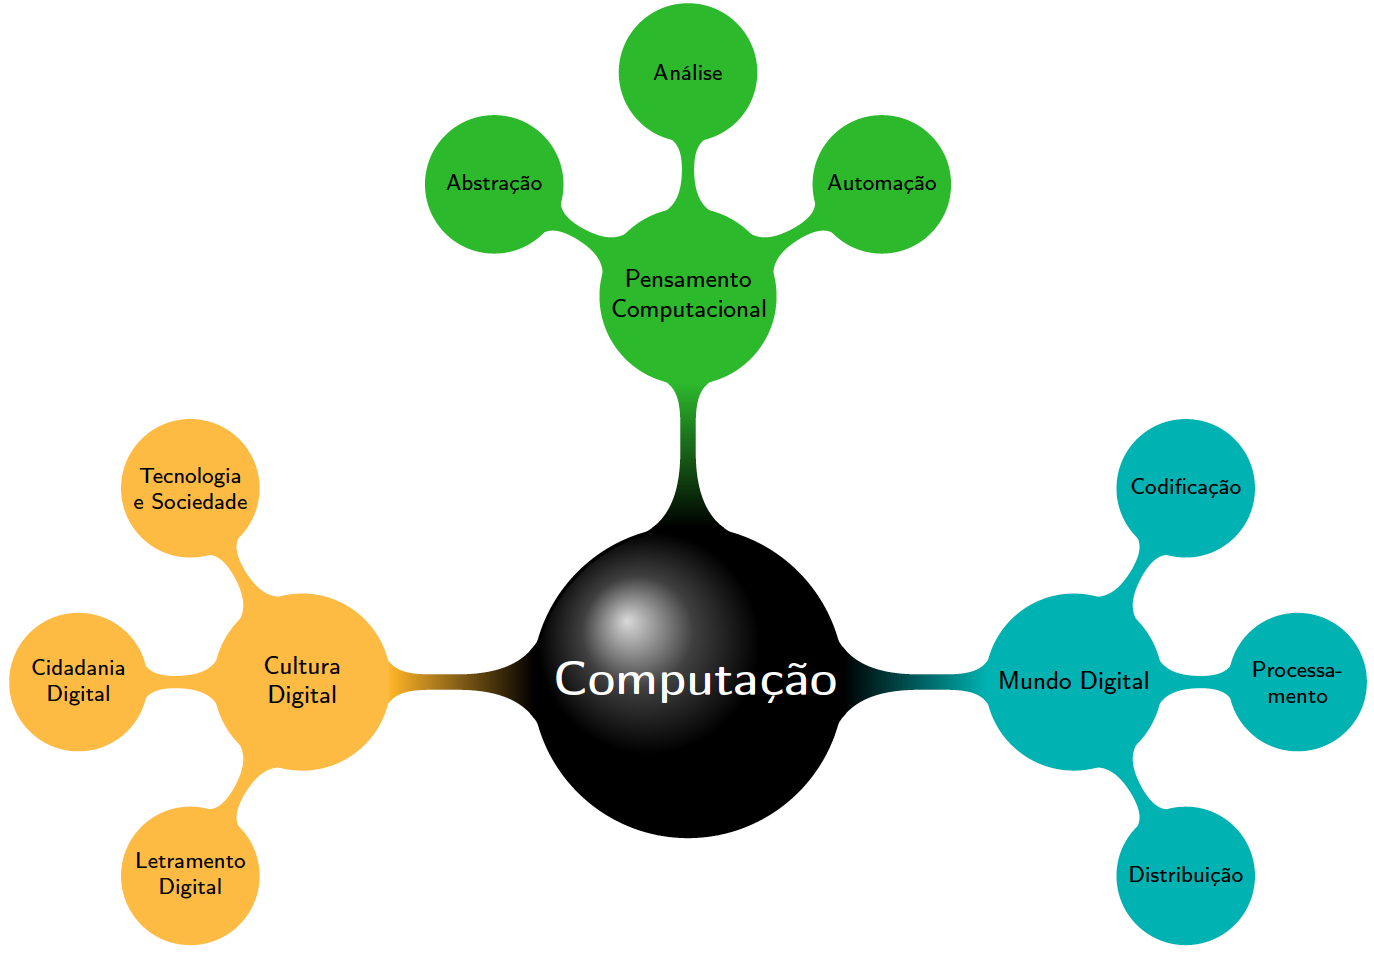
\includegraphics[scale=0.25]{eixos_computacao.png}
    \caption{Eixos da Computação \citep{ribeiro2019diretrizes}.}
    \label{figure:eixos_computacao}
\end{figure}

\section**{O uso de ferramentas no ensino de Computação}

É possível perceber que o ensino de Computação não se limita à aprendizagem de uma linguagem de programação. Ela é apenas uma ferramenta utilizada para aplicar estes conceitos de forma a chegar na solução de problemas, a partir do conhecimento de teoria da Computação e paradigmas de programação \citep{blatt2017mapeamento}. Assim, diferentes metodologias podem ser adotadas no ensino de programação para crianças e jovens e o uso de recursos didáticos apropriados, ferramentas ou aplicativos pedagógicos, é indispensável no aprendizado desses conceitos.

Há diversas maneiras de explorar a aprendizagem dos conceitos de Computação: jogos, programação visual, programação com blocos, kits de robótica, simulações, \textit{storytelling}, entre outras. Dentre as ferramentas utilizadas no ensino fundamental, nota-se uma preferência pelas linguagens visuais e plataformas focadas no ensino dos fundamentos (e não no desenvolvimento) \citep{gomes2017ensino}. A linguagem de programação em blocos é uma das mais citadas em estudos, apresentando diversas opções de ferramentas \citep{brezolin2021panorama,desouza2021ensino}. 

Deste modo, \textit{softwares} de apoio ao ensino de programação devem facilitar a compreensão das abstrações envolvidas nos conceitos de Computação, bem como, estimular o raciocínio lógico. Nesse sentido, o uso de simulações interativas facilita a visualização de conceitos abstratos, utilizando exemplos concretos para representá-los. 

Alguns trabalhos mostram a efetividade das simulações no ensino em outras áreas. Em particular, a plataforma de simulações interativas PhET (\textit{Physics Education Technology}) é um recurso bastante utilizado em várias disciplinas de ciências \citep{khatri2013over}. Criado em 2002 pelo ganhador do prêmio Nobel de Física em 2001, Carl Wieman, o projeto da Universidade de Colorado Boulder apresenta atualmente 170 simulações interativas distribuídas nas áreas de Física, Química, Matemática, Ciências da Terra e Biologia, destinadas tanto a alunos da educação básica como de ensino superior.

Entre 2012 e 2013, a plataforma realizou uma pesquisa com docentes que utilizavam a ferramenta, recebendo cerca de 2.000 respostas de escolas nos Estados Unidos \citep{price2018and}. O estudo mostrou três aspectos que contribuem para a escolha da ferramenta na sala de aula. Primeiro, devido a sua flexibilidade, as simulações são utilizadas de diversas maneiras e com diferentes objetivos de aprendizagem, como entender conceitos, processos científicos e aumentar a motivação dos estudantes. Além disso, os docentes preferem que os estudantes tenham controle da simulação. Por fim, algumas propriedades percebidas das simulações foram a visualização, manipulabilidade e a capacidade de realizar demonstrações que não poderiam ser feitas em sala.

No Brasil, diversos estudos mostram pontos positivos da utilização dessa ferramenta como forma de agregar ao ensino tradicional. Uma pesquisa bibliográfica de publicações de autores brasileiros entre os anos de 2010 e 2020, realizada por \citet{ramos2020ensino}, mostrou que a utilização do simulador PhET, junto a uma metodologia de ensino, potencializou o aprendizado dos estudantes, além de torná-los participantes ativos desse processo.

Outro trabalho, conduzido por \citet{cravo2021avaliaccao}, reforça essa conclusão. Eles avaliaram simulações de ciências e Biologia por meio de um protocolo de avaliação próprio e da realização de oficinas com futuros docentes, mostrando os desafios e potencialidade da ferramenta. Os autores concluíram que ela contribui positivamente no processo de ensino-aprendizagem, tornando-o mais didático e dinâmico,  e que a atuação de professores como mediadores do ensino pode ajudar a contornar possíveis deficiências na sua utilização. Ainda, os trabalhos de \citet{araujo2021uso,santos2020revisao} apresentam conclusões similares em relação ao uso de simulações no ensino de Física e Química, respectivamente.

Assim, esta é uma abordagem interessante a ser explorada também no ensino da Computação, pois da mesma forma que as ciências da natureza e das humanidades ajudam a explicar o mundo real, a Ciência da Computação ajuda a explicar o mundo digital \citep{ribeiro2019diretrizes}. Portanto, é natural que busquemos ferramentas análogas para o estudo dessas ciências e, até onde sabemos, não existem simulações de conceitos de lógica de programação iguais às encontradas no PhET.

\section**{Objetivos e contribuições}

Desse modo, este Trabalho de Formatura tem como objetivo a criação de um produto mínimo viável (MVP - \textit{Minimum Viable Product}) de uma ferramenta de simulações interativas para o ensino de conceitos de lógica de programação para crianças no ensino fundamental. Para isso, 
desenvolvemos uma versão da aplicação com um conjunto mínimo de requisitos, contendo uma simulação envolvendo alguns conceitos de lógica de programação. Além disso, queremos que os usuários tenham contato com a estrutura real do código de programação correspondente a cada conceito simulado. Assim, integramos à simulação uma visualização do pseudocódigo associado.

Também aplicamos o MVP em sala de aula para obter \textit{feedback} para um futuro desenvolvimento do sistema completo. Dessa forma, avaliamos a sua usabilidade com a ajuda de estudantes do ensino fundamental, por meio da aplicação de um questionário de usabilidade. Ademais, investigamos como representar os conceitos visualmente de forma que facilite a compreensão da lógica de programação por trás deles.

\pagestyle{mainmatter}
%!TeX root=../tese.tex
%("dica" para o editor de texto: este arquivo é parte de um documento maior)
% para saber mais: https://tex.stackexchange.com/q/78101

\chapter{Ferramentas pedagógicas para ensino de Computação}
\label{related_tools}

Como vimos no Capítulo de Introdução, o ensino de Computação não está ligado a uma linguagem de programação específica, mas sim à abstração dos conceitos de programação e ao conjunto de habilidades que envolvem o pensamento computacional. Desse modo, diferentes ferramentas e tecnologias são utilizadas no apoio às aulas de Computação nas escolas. A seguir, discutimos algumas das abordagens mais utilizadas no ensino de programação para crianças e adolescentes.

\section{Linguagem de programação visual em blocos}

A linguagem de programação visual em blocos se baseia na construção de algoritmos usando blocos lógicos de maneira simples e intuitiva. Essa abordagem é amplamente utilizada em diversas ferramentas. Podemos citar como principal exemplo o \textit{Scratch} \citep{scratch2024}, uma plataforma, que utiliza uma linguagem de programação visual baseada em blocos e permite criar estórias, jogos e animações. Criada inicialmente por um grupo do \textit{MIT Media Lab} (Laboratório de Mídia do Instituto de Tecnologia de Massachusetts) e desenvolvida atualmente pela \textit{Scratch Foundation}, ela é uma ferramenta gratuita e de código aberto, e está disponível em mais de 70 idiomas. Segundo seus desenvolvedores, ela promove o pensamento educacional, habilidades de resolução de problemas, criatividade, auto-expressão, colaboração e equidade.

A Figura \ref{figure:sctrach} apresenta a interface do \textit{Scratch}. O espaço à esquerda permite arrastar os blocos das diferentes categorias à área central da página, onde é montado o algoritmo. À direita, temos o resultado da execução do conjunto de blocos apresentado na forma de animações.

\begin{figure}[h!]
    \centering
    \setlength{\fboxrule}{0.1pt} % espessura da borda da figura
    \fbox{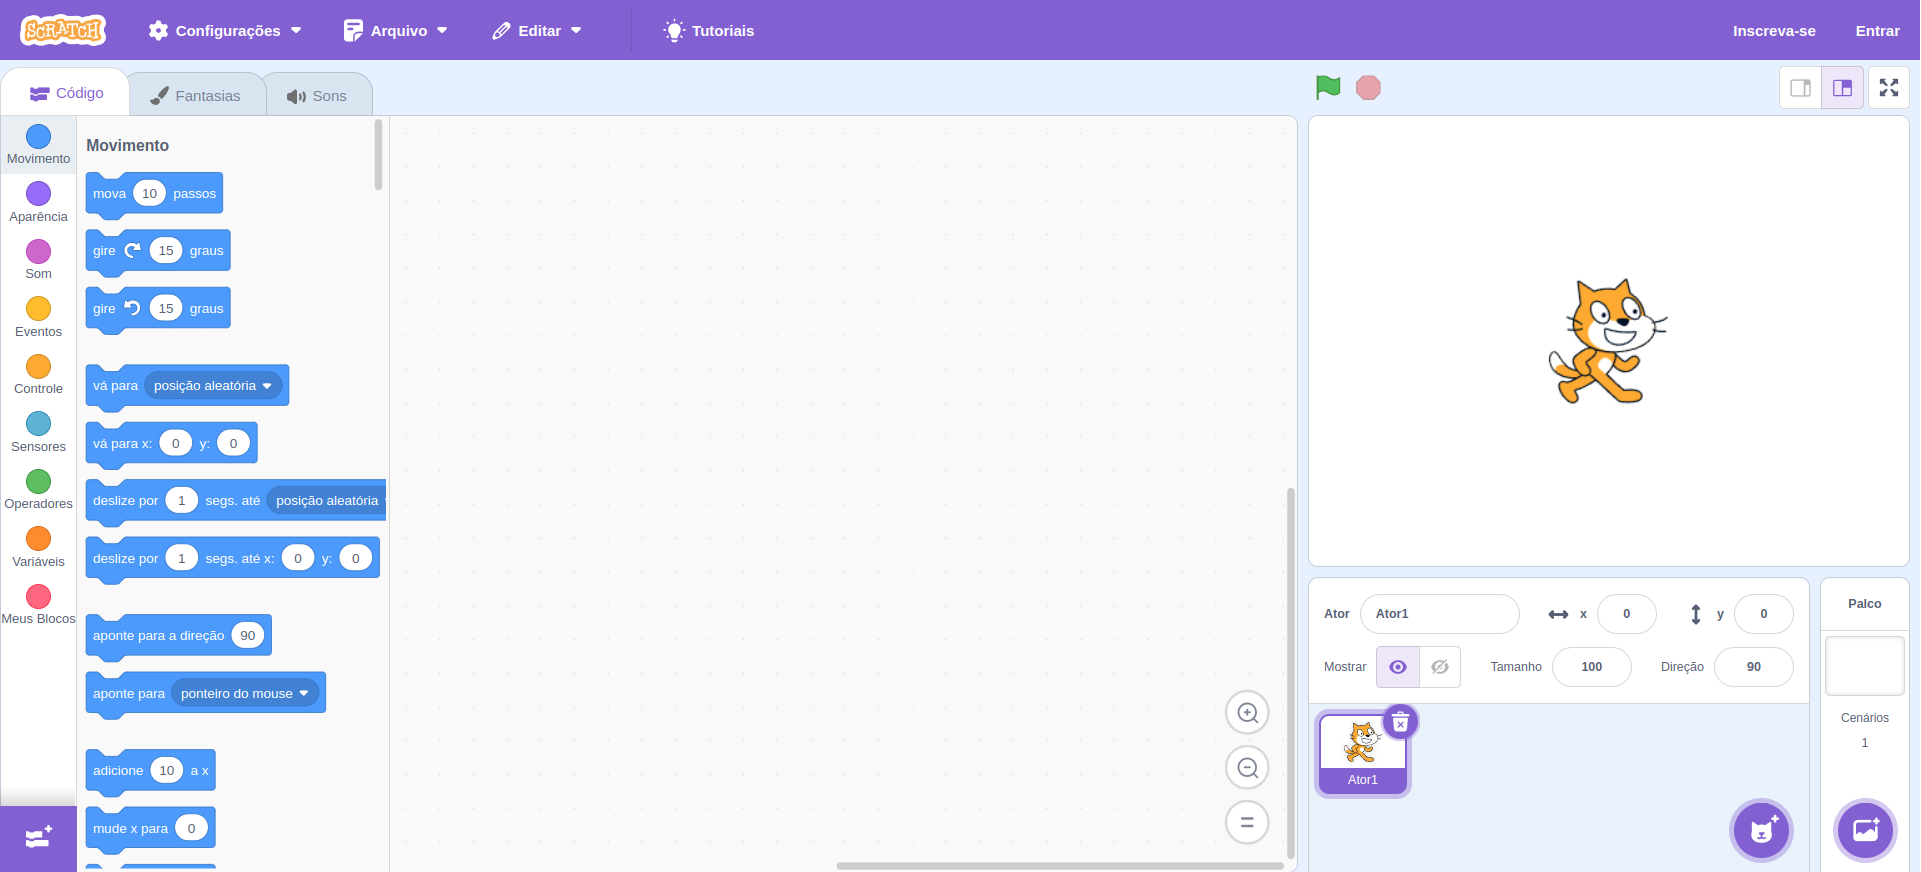
\includegraphics[scale=0.22]{scratch.png}}
    \caption{Interface do usuário da ferramenta \textit{Scratch} \citep{scratch2024}.}
    \label{figure:sctrach}
\end{figure}

Outra ferramenta baseada em blocos que merece destaque é o \textit{App Inventor} \citep{appinventor2024}, originalmente criado pelo Google e atualmente mantido pelo MIT. A plataforma permite a criação de aplicativos para os sistemas operacionais Android e iOS. Ela apresenta duas telas para a construção de um aplicativo: uma de design (Figura \ref{figure:app_inventor_design}), onde o visual do aplicativo pode ser montado, arrastando-se elementos visuais para a tela, como botões, texto de entrada, caixas de seleção, entres outros; e uma de blocos (Figura \ref{figure:app_inventor_logica}), onde é definida a lógica de interação com os elementos visuais adicionados como, por exemplo, qual efeito deve ser aplicado a um botão se ele for clicado.

\begin{figure}[t]
    \centering
    \setlength{\fboxrule}{0.1pt} % espessura da borda da figura
    \fbox{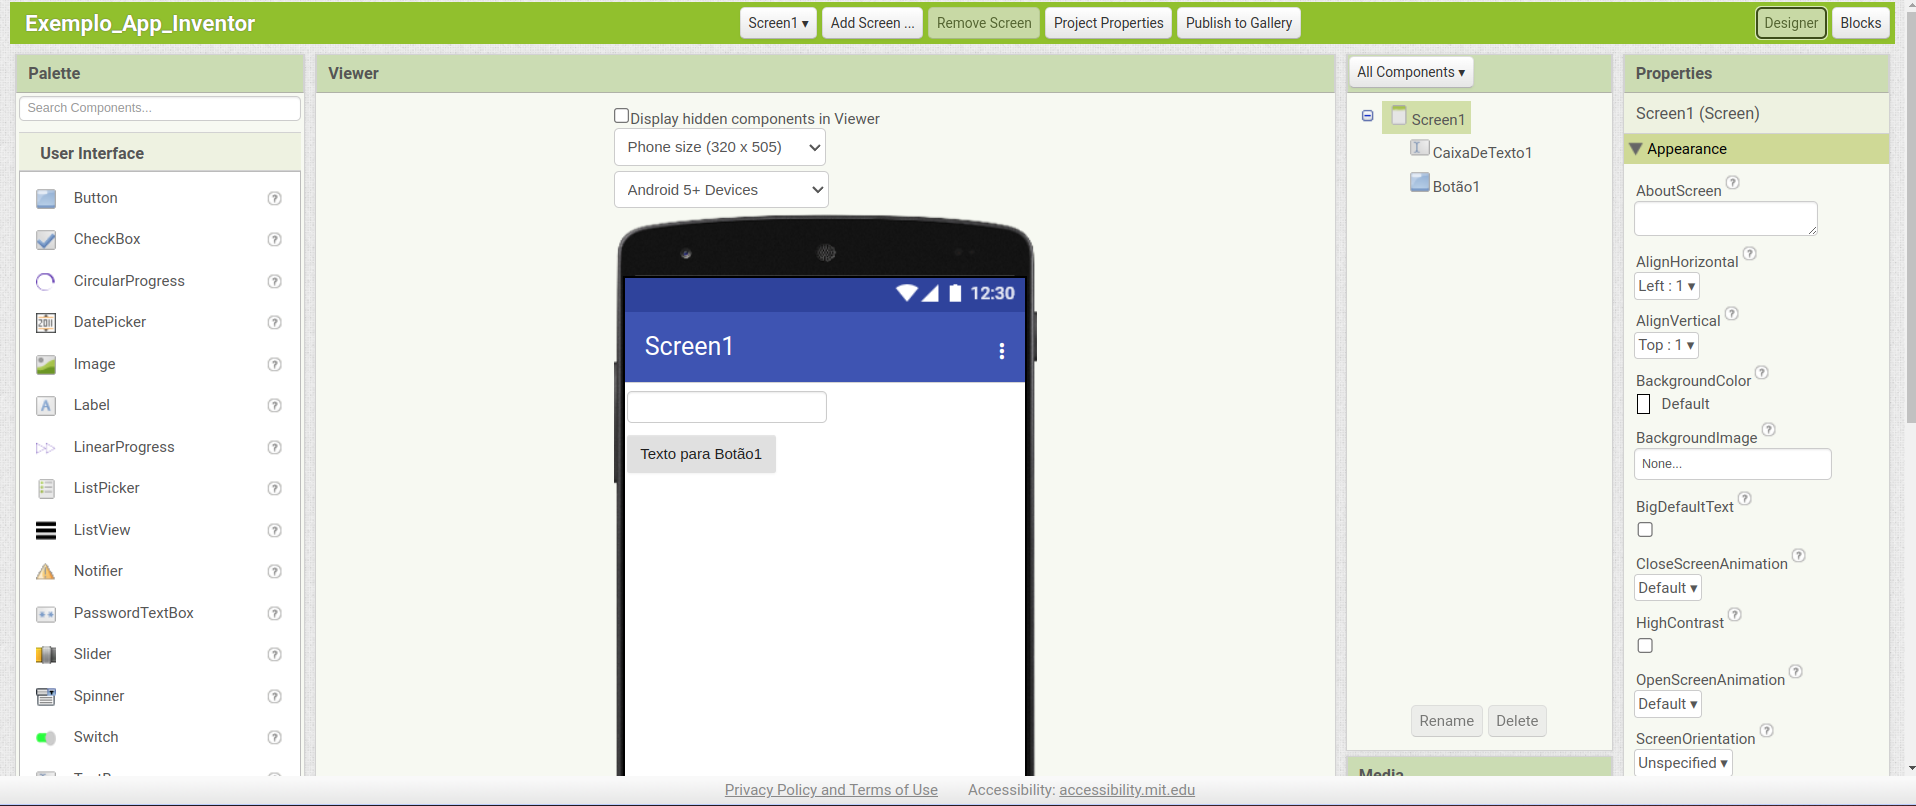
\includegraphics[scale=0.22]{figuras/app_inventor_design.png}}
    \caption{Interface do usuário da ferramenta \textit{App Inventor} para criar o design de um aplicativo \citep{appinventor2024}.}
    \label{figure:app_inventor_design}
\end{figure}

\begin{figure}[t]
    \centering
    \setlength{\fboxrule}{0.1pt} % espessura da borda da figura
    \fbox{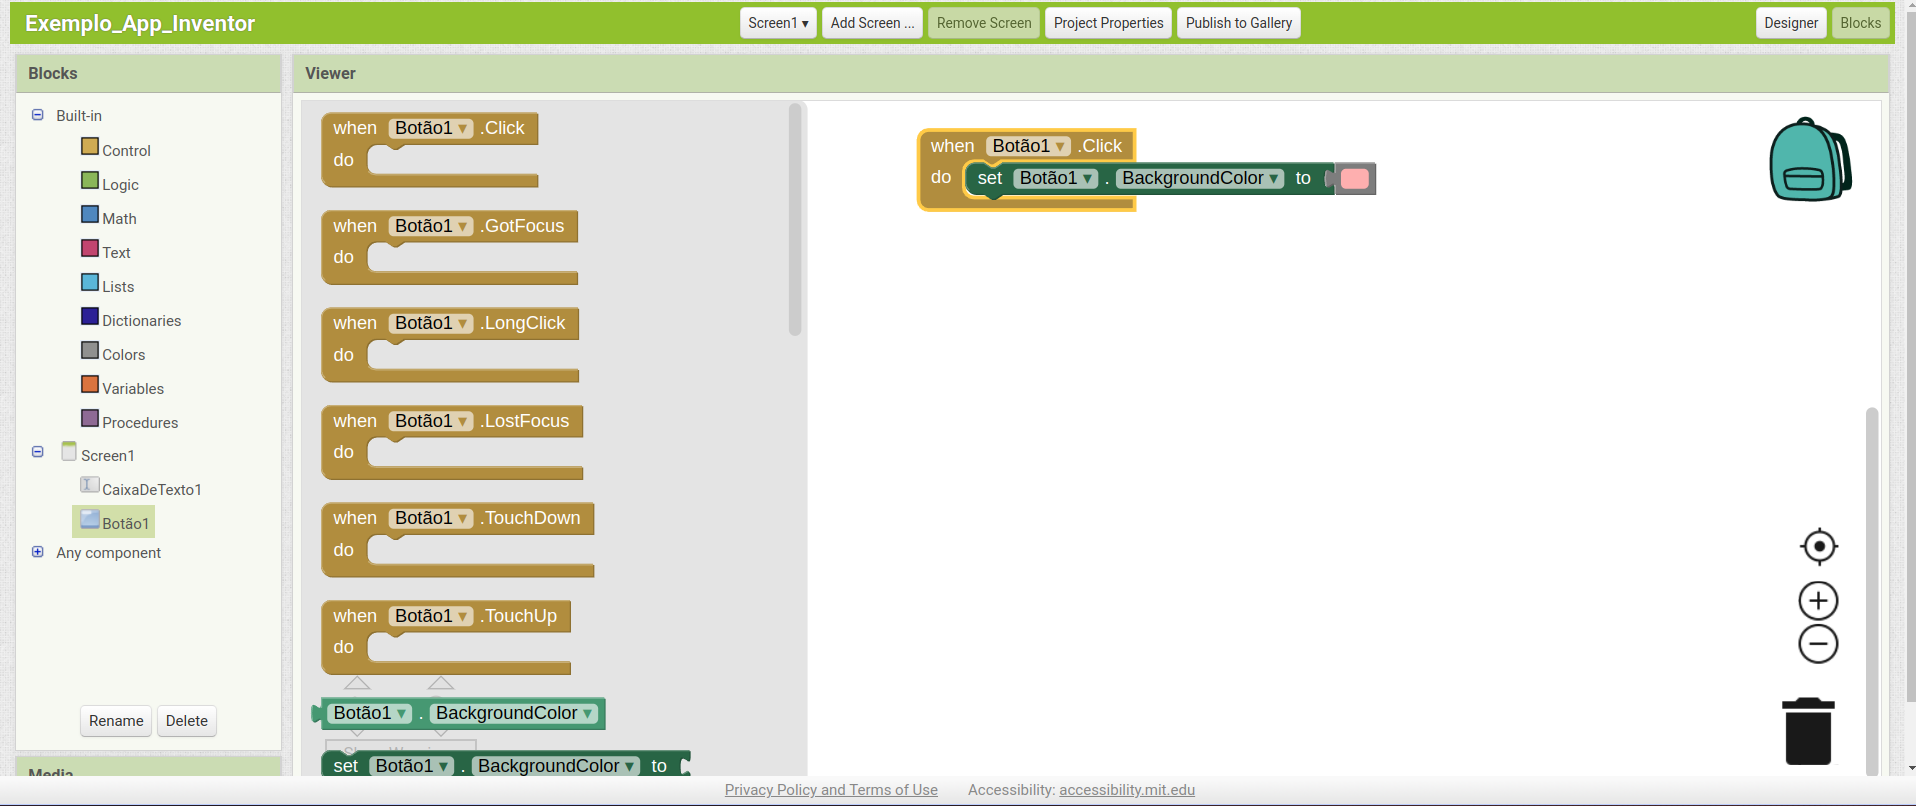
\includegraphics[scale=0.22]{figuras/app_inventor_logica.png}}
    \caption{Interface do usuário da ferramenta \textit{App Inventor} para criar a lógica de interação dos elementos do aplicativo \citep{appinventor2024}.}
    \label{figure:app_inventor_logica}
\end{figure}

Diversos estudos apontam esta abordagem, principalmente com o uso do \textit{Scratch}, como a mais utilizada no ensino de programação para crianças e adolescentes, apresentando resultados positivos \citep[e.g.][]{blatt2017mapeamento,bordini2016computaccao,khouri2020mapeamento,werlich2018pensamento}. Além disso, podemos observar que outras ferramentas, de jogos e robótica, por exemplo, também utilizam a linguagem visual em blocos em conjunto com sua metodologia principal. Alguns exemplos disso são: \textit{Blocky Games} \citep{blocklygames2024}, \textit{CodeCombat Junior} \citep{codecombat2024} e \textit{Lego Mindstorms} \citep{legomindstorms2024}.


\section{Jogos digitais}

A utilização de jogos digitais também pode estimular o pensamento computacional no ensino de programação. No geral, jogos fazem parte do cotidiano das crianças, além de aumentarem o engajamento e a motivação dos usuários. Um exemplo de jogo voltado para o ensino de programação é o \textit{CodeCombat} \citep{codecombat2024}, que permite que estudantes joguem e escrevam código utilizando uma linguagem baseada em texto com a sintaxe parecida com linguagens de programação. O jogo é gratuito e de código aberto, estando disponível em mais de 60 idiomas. Porém, a tradução para o português, muitas vezes, não é apresentada corretamente. A Figura \ref{figure:code_combate} apresenta a interface utilizada no \textit{CodeCombat}.

\begin{figure}[h!]
    \centering
    \setlength{\fboxrule}{0.1pt} % espessura da borda da figura
    \fbox{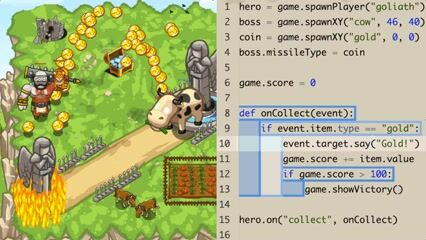
\includegraphics{figuras/code_combat.jpg}}
    \caption{Interface do usuário do jogo \textit{CodeCombat} \citep{codecombat2024}.}
    \label{figure:code_combate}
\end{figure}

Muitos desses jogos exploram comandos para orientar personagens, movendo-os para determinadas direções, e para realizar ações, utilizando de forma lúdica comandos com sintaxes muito similares a de funções das linguagens de programação.

\section{Kits de robótica}

Os kits de robótica combinam o uso de \textit{hardware} com o de software para o ensino de lógica de programação. A abordagem envolve a utilização de placas com microcontroladores e a montagem de circuitos ou robôs para realizarem determinadas tarefas como, por exemplo, um circuito ligado a lâmpadas de LED que poderão ser acesas ou um robô que irá andar alguns centímetros sobre o chão. O software, então, é utilizado para criar um programa que determina os comandos de execução dessas ações.

Um kit muito utilizado devido ao seu menor custo é o do Arduíno, que visa o controle de dispositivos, como LED e motores, ou a medição de variáveis, como temperatura e luminosidade. Ele requer conhecimentos em eletrônica por parte dos docentes e sua programação é feita através de um ambiente de desenvolvimento próprio baseado na linguagem de programação C \citep{klinczak2024estudo,demedeiros2019ensino}. Para facilitar a utilização deste tipo de ensino, algumas iniciativas criaram \textit{softwares} baseados na linguagem visual em blocos do \textit{Scratch} para escrever programas (Figura \ref{figure:arduino}).

\begin{figure}[h!]
    \centering
    \setlength{\fboxrule}{0.1pt} % espessura da borda da figura
    \fbox{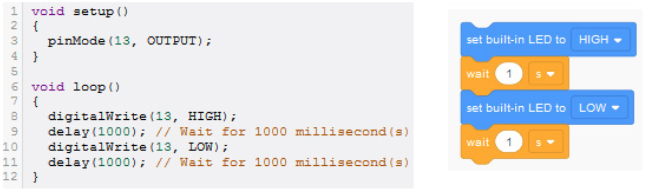
\includegraphics[scale=0.65]{figuras/arduino.png}}
    \caption{Exemplo da utilização da linguagem do \textit{Scratch} para programação do Arduíno \citep{demedeiros2019ensino}.}
    \label{figure:arduino}
\end{figure}

Outro exemplo com um custo mais elevado é o Kit educativo \textit{Lego Mindstorms}, o qual permite construir e programar um robô que pode andar, falar e pensar \citep{legomindstorms2024}. Sua montagem não requer conhecimentos de eletrônica, bastando apenas encaixar suas peças sem a necessidade de outras ferramentas (Figura \ref{figure:legomindstorms}). Também possui um ambiente próprio de programação visual, disponibilizado no site do fabricante.

\begin{figure}[h!]
    \centering
    \setlength{\fboxrule}{0.1pt} % espessura da borda da figura
    \fbox{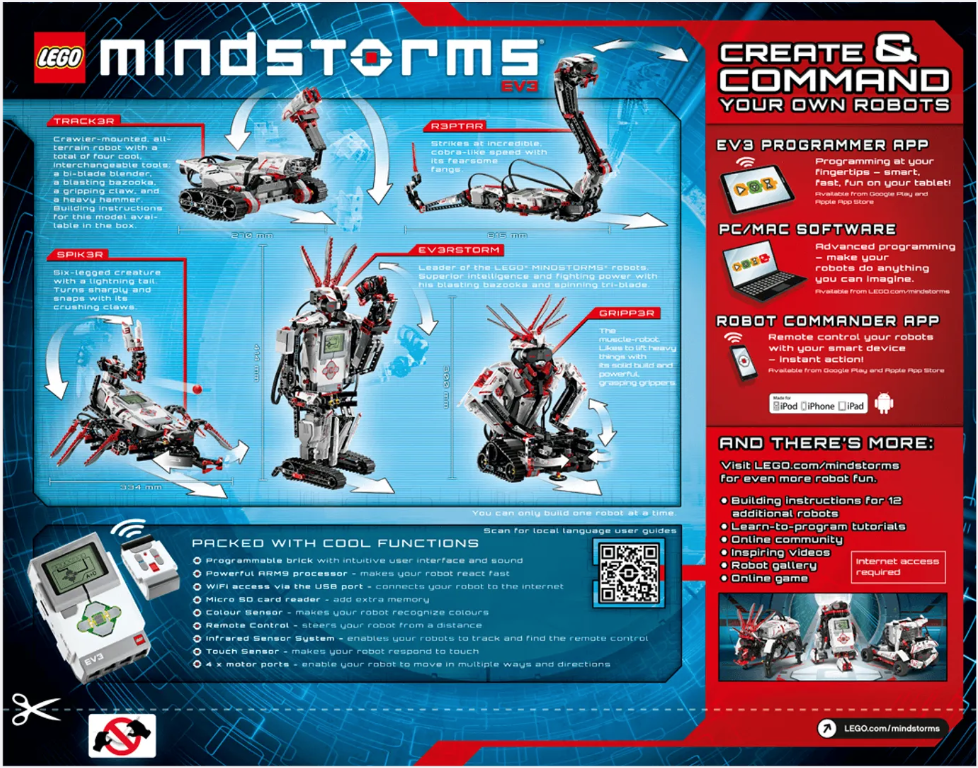
\includegraphics[scale=0.4]{figuras/lego_mindstorms.png}}
    \caption{Panorama o kit educativo \textit{Lego Mindstorms EV3} \citep{legomindstorms2024}.}
    \label{figure:legomindstorms}
\end{figure}

\section{Computação desplugada}

A Computação desplugada envolve atividades lúdicas que não necessitam do uso de computadores e podem abordar tópicos que ensinam conceitos de Computação, podendo ser realizadas por pessoas de quaisquer faixas etárias \citep{brackmann2017desenvolvimento}. Muitas vezes, as atividades envolvem ações de recortar, dobrar, colar, desenhar, pintar, resolver problemas, e os estudantes podem trabalhar em conjunto, promovendo habilidades de criatividade e colaboração. A Figura \ref{figure:desplugada} apresenta a descrição de um exemplo criado por \citet{brackmann2017desenvolvimento} em sua pesquisa sobre o desenvolvimento do pensamento computacional por meio de atividades desplugadas na educação básica.

\begin{figure}[h!]
    \centering
    \setlength{\fboxrule}{0.1pt} % espessura da borda da figura
    \fbox{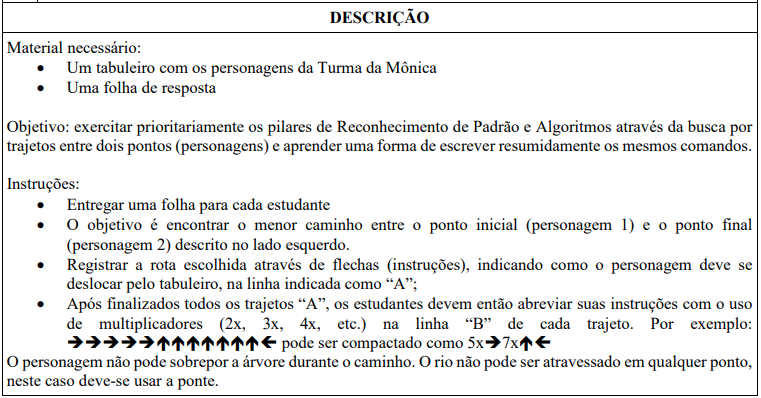
\includegraphics[scale=0.5]{figuras/desplugada.png}}
    \caption{Descrição de um exemplo de atividade desplugada \citep{brackmann2017desenvolvimento}.}
    \label{figure:desplugada}
\end{figure}

\section{Simulações interativas}

Simulações interativas utilizam elementos visuais do dia-a-dia para representar as abstrações envolvidas nos conceitos de diversas ciências, os quais não podemos ver ou manipular. Elas auxiliam no aprendizado desses tópicos, uma vez que os estudantes conseguem ver e manipular as interações \citep{price2018and}. Entretanto, ainda não existem muitas ferramentas que utilizem simulações interativas para o ensino de conceitos de lógica de programação. Em particular, não encontramos nenhuma ferramenta que se assemelhe a abordagem utilizada, de maneira bem-sucedida, pela plataforma PhET.

\citet{fernandes2012animacoes} criaram e avaliaram um objeto de aprendizagem na forma de animações e simulações no tema de variáveis de lógica de programação. O protótipo apresentava três partes: contextualização do conceito (sem interatividade), simulação de teste e fluxo de dados e uma atividade de fixação (Figura \ref{figure:oa}). Esse objeto de aprendizagem foi, então, avaliado por alunos e professores e os resultados obtidos demonstraram o potencial dessa abordagem. Porém, esse protótipo não foi encontrado disponível no link indicado no artigo.

\begin{figure}[h!]
    \centering
    \setlength{\fboxrule}{0.1pt} % espessura da borda da figura
    \fbox{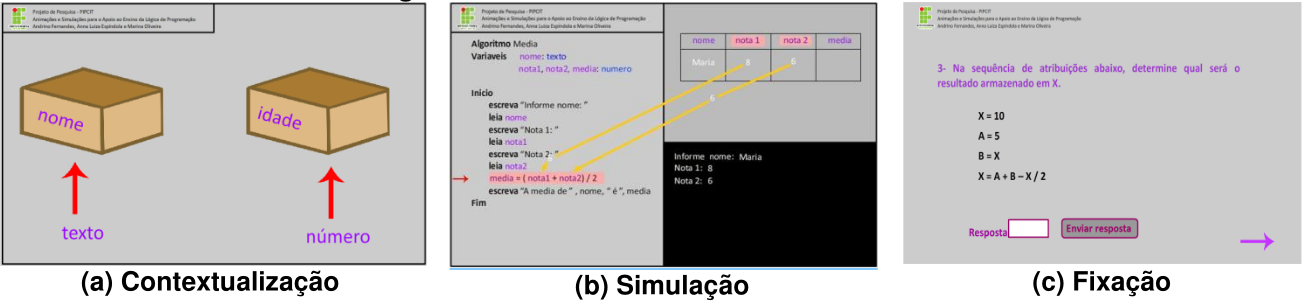
\includegraphics[scale=0.32]{figuras/objeto_aprendizagem.png}}
    \caption{Ilustração do objeto de aprendizagem de variáveis desenvolvido por \citet{fernandes2012animacoes}.}
    \label{figure:oa}
\end{figure}

Um outro exemplo encontrado, foi a ferramenta \textit{Drone Blocks} \citep{droneblocks2024}, um simulador de drones com programas projetados para o ensino de fundamentos de Ciência da Computação, entre outras finalidades não relacionadas a educação. A interface da simulação criada para o ensino (Figura \ref{figure:drone_blocks}) é muito similar a do \textit{Scratch}, a ferramenta utiliza a linguagem visual em blocos para construir instruções para o drone dentro de um cenário de sala de aula. Observamos como limitações dessa ferramenta o fato dela se restringir a simulações no contexto do drone na sala de aula e estar disponível apenas no idioma Inglês.

\begin{figure}[h!]
    \centering
    \setlength{\fboxrule}{0.1pt} % espessura da borda da figura
    \fbox{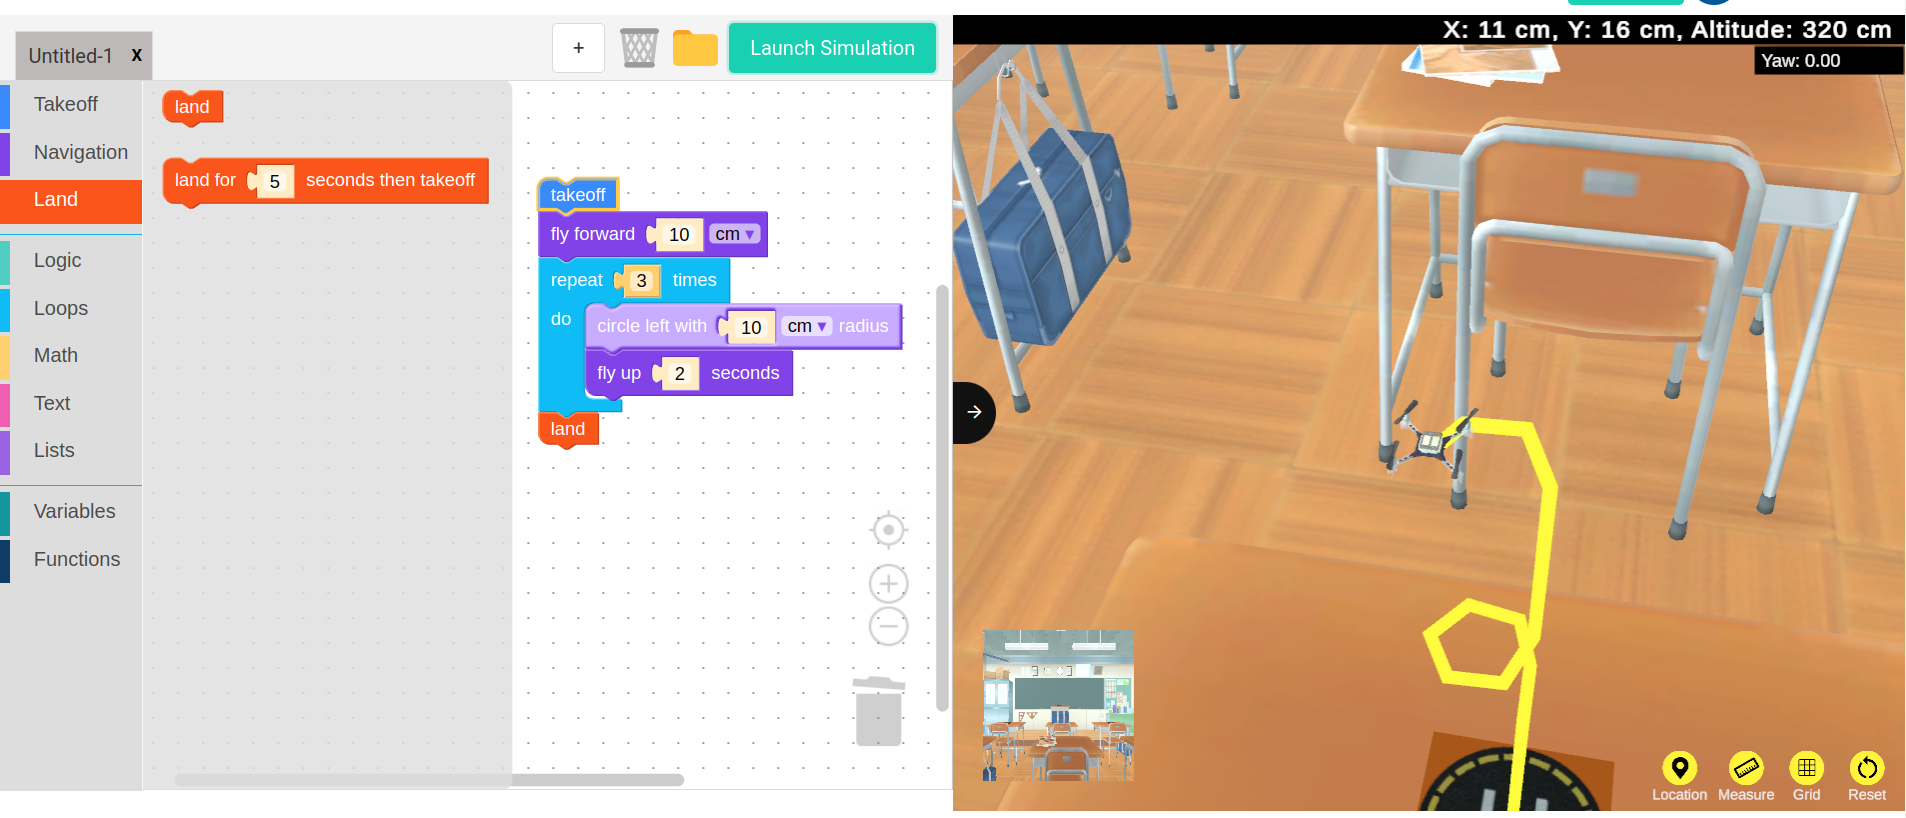
\includegraphics[scale=0.22]{figuras/drone_blocks.png}}
    \caption{Interface do usuário da simulação \textit{Drone Blocks} \citep{droneblocks2024}.}
    \label{figure:drone_blocks}
\end{figure}

Dessa maneira, o MVP proposto neste projeto tem um caráter inovador, uma vez que não foram encontradas, até o momento, outras ferramentas com propostas similares. Além disso, ele difere das demais abordagens apresentadas, pois na maioria delas o usuário constrói um código para visualizar a execução dele em forma de jogos, animações, histórias e aplicações. Já no protótipo proposto, há a interação com os elementos visuais da simulação e o pseudocódigo correspondente pode ser observado através dessas interações. Ainda, optamos por utilizar o pseudocódigo ao invés da linguagem de programação visual em blocos a fim de promover o contato com a estrutura real de um código fonte.
%!TeX root=../tese.tex
%("dica" para o editor de texto: este arquivo é parte de um documento maior)
% para saber mais: https://tex.stackexchange.com/q/78101

\chapter{Metodologia de pesquisa} 

Para criar e avaliar o MVP proposto, seguimos a metodologia de pesquisa de \textit{Design Science}, que de forma geral envolve a elaboração de artefatos para solucionar problemas em um contexto. Neste Capítulo, explicamos o que é a \textit{Design Science Research} e como ela foi conduzida neste projeto.

\section**{\textit{Design Science Research}}

A \textit{Design Science Research} (DSR) é uma metodologia de pesquisa utilizada na elaboração de artefatos com propósitos práticos, constituindo um processo de resolução de problemas de domínio, em que o resultado deve ser avaliado pelo seu valor e utilidade. Esse paradigma é aplicado em diferentes áreas de pesquisa, como Sistemas de Informação, Gerenciamento de Negócios, Engenharia de \textit{Software}, etc, podendo ser instanciado em variantes muito diferentes \citep{dresch2015design, runeson2020design}.

\citet{hevner2004design} definiram sete diretrizes para a realização de DSR na área de Sistemas de Informação, que têm como princípio a construção e aplicação de um artefato para adquirir conhecimento sobre um problema de design e sua solução. Assim, uma pesquisa em \textit{Design Science} requer a criação de um artefato com propósito para tecnologia da informação e com caráter inovador (diretriz 1), o qual deve considerar a solução de um problema de negócio relevante (diretriz 2). Além disso, o seu design deve ser avaliado rigorosamente considerando sua utilidade, qualidade e eficácia (diretriz 3). O artefato também deve ser inovador, proporcionando contribuições claras e verificáveis para pesquisa (diretriz 4), e sua construção e avaliação devem ser feitas de forma rigorosa (diretriz 5). O processo de design do artefato deve ser conduzido como um processo de pesquisa de uma solução efetiva para um problema (diretriz 6). Por fim, os resultados da pesquisa em \textit{Design Science} devem ser comunicados de forma eficaz (diretriz 7).

%%%%%%%%%%%%%%%%%%%%%%%%%%%%%%%%%%%%%%%%%%%%%%%%%%%%%%%%%%%%%%%%%%%%%%%%%%%%%%%%
%%% Diretrizes Hevner (2004)
% \begin{enumerate}
%     \item \textbf{Design como um artefato:} criação de um artefato com propósito para TI e com caráter inovador
%     \item \textbf{Relevância do problema:} o artefato deve considerar a solução de um problema de negócios relevante
%     \item \textbf{Avaliação do design:} o design do artefato deve ser avaliado rigorosamente considerando sua utilidade, qualidade e eficácia
%     \item \textbf{Contribuições de pesquisa:} o artefato deve ser inovador, proporcionando contribuições claras e verificáveis para pesquisa
%     \item \textbf{Rigor de pesquisa:} a construção e avaliação do artefato projetado devem ser feitas de forma rigorosa
%     \item \textbf{Design como um processo de pesquisa:} o processo de design do artefato é um processo de pesquisa de uma solução efetiva para um problema
%     \item \textbf{Comunicação da pesquisa:} os resultados da pesquisa em Design Science devem ser comunicados de forma efetiva
% \end{enumerate}
%%%%%%%%%%%%%%%%%%%%%%%%%%%%%%%%%%%%%%%%%%%%%%%%%%%%%%%%%%%%%%%%%%%%%%%%%%%%%%%%

\citet{wieringa2014design} estendeu a definição de \textit{Design Science}, apresentando diretrizes para realizar pesquisas em Sistemas de Informação e Engenharia de \textit{Software}. Para o autor, a interação entre o artefato e o contexto do problema contribui para chegar à solução do problema. Dessa forma, um projeto de DS itera sobre as atividades de design e investigação. A atividade de design é decomposta em três tarefas, designadas como ciclo de design. Esse ciclo está inserido em um outro, de engenharia, no qual temos o resultado do ciclo de design sendo introduzido no contexto real e avaliado. As etapas de cada um dos ciclos estão descritas a seguir:

\noindent \textbf{Ciclo de engenharia:}

\begin{itemize}
    \item \textbf{Ciclo de design:}
    \begin{itemize}
        \item \textbf{Investigação do problema:} qual problema deve ser investigado e por quê?
        \item \textbf{Design do tratamento (\textit{Treatment design}):} projeto de um ou mais artefatos para tratar o problema.
        \item \textbf{Validação do tratamento (\textit{Treatment validation}):} análise para validar se esse projeto contribui para o tratamento do problema, caso seja implementado.
    \end{itemize}
    \item \textbf{Implementação do tratamento (\textit{Treatment implementation}):} tratamento do problema com um dos artefatos projetados.
    \item \textbf{Avaliação da implementação (\textit{Implementation evaluation}):} avaliação do sucesso do tratamento. Ao final dessa etapa, podemos ter uma nova iteração no ciclo de engenharia.
\end{itemize}

\noindent O autor também destaca que projetos de pesquisa em \textit{Design Science} estão relacionados apenas às três etapas do ciclo de \textit{design}.

\citet{runeson2020design} define etapas similares para o ciclo de engenharia, envolvendo a conceitualização do problema, o projeto da solução e a validação empírica. Os autores explicam que a \textit{Design Science} abrange duas dimensões principais: problema-solução e teoria-prática. Eles descrevem as atividades de pesquisa que são realizadas de forma iterativa através das duas dimensões, são elas:

\begin{itemize}
    \item \textbf{Conceitualização do problema:} descrição do problema.
    \item \textbf{\textit{Design} da solução:} mapeamento do problema para uma solução geral.
    \item \textbf{Abstração:} identificação de decisões de \textit{design} importantes para uma solução válida dentro de um escopo definido.
    \item \textbf{Instanciação:} implementação do artefato em contexto.
    \item \textbf{Validação empírica:} avaliação de como a solução implementada abordou o problema.
\end{itemize}

Ademais, projetos de pesquisa em \textit{Design Science} devem considerar dois fatores importantes: a relevância da pesquisa para entidades na resolução de problemas reais e o rigor para que a pesquisa seja considerada válida e confiável, contribuindo para uma determinada área. Dessa forma, a DSR é importante tanto para a produção de conhecimento científico como para a resolução de problemas reais \citep{dresch2015design, runeson2020design}.

Portanto, a \textit{Design Science} aborda problemas gerais através do estudo de instâncias específicas de problemas no contexto de pesquisa. Para realizar este Trabalho de Formatura, seguimos a metodologia de \textit{Design Science Research} em Engenharia de Software proposta por \citet{wieringa2014design}, englobando o ciclo de \textit{design} e de engenharia. Nas seções a seguir, descrevemos as etapas de cada ciclo referentes a este trabalho.

\section{Ciclo de \textit{design}}

\subsection{Investigação do problema}
% Qual problema deve ser investigado e por quê?

O problema investigado neste estudo foi o de uso de simulações interativas no ensino de conceitos de lógica de programação para crianças. Como apresentado no Capítulo~\ref{related_tools}, diferentes metodologias são adotadas para isso, utilizando recursos didáticos variados, sendo as linguagens visuais as mais utilizadas. Dessa maneira, investigamos o uso de simulações interativas para o ensino de Computação, uma vez que elas podem facilitar a visualização de ideias abstratas envolvidas nos conceitos de programação, utilizando exemplos concretos para representá-las. Ademais, essa metodologia se mostrou eficaz em outras ciências, com o uso da ferramenta PhET. Portanto, queremos expandi-la e testá-la em outros ambientes de aprendizado, como na área de Ciência da Computação.

%%%%%%%%%%%%%%%%%%%%%%%%%%%%%%%%%%%%%%%%%%%%%%%%%%%%%%%%%%%%%%%%%%%%%%%%%%%%%%%%
% Problema?
% - representações visuais dos conceitos de lógica de programação para o ensino de Computação para crianças
% - nova abordagem para ensino dos conceitos de lógica de programação para crianças
%
% Etapas
% - estudo sobre o ensino de Computação para crianças
% - busca extensiva de ferramentas de apoio pedagógico existentes
%%%%%%%%%%%%%%%%%%%%%%%%%%%%%%%%%%%%%%%%%%%%%%%%%%%%%%%%%%%%%%%%%%%%%%%%%%%%%%%%

Para investigar o problema, primeiramente, realizamos uma pesquisa sobre o estado atual do ensino de Computação para crianças em escolas no Brasil e no mundo. Em seguida, fizemos uma busca extensiva dos diversos tipos de ferramentas de apoio pedagógico existentes e similares a proposta neste trabalho, procurando entender as principais diferenças entre elas. Grande parte dessa pesquisa foi realizada durante o desenvolvimento do projeto de Iniciação Científica (IC) intitulado \enquote{Uma Ferramenta de Simulações Interativas para Ensino de Computação para Crianças}, realizado entre outubro de 2022 e outubro de 2023. O resumo dos principais resultados dessa investigação se encontra nos Capítulos \ref{introduction} e \ref{related_tools} desta monografia.

\subsection{Projeto do artefato} \label{design}
% projeto de um ou mais artefatos para tratar o problema.

O artefato projetado como tratamento do problema é um MVP de uma ferramenta de simulações interativas de conceitos de lógica de programação destinada a crianças do ensino fundamental. Um MVP (\textit{Minimum Viable Product}) ou produto mínimo viável é um produto com funcionalidades suficientes para ser utilizado por usuários iniciais que possam fornecer \textit{feedback} com o intuito de validar uma ideia. 

No ensino da Computação, alguns conceitos introdutórios são fundamentais para o aprendizado da lógica de programação, tais como variáveis, entrada e saída de dados, operadores lógicos e aritméticos, condicionais, laços de repetição, funções, vetores, matrizes, entre outros. Desse modo, para testar a viabilidade do protótipo proposto, seu projeto deve compreender um conjunto mínimo desses conceitos, a fim de verificar o entendimento deles pelos usuários. 

Assim, para projetar os artefatos ou protótipos do MVP, primeiramente, definimos alguns requisitos mínimos, listados a seguir:

\begin{itemize}
    \item O MVP deve apresentar uma tela com uma área de trabalho e uma opção de ajuda com uma documentação explicativa de uso;
    \item A área de trabalho deve apresentar um espaço fixo para a simulação e outro para o pseudocódigo correspondente;
    \item A simulação deve envolver os seguintes conceitos de lógica de programação: variáveis, entrada, saída, operadores (aritméticos, lógicos e de comparação), condicionais e laços de repetição;
    \item A simulação deve apresentar um número limitado de interações possíveis com o usuário;
    \item A simulação deve encorajar os usuários a explorá-la livremente, com controles intuitivos e uma interface que possibilite boa usabilidade;
    \item O pseudocódigo deve ser gerado automaticamente conforme as interações com a simulação vão ocorrendo.
\end{itemize}

Além disso, também definimos e descrevemos os conceitos de lógica de programação que foram simulados e a sintaxe do pseudocódigo gerado. A partir dos protótipos iniciais, estudamos ideias similares e validamos os artefatos projetados para analisar alterações necessárias e as melhores opções de implementação. O Capítulo \ref{prototypes} apresenta em detalhes o desenvolvimento dos protótipos propostos.

\subsection{Validação do artefato} \label{validation}
% análise para validar se esse projeto contribui para o tratamento do problema, caso seja implementado
A validação dos artefatos foi realizada com base nas opiniões de profissionais de ensino de Computação e matemática. Foram consultados: a professora Dra. Kelly Braghetto do Departamento de Ciência da Computação do IME, minha orientadora no trabalho de formatura, que também coordena o projeto CodificADAs USP, oferecendo cursos introdutórios de programação voltados para meninas do ensino médio; a estudante Victoria Nóvoa, do curso de Licenciatura em Educomunicação da USP, instrutora de tecnologia educacional de crianças no Colégio Santa Cruz; e o professor Henri Silva da Escola de Aplicação da Faculdade de Educação da USP, que leciona matemática para alunos do 8° ano do Ensino Fundamental II.

Em conversas com os avaliadores, foi possível obter \textit{feedbacks} para verificar a usabilidade e utilidade do MVP a partir dos protótipos projetados, possibilitando o refinamento deles e a escolha de um artefato para implementação, além da definição do público alvo específico para testar a aplicação. No Capítulo \ref{prototypes}, descrevemos o processo de validação e as alterações realizadas. 

\section{Ciclo de engenharia}

Após a execução das etapas anteriores, completando uma iteração no ciclo de \textit{design}, realizamos os demais passos do ciclo de engenharia, descritos a seguir.

\subsection{Implementação da simulação}
% tratamento do problema com um dos artefatos projetados
O MVP da simulação foi desenvolvido utilizando o \textit{framework} de código aberto Vue.js\footnote{\url{https://vuejs.org/}}, que é muito utilizado para criar aplicações de página única (\textit{single-page applications}), com a intenção de agilizar o desenvolvimento, permitindo a utilização de soluções existentes e reduzindo a necessidade de escrever códigos do zero. O projeto criado com o \textit{framework} foi inicializado para ser utilizado com a linguagem de programação Typescript. Em conjunto com o Vue.js, utilizamos o Vuetify\footnote{\url{https://vuetifyjs.com/en/}}, um \textit{framework} de componentes de UI de código aberto, que contém diversos \textit{layouts} prontos e componentes dinâmicos.

O código desenvolvido ao longo do projeto, com a implementação do artefato, está disponível no seguinte repositório: \url{https://github.com/mariliatd/logic-sims-mvp}, sob a licença MPL-2.0 (\textit{Mozilla Public License Version 2.0}). Para desenvolver o MVP, utilizamos a organização em componentes que o \textit{framework} Vue possibilita. Dessa maneira, foi possível definir cada conceito de lógica de programação como um componente isolado a ser reutilizado dentro de um \textit{template} de simulação, conforme necessário. Também separamos os componentes referentes aos elementos visuais da simulação do pseudocódigo, criando maior modularidade no código.

Assim, com o artefato implementado, criamos uma página para disponibilizar o MVP, através da ferramenta de versionamento de códigos GitHub, para a aplicação e avaliação da ferramenta em sala de aula.

\subsection{Avaliação da simulação}
% avaliação do sucesso do tratamento
A avaliação do MPV da ferramenta de simulação foi realizada utilizando um formulário de usabilidade e uma atividade para verificação do aprendizado dos conceitos de lógica de programação. Primeiramente, por meio do questionário de usabilidade, métrica comum na avaliação de um protótipo ou sistema, o MVP foi analisado considerando a facilidade de uso, de aprendizado e satisfação. Em particular, utilizamos o questionário SUS (\textit{System Usability Scale}), aplicado aos usuários finais.

Apesar de não haver medidas absolutas de usabilidade, é possível utilizar escalas gerais para comparar usabilidade em determinados contextos. O SUS representa uma escala de usabilidade com 10 itens que pode ser utilizada para avaliar sistemas \citep{brooke1996sus}. Ele é baseado na escala Likert, a qual contém afirmações e os avaliadores indicam o grau de concordância ou discordância com cada uma, que varia de 1 a 5. Recomenda-se que as respostas para cada item sejam registradas de imediato, sem que os respondentes levem muito tempo pensando nelas.

Para obter o \textit{score} de usabilidade do sistema a partir do questionário SUS, primeiramente, a contribuição de cada item é normalizada para uma escala de 0 a 4. Em seguida, a soma das pontuações dos itens é multiplicada por 2.5, obtendo um \textit{score} em uma escala de 0 a 100. Entretanto, os autores não revelaram como analisar esta pontuação.

\citet{bangor2008empirical, bangor2009determining} realizaram um estudo onde avaliaram a usabilidade de diversos produtos e serviços utilizando o questionário SUS. Eles analisaram a média de pontuação do SUS em 273 estudos com cerca de 3.500 pesquisas individuais. Os autores realizaram uma interpretação dessa pontuação, comparando os quartis dos \textit{scores}. Além disso, eles adicionaram uma afirmação ao questionário para avaliar a usabilidade do sistema através de uma escala de classificação de adjetivos, obtendo uma correlação entre eles e a média das pontuações. As médias que correspondem a cada adjetivo são as seguintes:

\begin{enumerate}
    \item pior imaginável (\textit{worst imaginable}): 12.5
    \item horrível (\textit{awful}) : 20.3
    \item ruim (\textit{poor}): 35.7
    \item ok (\textit{ok}): 50.9
    \item bom (\textit{good}): 71.4
    \item excelente (\textit{excellent}): 85.5
    \item melhor imaginável (\textit{best imaginable}): 90.9
\end{enumerate}

Os autores ainda expressaram preocupações com o uso do adjetivo \enquote{ok}, uma vez que ele sugere uma experiência aceitável com o sistema, enquanto a média de pontuações na faixa dele sugere deficiências. Eles acreditam que o termo \enquote{razoável} (\textit{fair}) seria melhor indicativo da usabilidade percebida pelos usuários.

Ademais, o SUS é considerado um questionário robusto e confiável, tendo sido utilizado em diversos projetos de pesquisa e avaliações na indústria \citep{brooke1996sus}. Embora não tenha sido projetado considerando necessidades específicas de compreensão por crianças, o questionário tem sido utilizado em vários estudos de testes e avaliações de ferramentas com crianças de diversas faixas etárias com sucesso \citep[i.e.][]{wronska2015ipad, dexheimer2017usability, sanchez2020usability, tasfia2023evaluating}. 

\citet{putnam2020adaptation} realizaram uma adaptação e teste do SUS com crianças na faixa etária de 7 a 11 anos. Os autores adaptaram o questionário, com o auxílio de professores da educação básica, em um contexto de aplicativos móveis de jogos focados no ensino de programação e pensamento computacional. As afirmações foram ainda modificadas pensando na separação de dois grupos de faixa etária, entre 7 e 8 anos e entre 9 e 11 anos. A Tabela \ref{table:sus} mostra os enunciados do SUS original e as adaptações propostas para os dois grupos mencionados, em inglês.  
Além das simplificações das afirmações, os autores também utilizaram uma representação visual da escala de Likert (Figura \ref{figure:likert}), sugerida pelos docentes participantes do experimento.
Os resultados obtidos nos experimentos mostraram que o questionário modificado juntamente com a escala visual foi compreendido pelas crianças participantes, necessitando apenas de clarificações mínimas. Eles ainda sugeriram alterações nas afirmações 6, 8 e 10 para melhorar a compreensão e a confiabilidade delas.


\begin{table}[h!]
\centering
\resizebox{\textwidth}{!}{%
\begin{tabular}{|c|c|c|c|}
\hline
\textbf{Afirmativa} & \textbf{SUS original}                                                                                                                 & \textbf{SUS adaptado: Grupo 9-11 anos}                                                                                                   & \textbf{SUS adaptado: Grupo 7-8 anos}                          \\ \hline
\textbf{1}           & \begin{tabular}[c]{@{}c@{}}I think that I would like to use this\\ system frequently.\end{tabular}                                    & \begin{tabular}[c]{@{}c@{}}If I had this {[}app{]} on my iPad, \\ I think that I would like to play it a lot.\end{tabular} & I would like to play {[}app{]} a lot more.       \\ \hline
\textbf{2}           & I found the system unnecessary complex.                                                                                               & \begin{tabular}[c]{@{}c@{}}I was confused many times \\ when I was playing {[}app{]}.\end{tabular}                         & {[}app{]} was hard to play.                      \\ \hline
\textbf{3}           & I thought the system was easy to use.                                                                                                 & I thought {[}app{]} was easy to use.                                                                                       & I thought {[}app{]} was easy to use.             \\ \hline
\textbf{4}           & \begin{tabular}[c]{@{}c@{}}I think that I would need the support of a\\  technical person to be able to use this system.\end{tabular} & \begin{tabular}[c]{@{}c@{}}I would need help from an\\  adult to continue to play {[}app{]}.\end{tabular}                  & I would need help to play {[}app{]} more.        \\ \hline
\textbf{5}           & \begin{tabular}[c]{@{}c@{}}I found the various functions in this\\ system were well integrated.\end{tabular}                          & \begin{tabular}[c]{@{}c@{}}I always felt like I knew what to do\\  next when I played {[}app{]}.\end{tabular}              & I knew what to do next when I played {[}app{]}.  \\ \hline
\textbf{6}           & \begin{tabular}[c]{@{}c@{}}I thought there was too much\\ inconsistency in the system.\end{tabular}                                   & \begin{tabular}[c]{@{}c@{}}Some of the things I had to do when\\  playing {[}app{]} did not make sense.\end{tabular}       & Some things in {[}app{]} made no sense.          \\ \hline
\textbf{7}           & \begin{tabular}[c]{@{}c@{}}I would imagine that most people would\\ learn to use this system very quickly.\end{tabular}               & \begin{tabular}[c]{@{}c@{}}I think most of my friends could\\  learn to play {[}app{]} very quickly.\end{tabular}          & {[}app{]} would be easy for my friends to learn. \\ \hline
\textbf{8}           & I felt the system was cumbersome to use.                                                                                              & \begin{tabular}[c]{@{}c@{}}Some of the things I had to do \\ to play {[}app{]} were kind of weird.\end{tabular}            & To play {[}app{]} I had to do some weird things. \\ \hline
\textbf{9}           & I felt very confident using the system.                                                                                               & I was confident when I was playing {[}app{]}.                                                                              & I was proud of how I played {[}app{]}.           \\ \hline
\textbf{10}          & \begin{tabular}[c]{@{}c@{}}I needed to learn a lot of things before\\ I could get going with this system.\end{tabular}                & \begin{tabular}[c]{@{}c@{}}I had to learn a lot of things \\ before playing {[}app{]} well.\end{tabular}                   & There was a lot to learn to play {[}app{]}.      \\ \hline
\end{tabular}%
}
\caption{Afirmativas em inglês do questionário de avaliação de usabilidade de sistemas SUS e adaptações propostas por \citet{putnam2020adaptation} para crianças entre 7 e 11 anos, dividida em dois grupos.}
\label{table:sus}
\end{table} 

\begin{figure}[h!]
    \centering
    \setlength{\fboxrule}{0.1pt} % espessura da borda da figura
    \fbox{\includegraphics[scale=0.5]{escalaLikertVisual.png}}
    \caption{Representação visual da escala de Likert \citep{putnam2020adaptation}.}
    \label{figure:likert}
\end{figure}


Dessa forma, utilizamos uma adaptação do questionário SUS para obter o \textit{feedback} dos estudantes sobre o MVP para avaliá-lo em relação a sua usabilidade.  
Ademais, através da atividade de aprendizado dos conceitos de programação, analisamos o potencial do ensino de Computação utilizando simulações interativas. No Capítulo \ref{evaluation}, descrevemos a atividade realizada em sala de aula com a aplicação dos dois formulários para avaliação do artefato implementado.

%!TeX root=../tese.tex
%("dica" para o editor de texto: este arquivo é parte de um documento maior)
% para saber mais: https://tex.stackexchange.com/q/78101

\chapter{Criação e validação dos protótipos da simulação}
\label{prototypes}

A partir dos requisitos listados no Capítulo \ref{design}, criamos dois protótipos iniciais de simulações desenvolvidos no Figma\footnote{\url{https://www.figma.com/}}, uma plataforma \textit{web} colaborativa para projetar interfaces. As Figuras~\ref{figure:brinquedos1} e~\ref{figure:festa1} mostram esses protótipos.

\begin{figure}[h!]
    \centering
    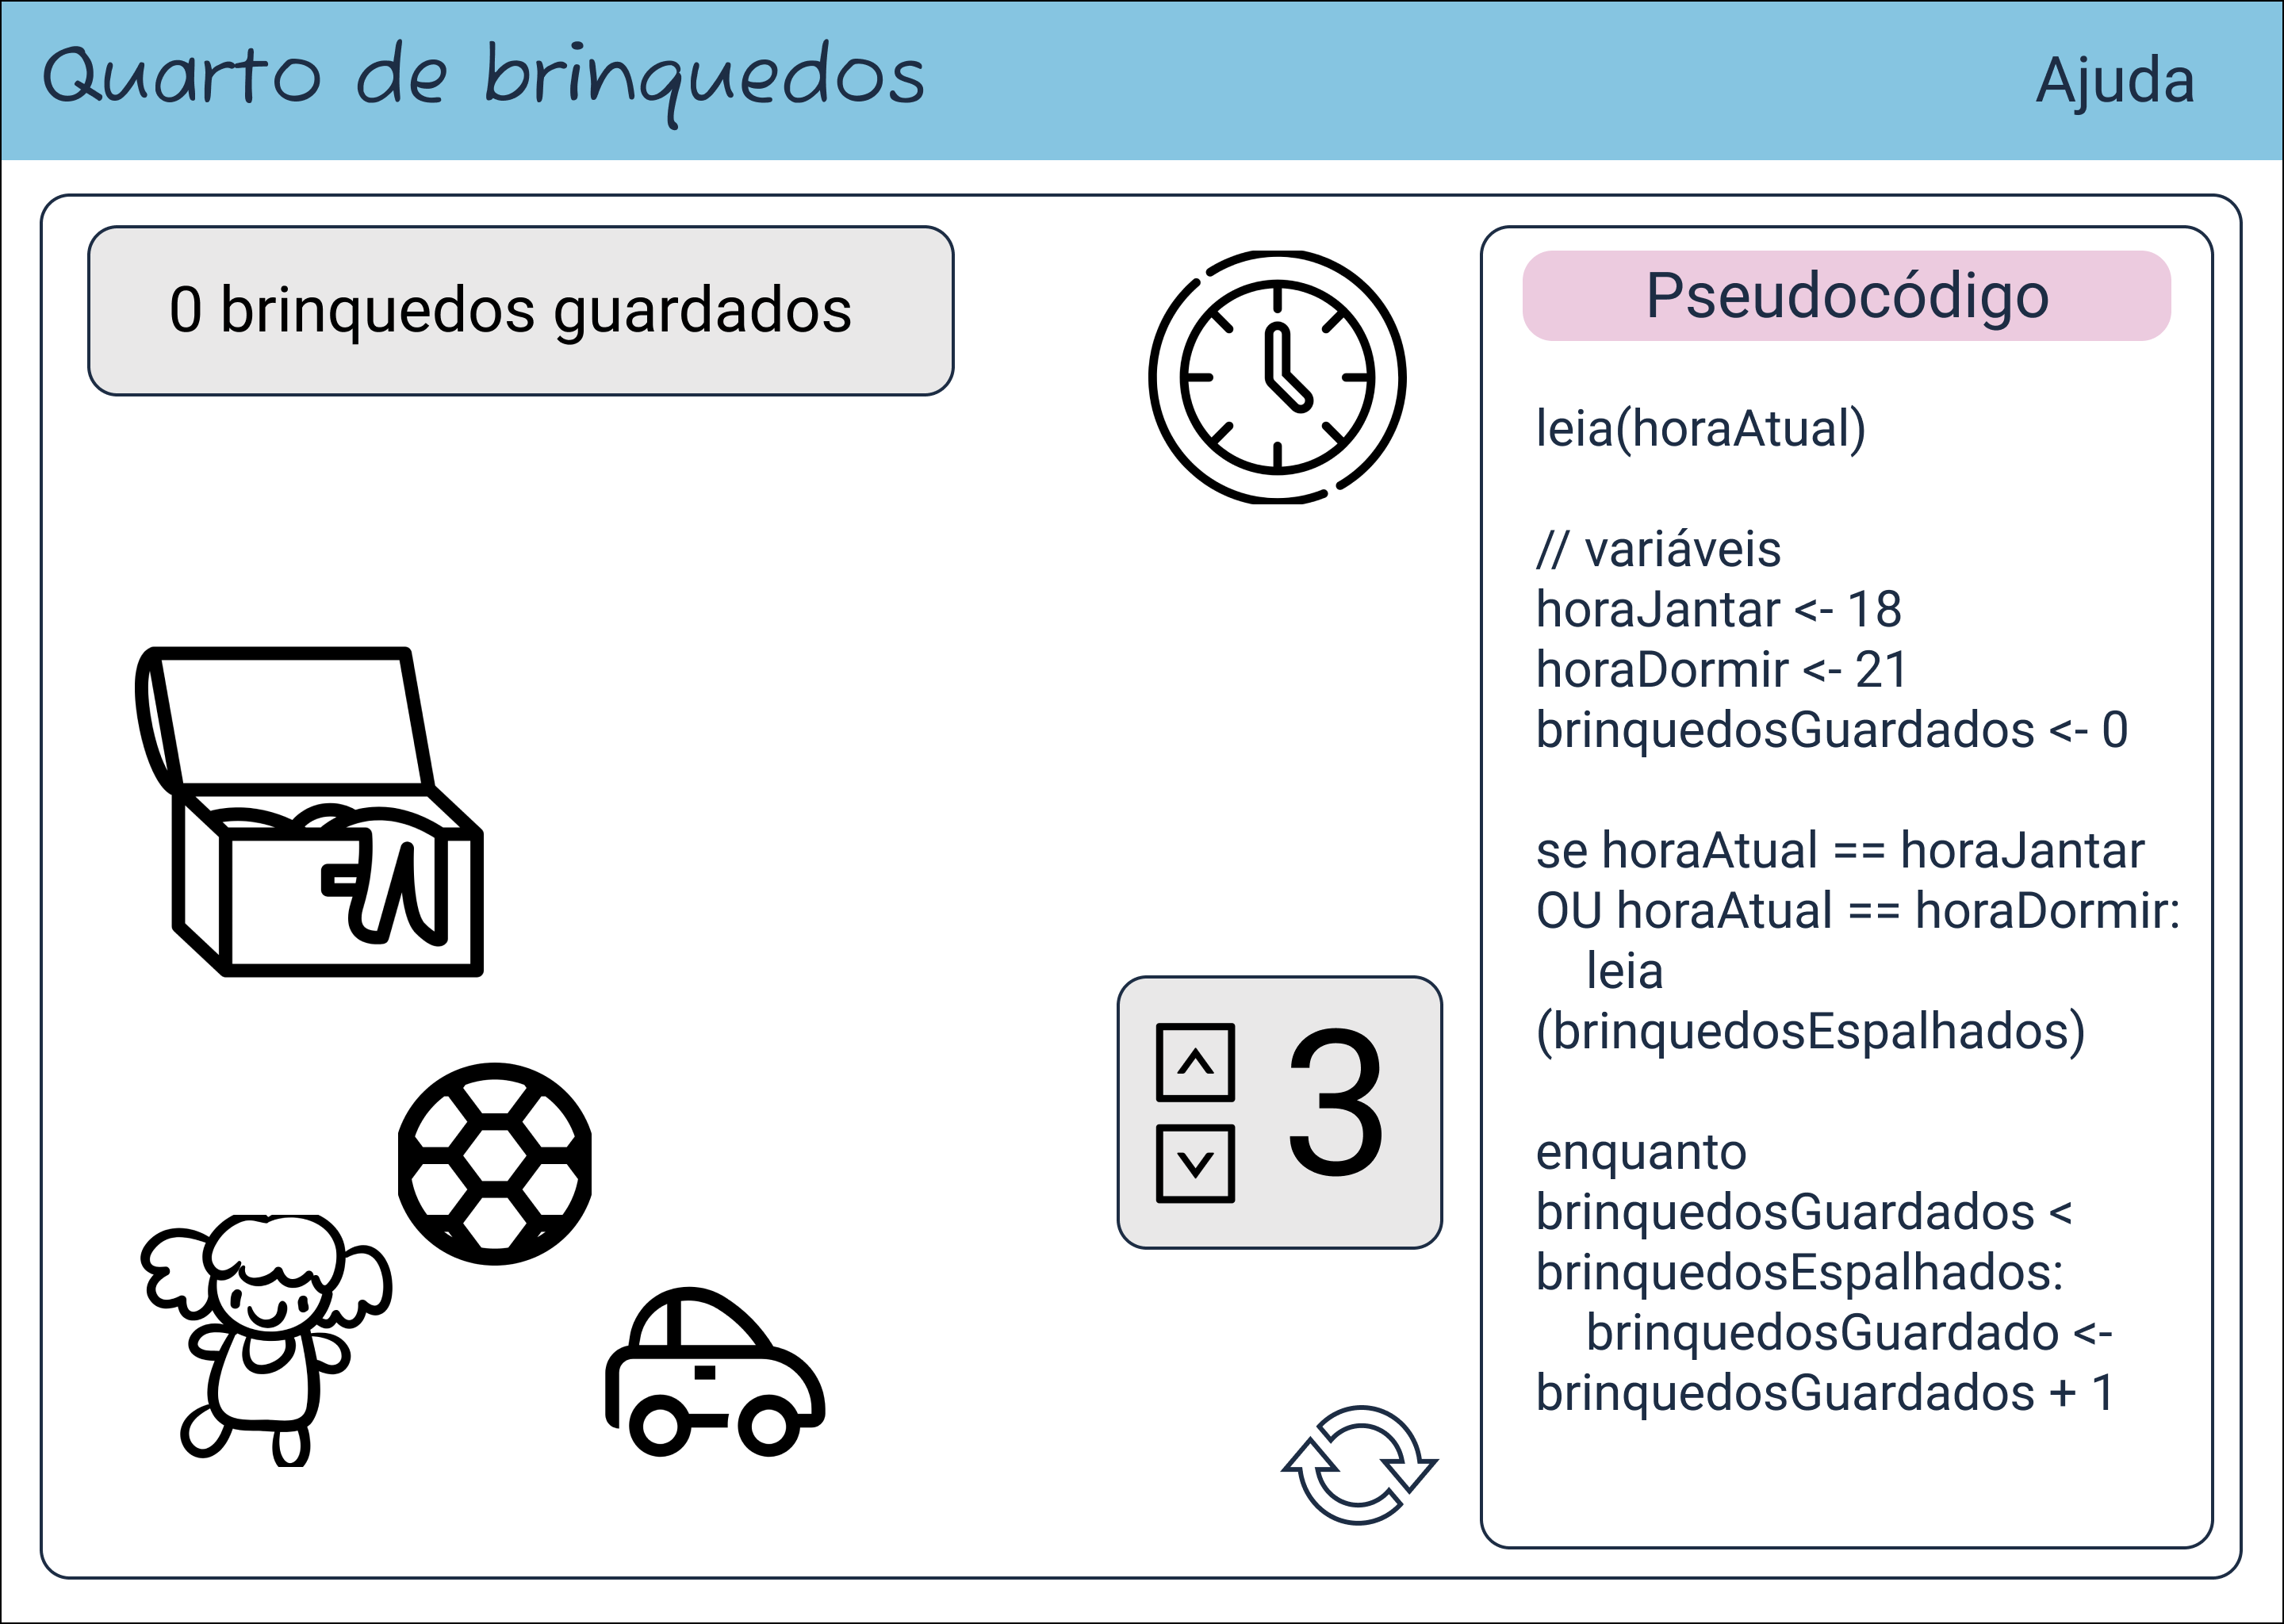
\includegraphics[scale=0.15]{prototipo_brinquedos1.png}
    \caption{Protótipo inicial da simulação \enquote{Quarto de Brinquedos}.}
    \label{figure:brinquedos1}
\end{figure}

Na Figura \ref{figure:brinquedos1}, temos um cenário de quarto de brinquedos. O protótipo da simulação apresenta elementos visuais como um relógio de parede, um baú para guardar objetos e brinquedos espalhados pelo chão. Além disso, temos dois painéis, um controle para regular a quantidade de brinquedos espalhados e um contador que mostra quantos brinquedos foram guardados. Ainda, o protótipo apresenta um pseudocódigo associado à simulação.

A princípio, a ideia dessa simulação é apresentar duas interações possíveis: alterar a hora no relógio e guardar os brinquedos no baú de forma iterativa. Com isso, queremos abordar o conceito de variáveis, principalmente, com a ação de guardar os objetos em um contêiner; de entrada, com a informação recebida através da interação com o usuário ao alterar o horário; de operadores, na comparação de expressões simples e complexas com conectivos lógicos, e na operação de adição contida na ação de guardar os brinquedos; de condicionais, verificando se é o momento de organizar o quarto; e de laços de repetição, repetindo a ação de guardar cada objeto até que o quarto esteja organizado.

\begin{figure}[h!]
    \centering
    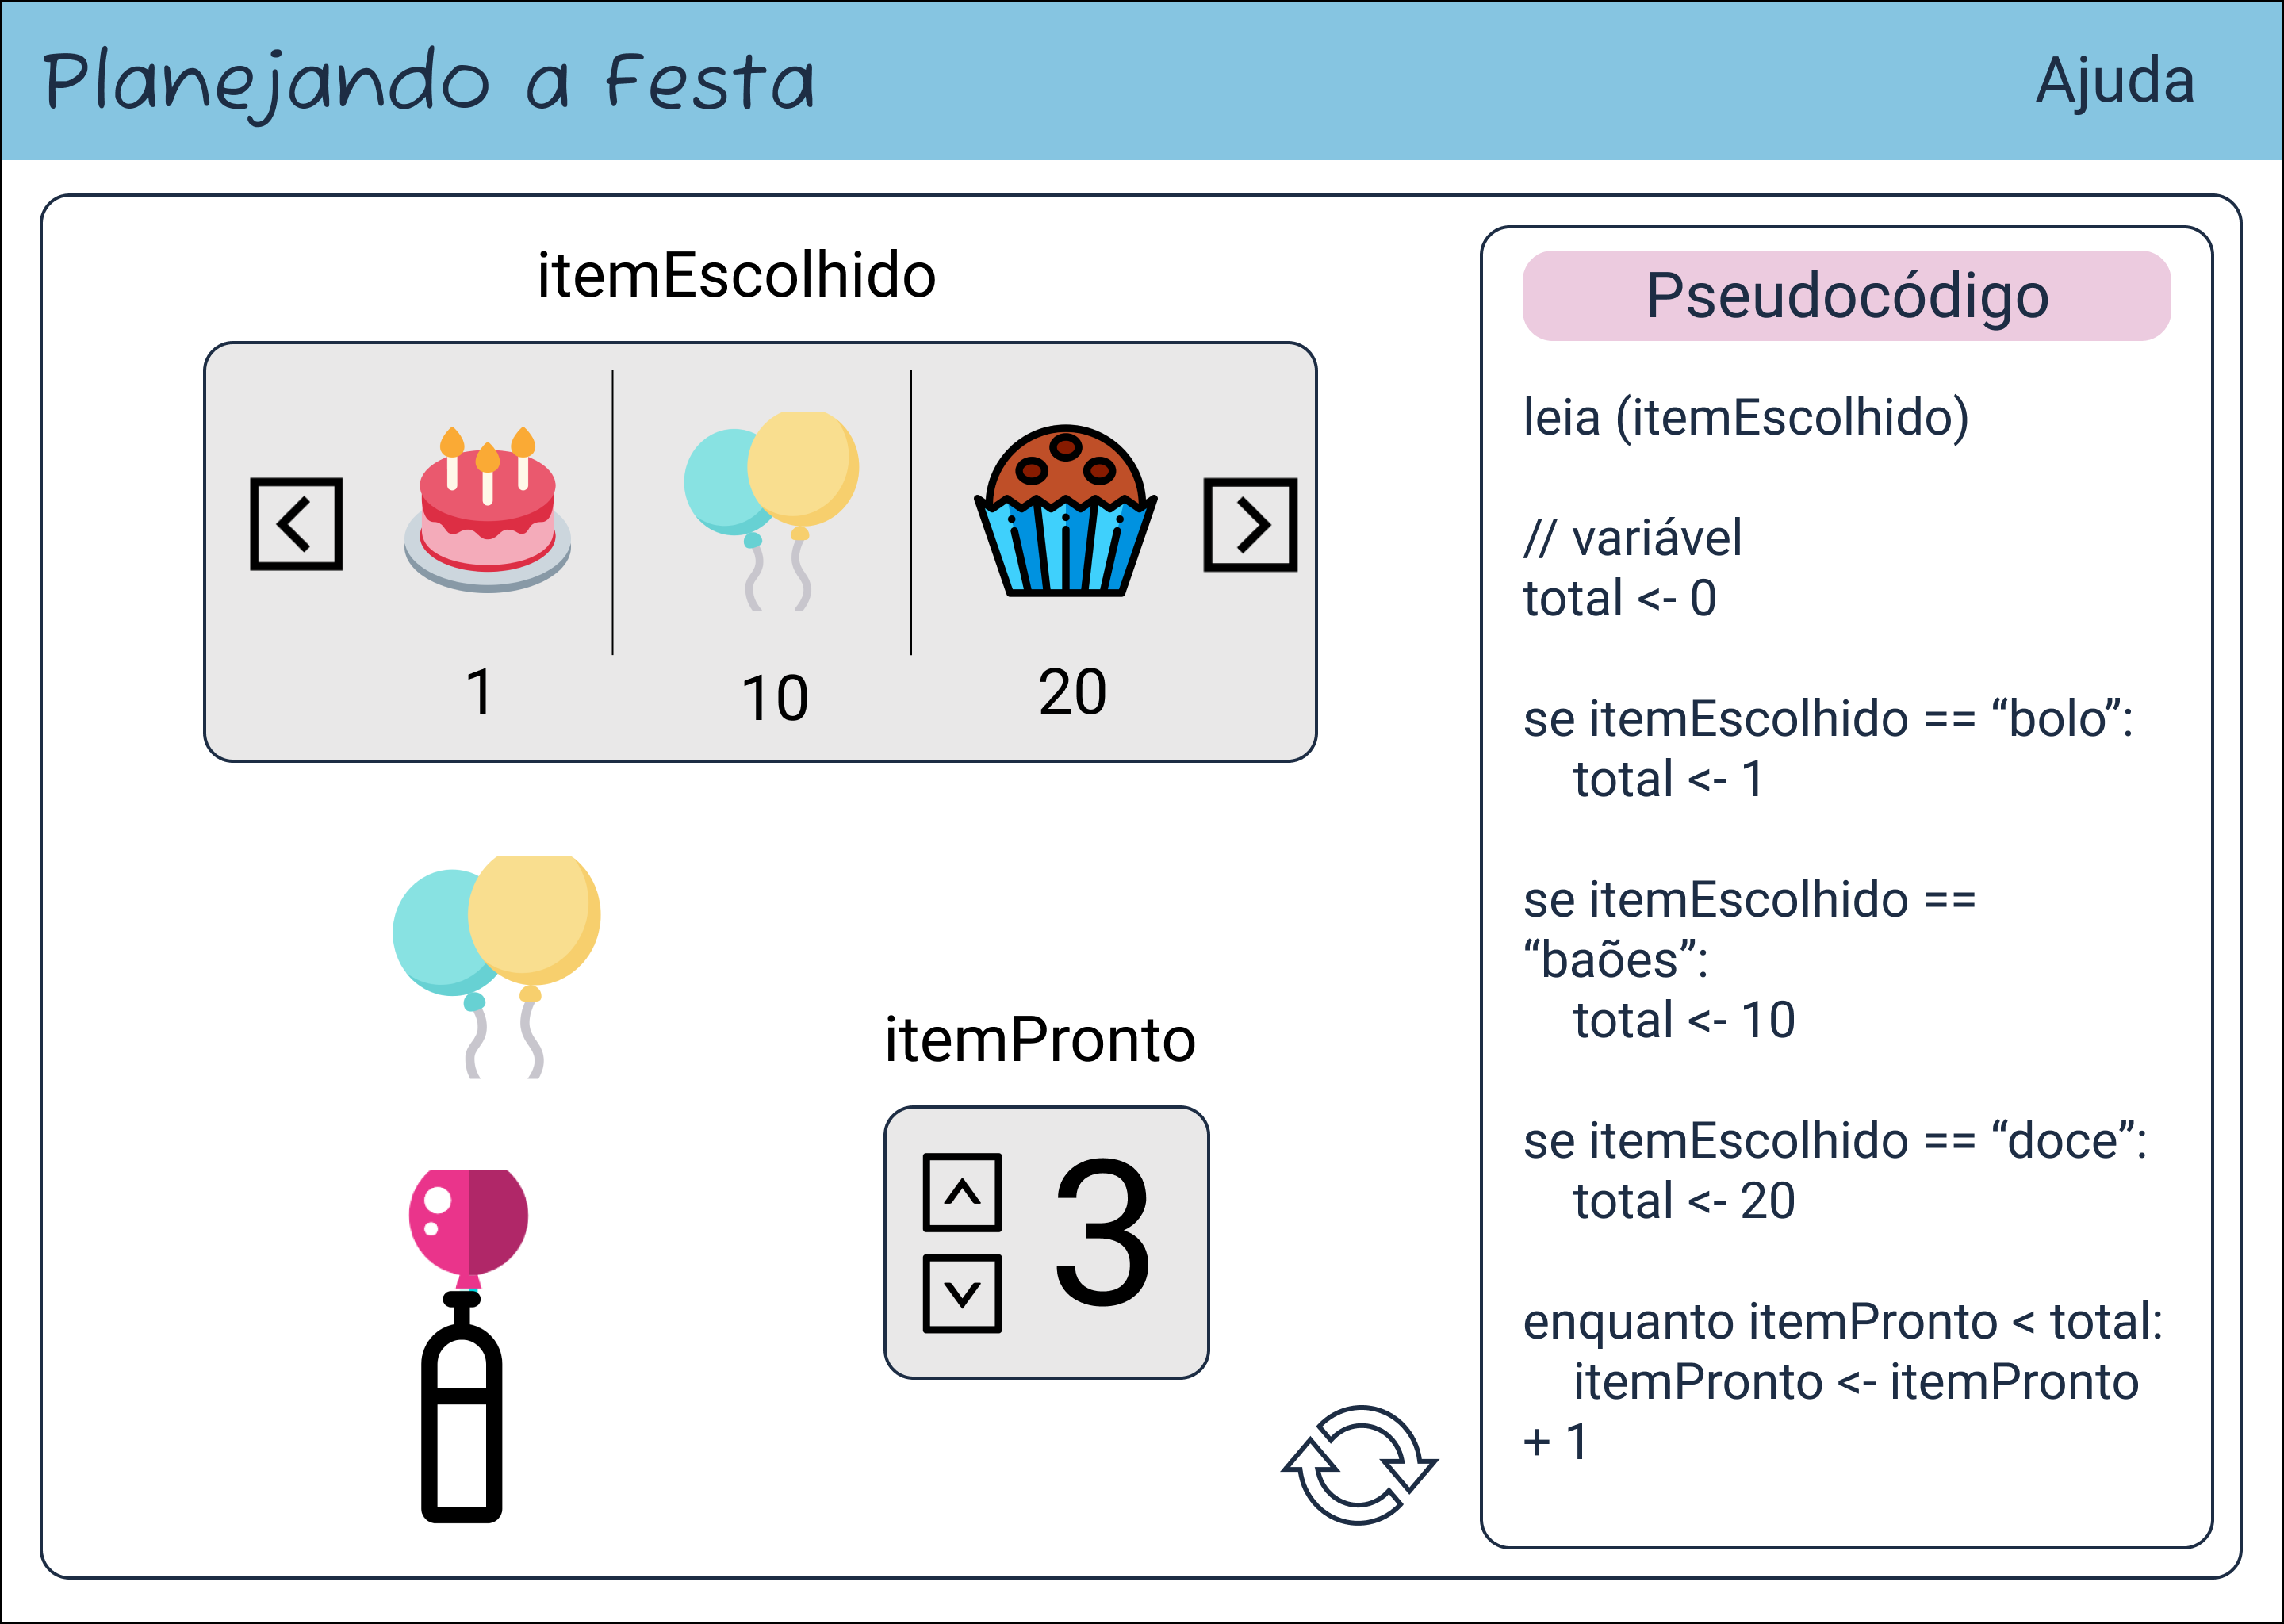
\includegraphics[scale=0.15]{prototipo_festa1.png}
    \caption{Protótipo inicial da simulação \enquote{Planejando a Festa}.}
    \label{figure:festa1}
\end{figure}

A Figura \ref{figure:festa1} apresenta um cenário de planejamento de uma festa. Nele há elementos visuais que representam itens que podem ser escolhidos para incorporar uma festa de aniversário. Ademais, temos um contador que mostra quantos itens referentes ao escolhido já estão preparados. Nessa simulação, o usuário pode ter duas interações: escolher um item para a festa e \enquote{prepará-lo} (incrementar um determinado item) até estar completo. Deste modo, nesse cenário, abordamos os conceitos de variáveis, por meio do total de objetos que devemos ter de acordo com a escolha do item; de entrada, a partir da escolha de um item para a festa; de operadores, na comparação de expressões simples, e na operação de adição contida na ação de preparar um item; de condicionais, verificando qual item foi escolhido; e de laços de repetição, conforme incremento dos objetos até atingirem o total de acordo com cada elemento.

Com os protótipos iniciais projetados, foram realizadas algumas mudanças antes de apresentá-los, conforme sugestões da professora Kelly Braghetto. As Figuras \ref{figure:brinquedos2} e \ref{figure:festa2} mostram as alterações sugeridas para os artefatos.

\begin{figure}[h!]
    \centering
    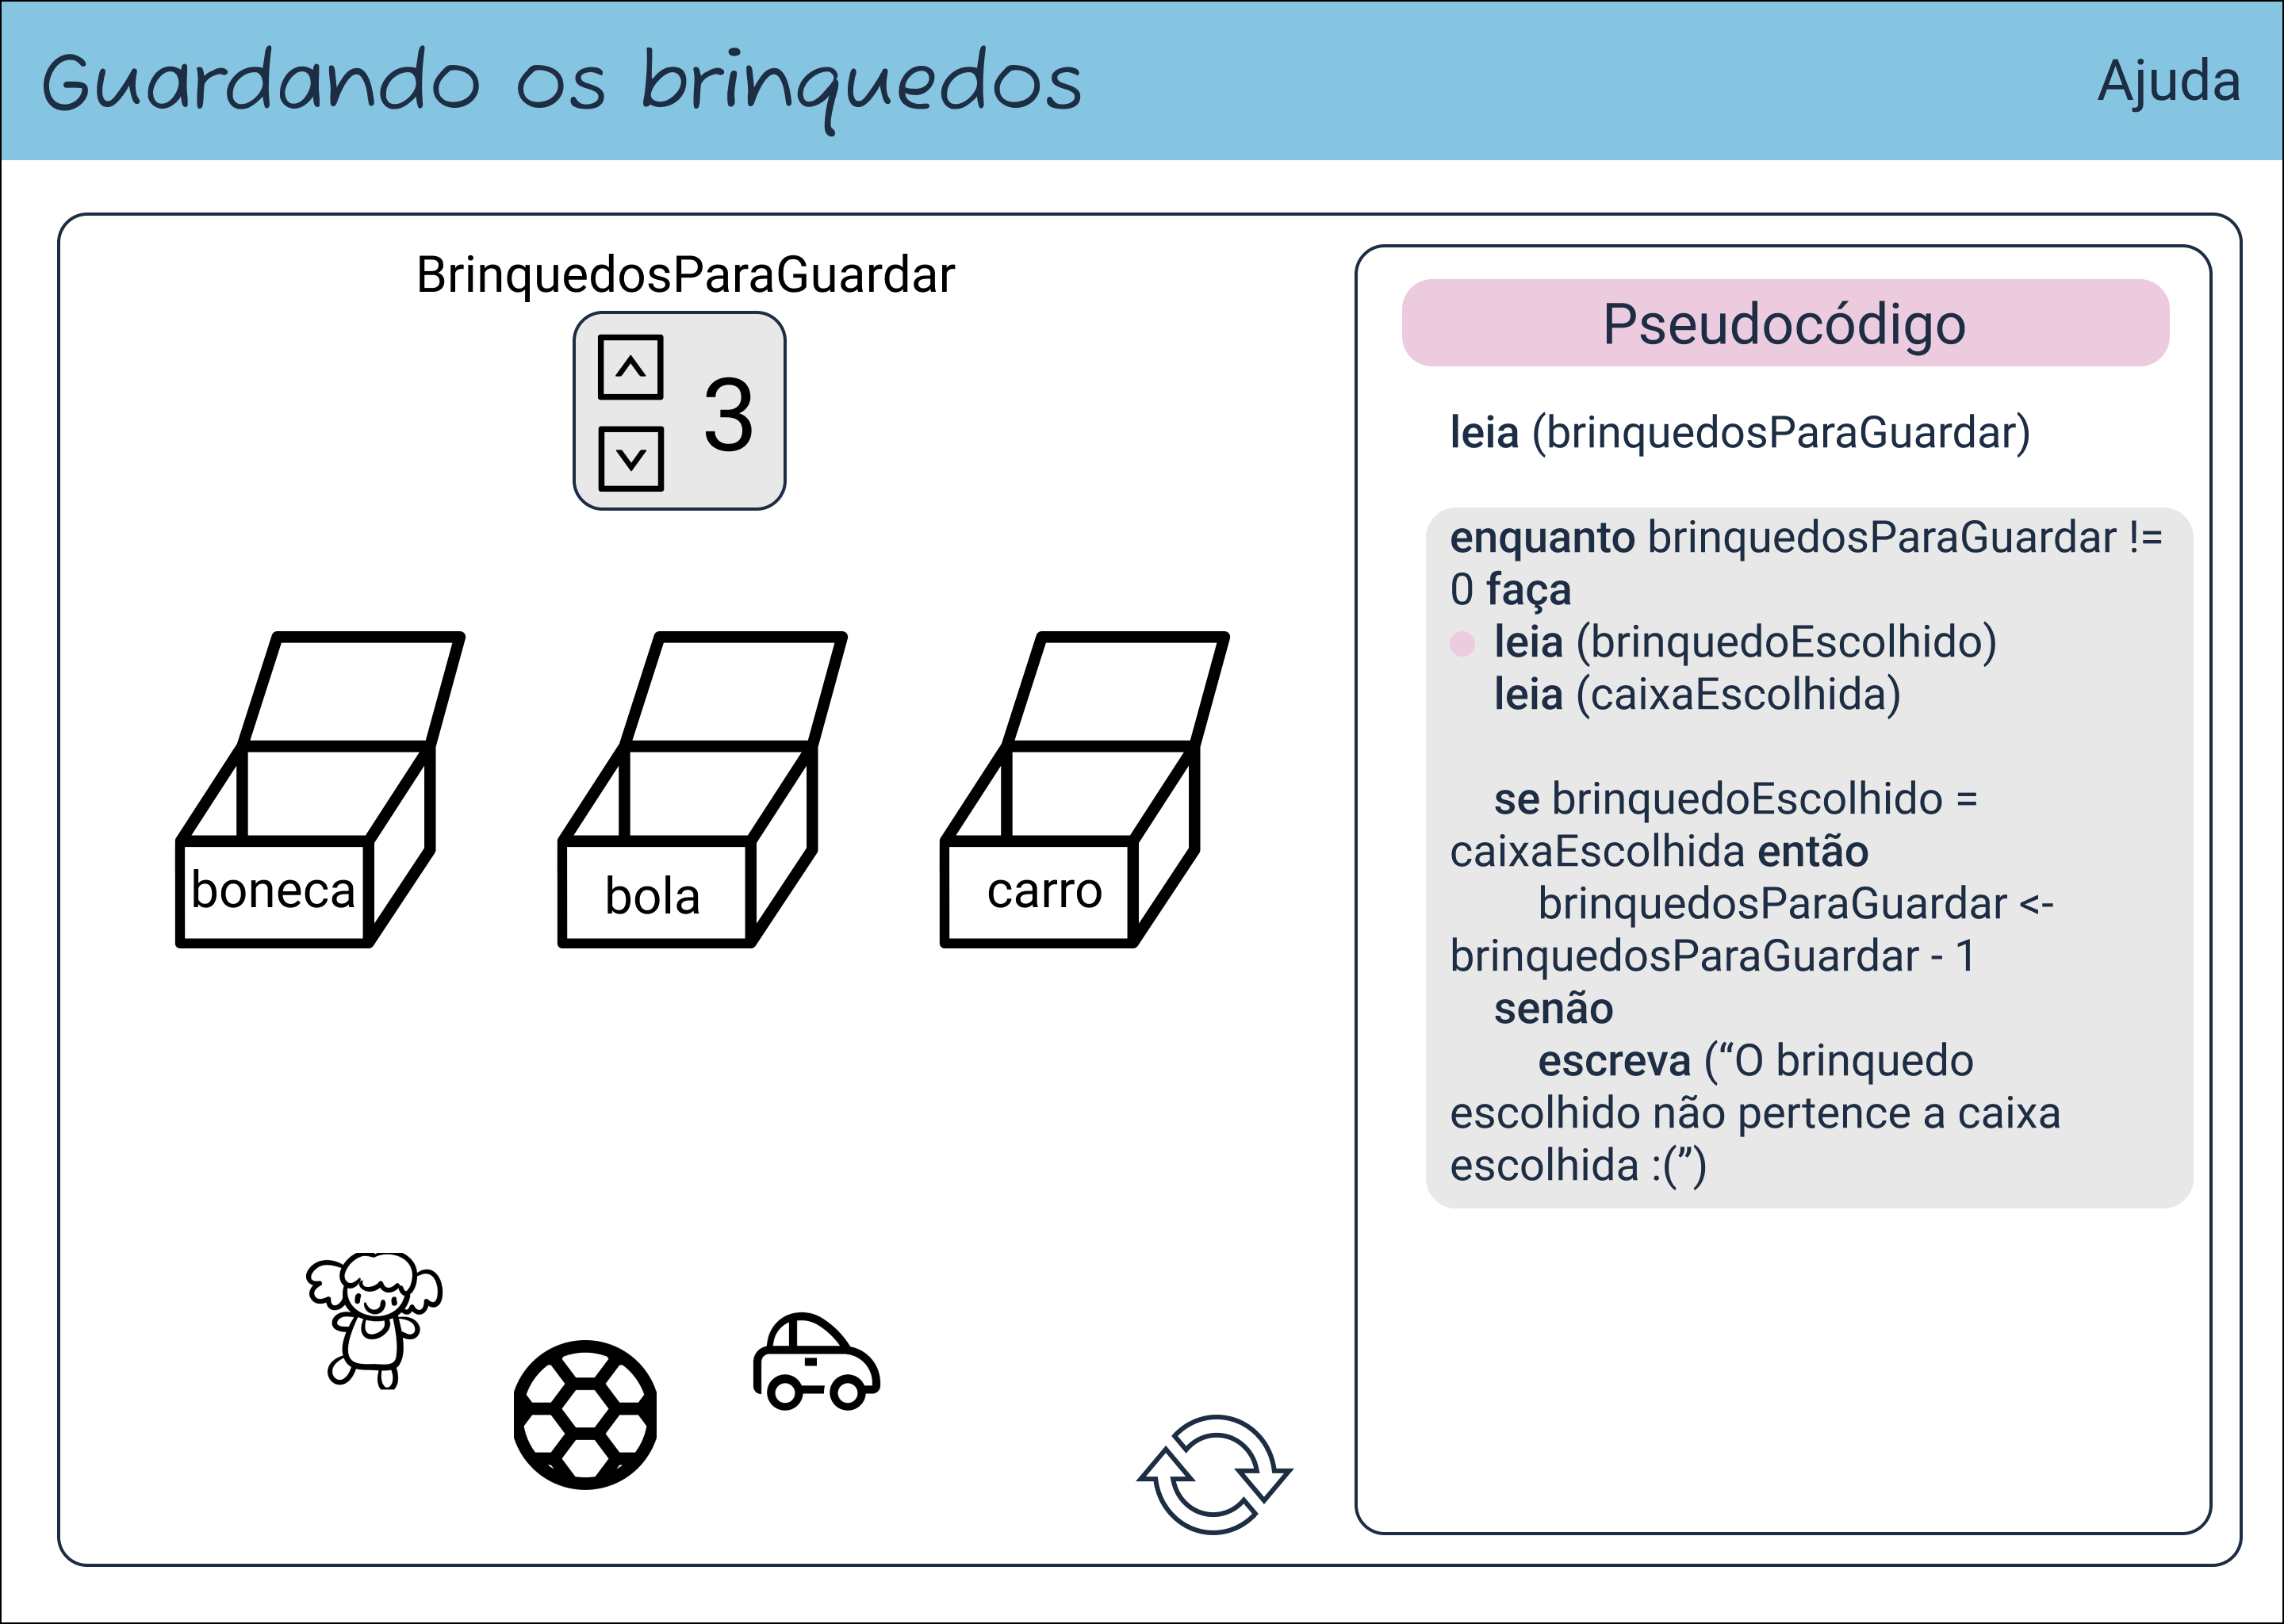
\includegraphics[scale=0.15]{prototipo_brinquedos2.png}
    \caption{Protótipo da simulação \enquote{Guardando os Brinquedos} após validação.}
    \label{figure:brinquedos2}
\end{figure}

\begin{figure}[h!]
    \centering
    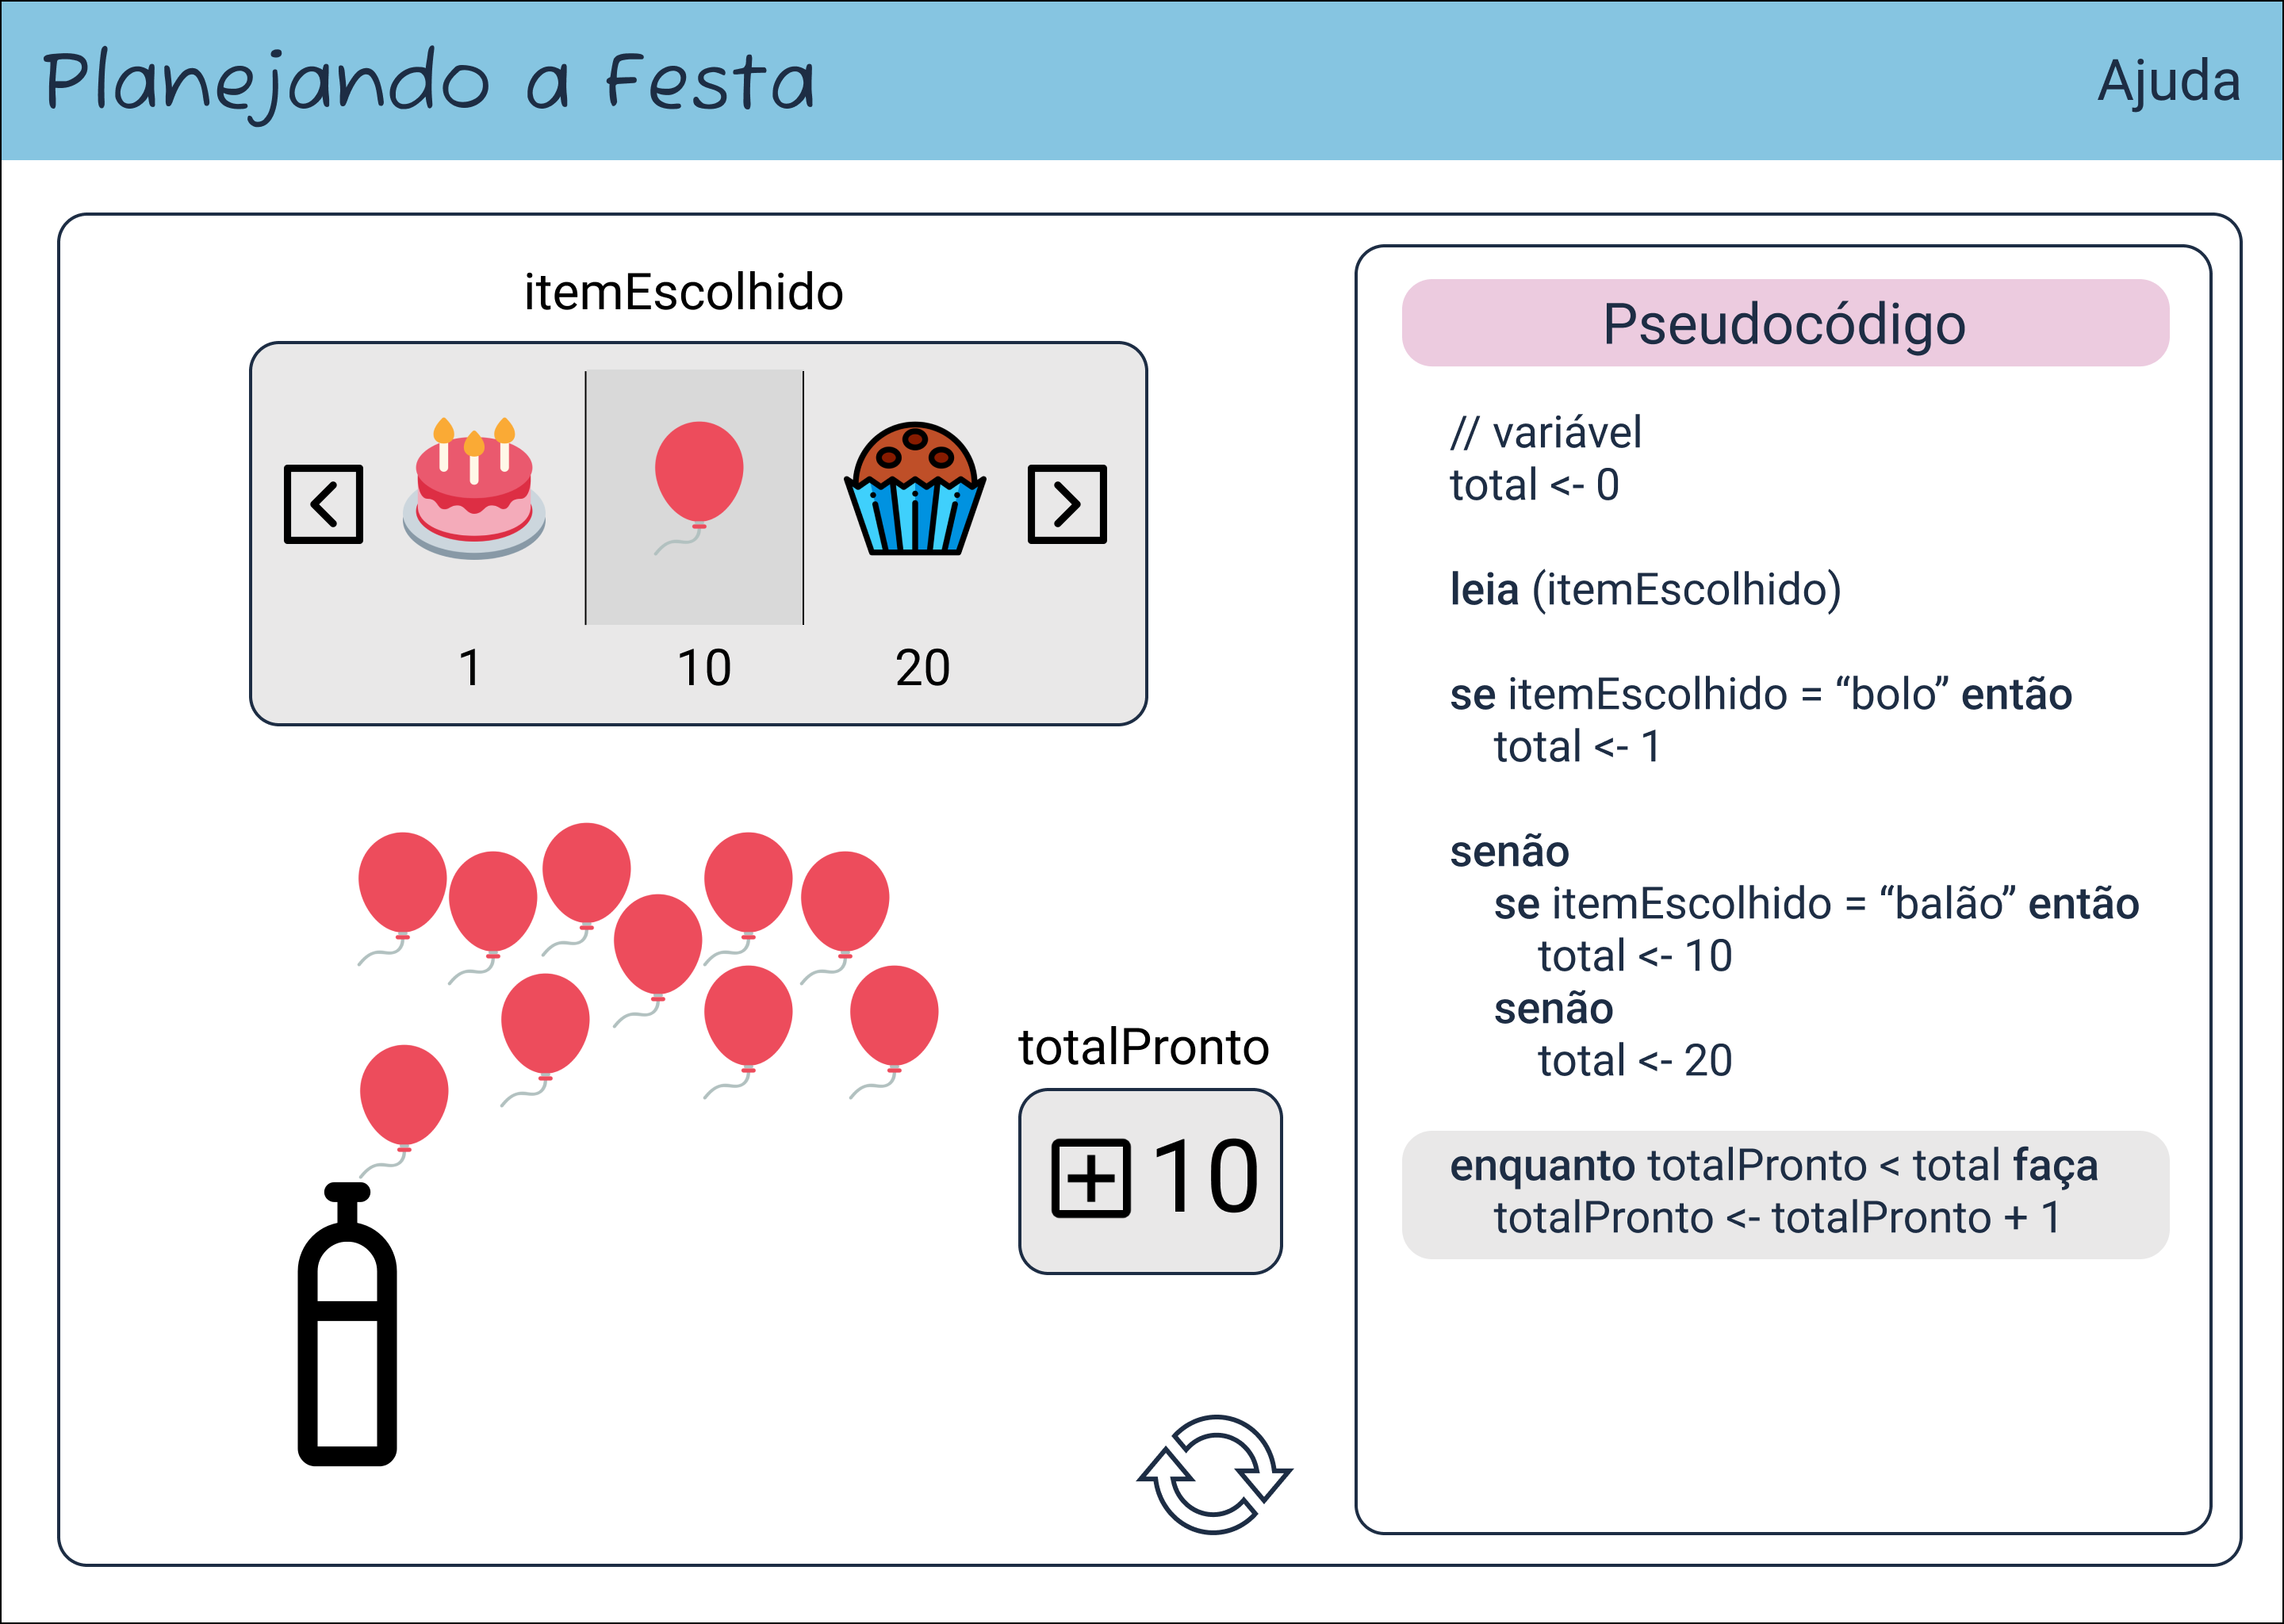
\includegraphics[scale=0.15]{prototipo_festa2.png}
    \caption{Protótipo da simulação \enquote{Planejando a Festa} após validação.}
    \label{figure:festa2}
\end{figure}

Na Figura \ref{figure:brinquedos2} podemos observar a nova simulação \enquote{Guardando os Brinquedos}, que teve sua lógica modificada para simplificar as interações com os elementos visuais e melhorar a usabilidade. Nele, há um contador que permite selecionar até três brinquedos para guardar em suas respectivas caixas. As interações possíveis nessa simulação são: incrementar o contador para escolher quantos brinquedos guardar e, após esta escolha, escolher brinquedo e caixa correspondente. A cada brinquedo guardado corretamente, o valor do contador deve ser subtraído de um. Nesse cenário, abordamos os conceitos de variáveis, na quantidade de brinquedos para guardar e nos itens (brinquedo e caixa) escolhidos; de entrada e saída, na leituras das variáveis e na escrita da mensagem quando o brinquedo e a caixa escolhida não correspondem; de operadores, na comparação de expressões simples e na operação de subtração contida na ação de guardar os brinquedos; de condicionais, verificando se o brinquedo e a caixa escolhida correspondem; e de laços de repetição, repetindo a ação de guardar cada objeto até não sobrar mais nenhum.

Já na nova versão da simulação \enquote{Planejando a Festa} (Figura \ref{figure:festa2}), podemos observar a mudança no controle do incremento do contador que indica a quantidade de itens totais prontos. Além disso, no geral, as sugestões implementadas nos protótipos envolveram a melhoria nos nomes das variáveis, a incorporação do conceito de saída e o destaque na parte do pseudocódigo em que está ocorrendo a interação na simulação.

Em seguida, em conversas com os avaliadores, foi possível obter \textit{feedbacks} para verificar a usabilidade e utilidade do MVP a partir dos protótipos projetados, possibilitando o refinamento deles e a escolha de um artefato para implementação. A simulação \enquote{Planejando a Festa} se mostrou mais interessante e com maiores possibilidades de interações e, por isso, foi escolhida como artefato a ser implementado. Ademais, o público alvo definido para a aplicação do MVP foram crianças no Ensino Fundamental II, a partir do 6° ano.

As demais sugestões recebidas pelos avaliadores levaram em conta, portanto, o protótipo escolhido e foram aplicadas diretamente na implementação do artefato. Dessa forma, a lógica da simulação \enquote{Planejando a Festa} foi alterada para melhorar a sua usabilidade e as interações com os elementos visuais. No Capítulo~\ref{cap_mvp}, descrevemos os detalhes da implementação com as modificações realizadas.

%!TeX root=../tese.tex
%("dica" para o editor de texto: este arquivo é parte de um documento maior)
% para saber mais: https://tex.stackexchange.com/q/78101

\chapter{Implementação da simulação} 
\label{cap_mvp}

O MVP da ferramenta de simulações interativas de conceitos de lógica de programação está disponível no link: \url{https://mariliatd.github.io/logic-sims-mvp/}. A tela inicial da simulação \enquote{Planejando a Festa} pode ser observada na Figura \ref{figure:tela_inicial}. Ela apresenta uma barra de navegação no topo da página, com o nome da simulação e um link de \enquote{ajuda}, o qual abre um diálogo contendo descrições do conceitos de programação abordados. Abaixo dela, há o espaço da simulação que, inicialmente, apresenta um quadro com informações sobre a ferramenta, e o espaço do pseudocódigo à direita.

\begin{figure}[h!]
    \centering
    \setlength{\fboxrule}{0.1pt} % espessura da borda da figura
    \fbox{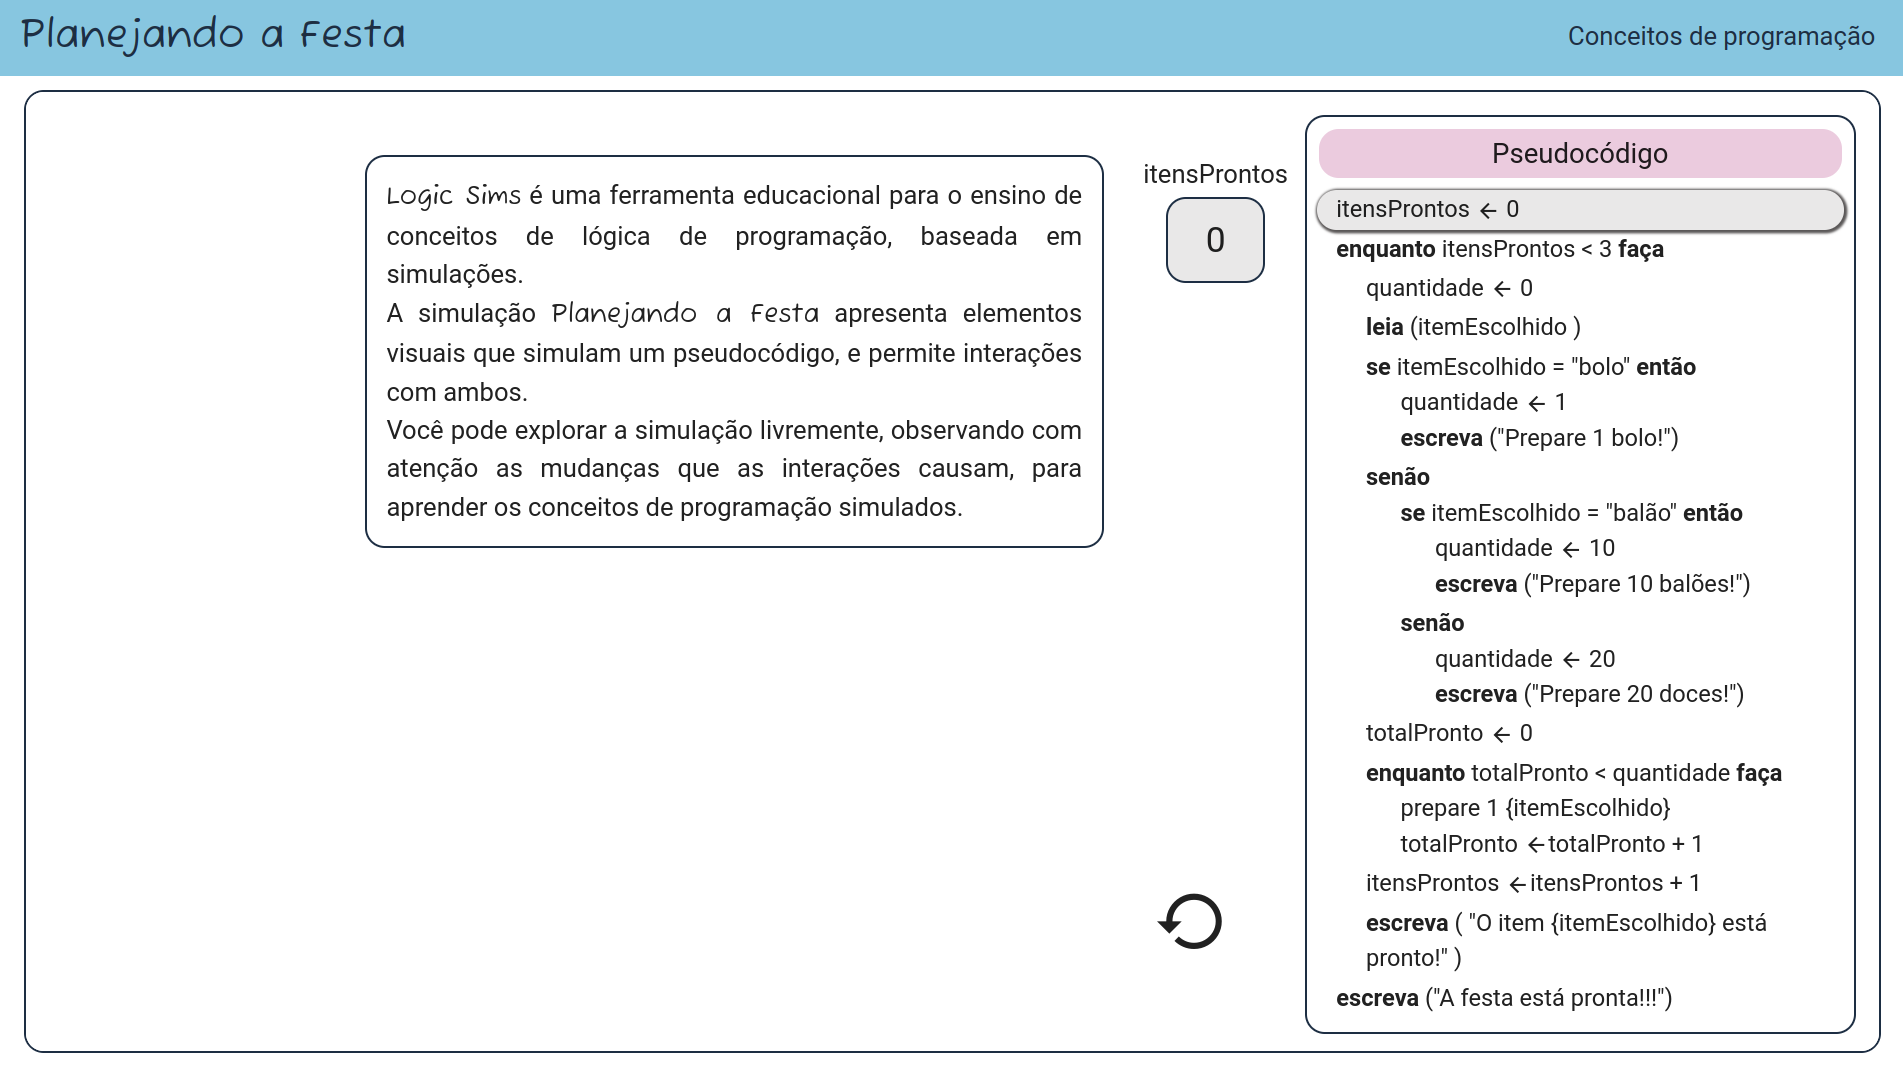
\includegraphics[scale=0.22]{tela_inicial_mvp.png}}
    \caption{Tela inicial do MVP da simulação \enquote{Planejando a Festa}.}
    \label{figure:tela_inicial}
\end{figure}

Nessa tela, é possível visualizar algumas das alterações sugeridas na etapa de validação dos protótipos. Essa nova versão da simulação também permite interações com o pseudocódigo, o qual tem as linhas destacadas com uma borda com uma animação que pisca quando é necessário interagir com ela. Esse recurso foi implementado para facilitar a visualização da \enquote{execução} de cada passo do pseudocódigo, o qual foi modificado. Adicionamos à lógica da simulação um laço de repetição externo para realizar a iteração na preparação dos três itens disponíveis para compor a festa, que faltava no projeto do protótipo.

Assim, a simulação permite selecionar três itens em quantidades distintas e preparar cada um até atingir as quantidades correspondentes até que a festa esteja pronta. A seleção de um item pelo usuário representa a entrada ou leitura de um valor no pseudocódigo, que condiciona a quantidade de itens a serem preparados. Ao escolher um item ou finalizar o seu preparo e quando a festa está pronta são impressas mensagens na tela em uma janela representando a saída de dados no pseudocódigo, como mostra a Figura \ref{figure:saida}. 

\begin{figure}[h!]
    \centering
    \setlength{\fboxrule}{0.1pt} % espessura da borda da figura
    \fbox{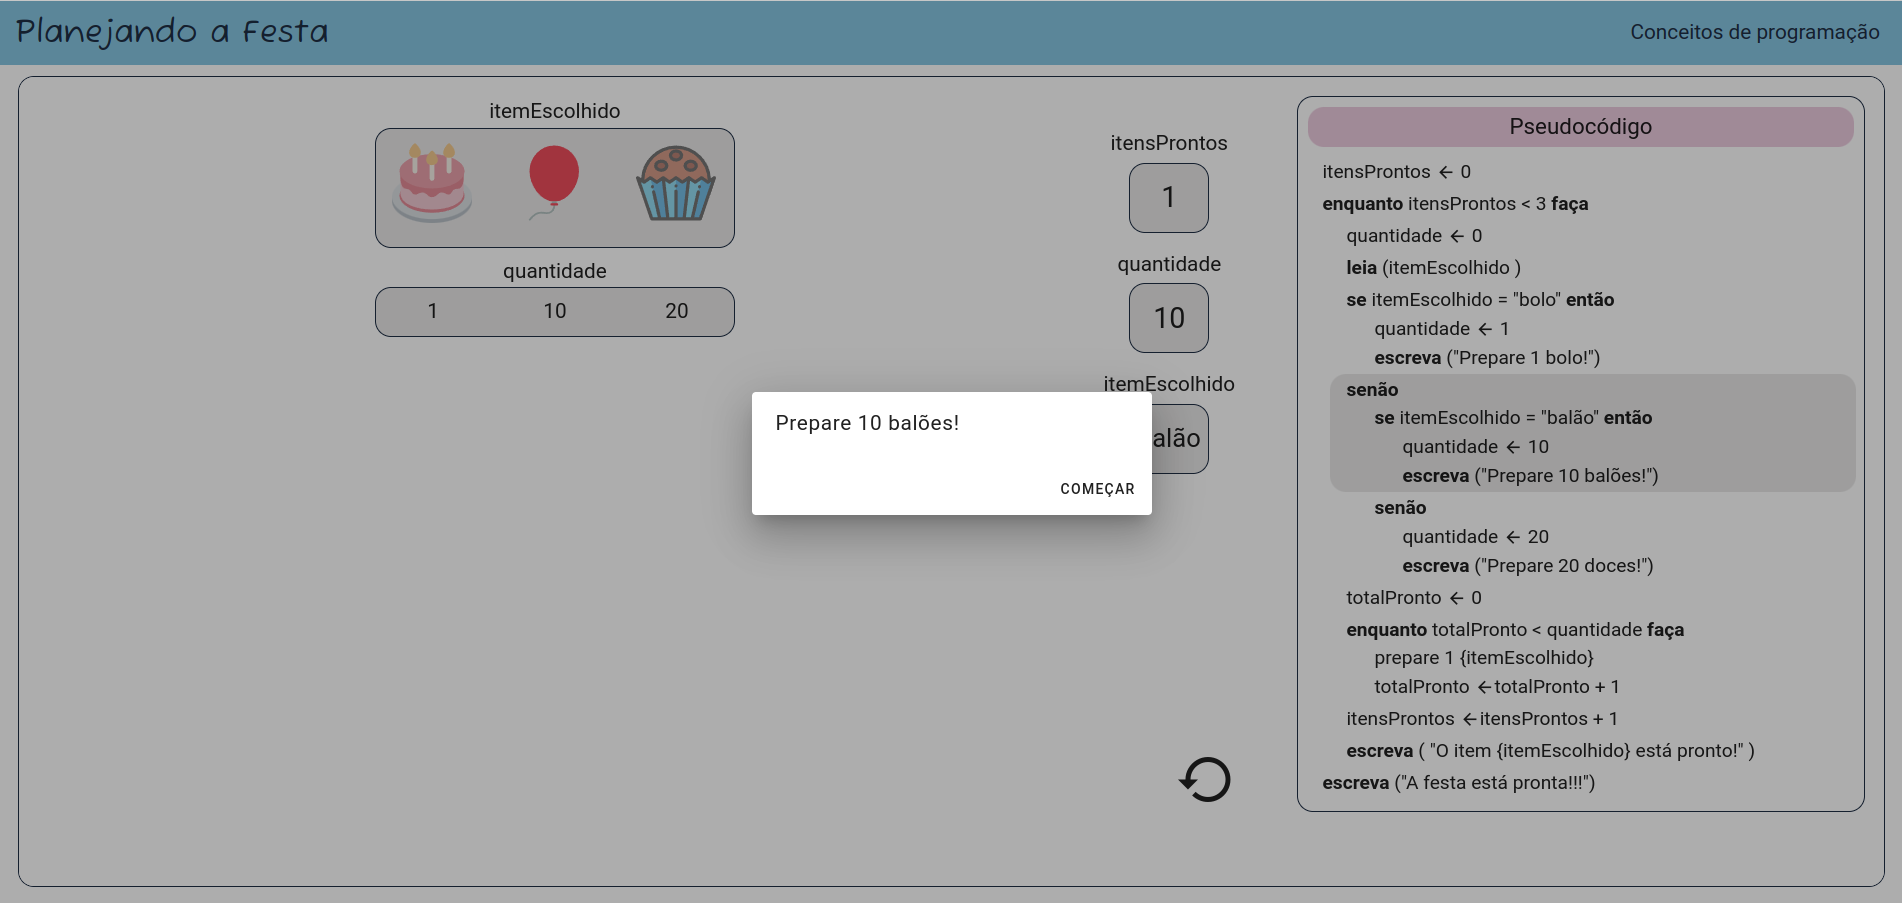
\includegraphics[scale=0.22]{saida.png}}
    \caption{Representação visual do conceito de saída com a mensagem \enquote{impressa} na tela.}
    \label{figure:saida}
\end{figure}

Quando o usuário seleciona um item para preparo, a escolha dos demais fica desabilitada, para que a interação com a simulação siga o fluxo do pseudocódigo e não permita que o usuário troque de item enquanto está dentro do laço de repetição interno, por exemplo. A Figura \ref{figure:item_escolhido} mostra o cenário em que o item \enquote{bolo} foi selecionado e os demais estão sombreados, não sendo possível clicar neles. Ainda, após o preparo de um item, este fica desabilitado para escolha na iteração seguinte, limitando o preparo dos três itens (em qualquer ordem) para finalizar o preparo da festa e a simulação.

\begin{figure}[h!]
    \centering
    \setlength{\fboxrule}{0.1pt} % espessura da borda da figura
    \fbox{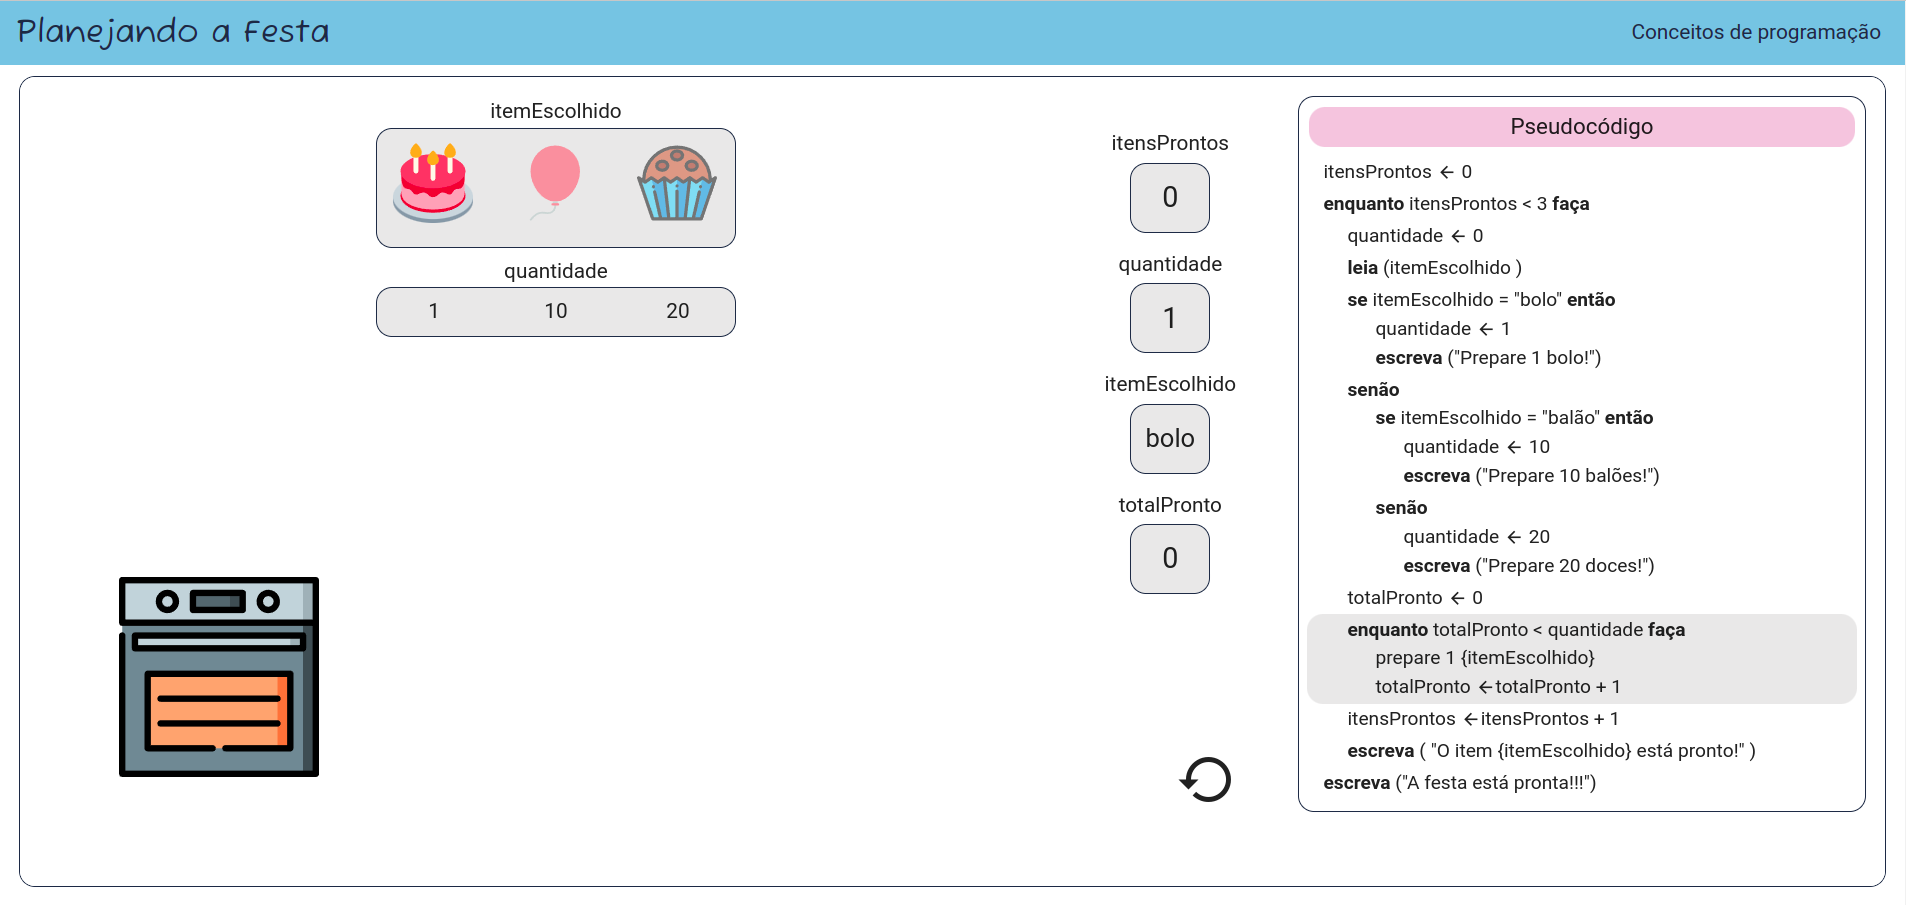
\includegraphics[scale=0.22]{item_escolhido.png}}
    \caption{Escolhendo um item na simulação \enquote{Planejando a Festa}.}
    \label{figure:item_escolhido}
\end{figure}

Na Figura \ref{figure:item_escolhido} também podemos observar que cada variável está separada em um elemento visual próprio. Além disso, removemos o controle do incremento do contador que indica a quantidade total pronta de cada item, deixando essa interação apenas nas figuras de preparo de cada item (fogão, cilindro de gás e pratos) para representar o laço de repetição interno do pseudocódigo. Ainda, adicionamos o pseudocódigo para a execução das atividades de preparo do item escolhido dentro desse laço.

Outro recurso incorporado no pseudocódigo da simulação foi a adição de cores para diferenciar os conceitos de lógica de programação, o qual é comumente utilizado nas linguagens de programação em blocos. A escolha das cores foi feita através da ferramenta Coolors\footnote{\url{coolors.co}} que além de apresentar um gerador de paleta de cores, também disponibiliza um verificador de contraste. Ela segue as Diretrizes de Acessibilidade para Conteúdo \textit{Web} (\textit{Web Content Accessibility Guidelines - WCAG}), a qual define uma série de recomendações para tornar a web mais acessível \citep{caldwell2008web}. A categorização das cores foi feita da seguinte forma:

\definecolor{variables}{HTML}{F9F1A8}
\definecolor{inputOutput}{HTML}{FFC17C}
\definecolor{operators}{HTML}{D0F4DE}
\definecolor{conditional}{HTML}{E4C1F9}
\definecolor{loop}{HTML}{A9DEF9}

\begin{itemize}
    \item \colorbox{variables}{Variáveis} (amarelo)
    \item \colorbox{inputOutput}{Entrada} e \colorbox{inputOutput}{saída} (laranja)
    \item \colorbox{operators}{Operadores} (verde)
    \item \colorbox{conditional}{Condicionais} (roxo)
    \item \colorbox{loop}{Laço de repetição} (azul)
\end{itemize}

\noindent Além disso, a simulação mostra o nome de cada conceito de lógica de programação. Esse recurso pode ser visualizado ao passar o mouse em cima de cada conceito. A Figura \ref{figure:pseudocodigo_destaque} apresenta as alterações destacadas.

\begin{figure}[h!]
    \centering
    \setlength{\fboxrule}{0.1pt} % espessura da borda da figura
    \fbox{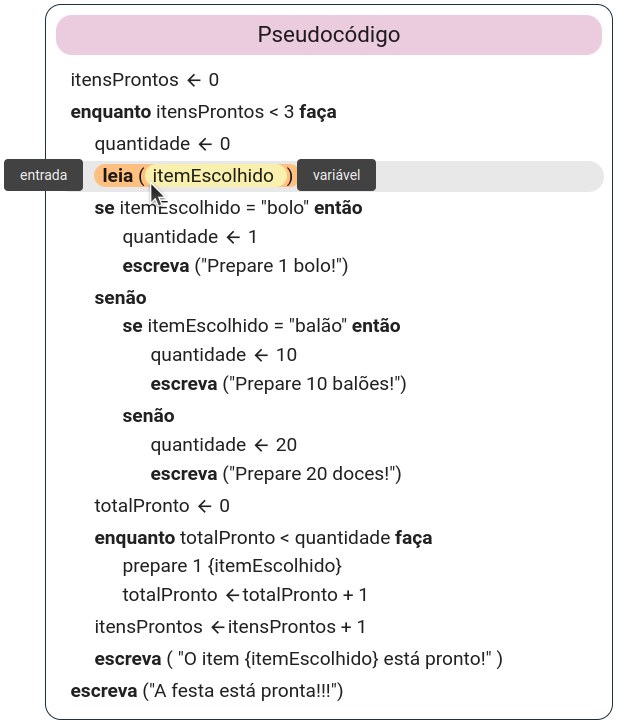
\includegraphics[scale=0.32]{pseudocodigo_destaque1.png}
    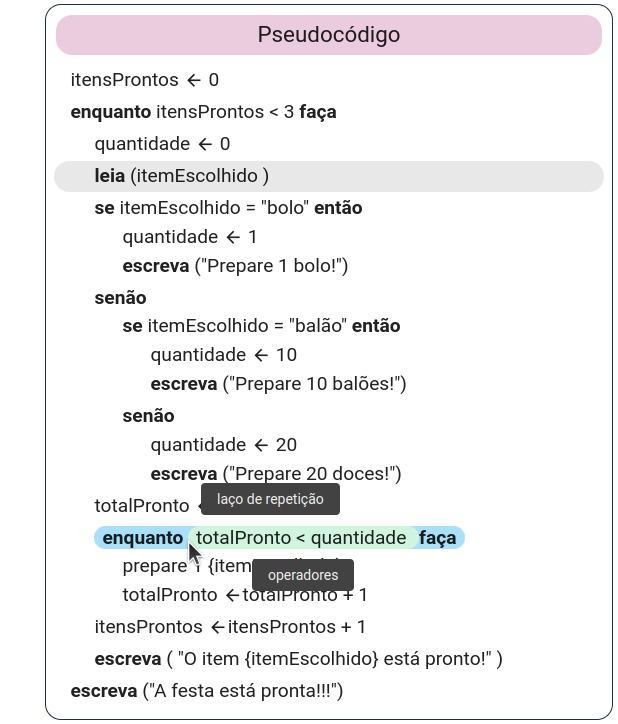
\includegraphics[scale=0.35]{pseudocodigo_destaque2.png}}
    \caption{Destaques do pseudocódigo da simulação \enquote{Planejando a Festa} mostrando a separação em cores por conceito de lógica de programação e a indicação do nome deles ao passar o mouse por cima de cada um.}
    \label{figure:pseudocodigo_destaque}
\end{figure}

Por fim, o \textit{link} para \enquote{Ajuda} na barra de navegação foi renomeado para \enquote{Conceitos de programação} e ele abre uma caixa de diálogo contendo definições de cada conceito, com figuras e exemplos (Figura \ref{figure:conceitos_programacao}). As definições contêm pseudocódigos de exemplo que seguem o esquema de cores descrito acima.

\begin{figure}[h!]
    \centering
    \setlength{\fboxrule}{0.1pt} % espessura da borda da figura
    \fbox{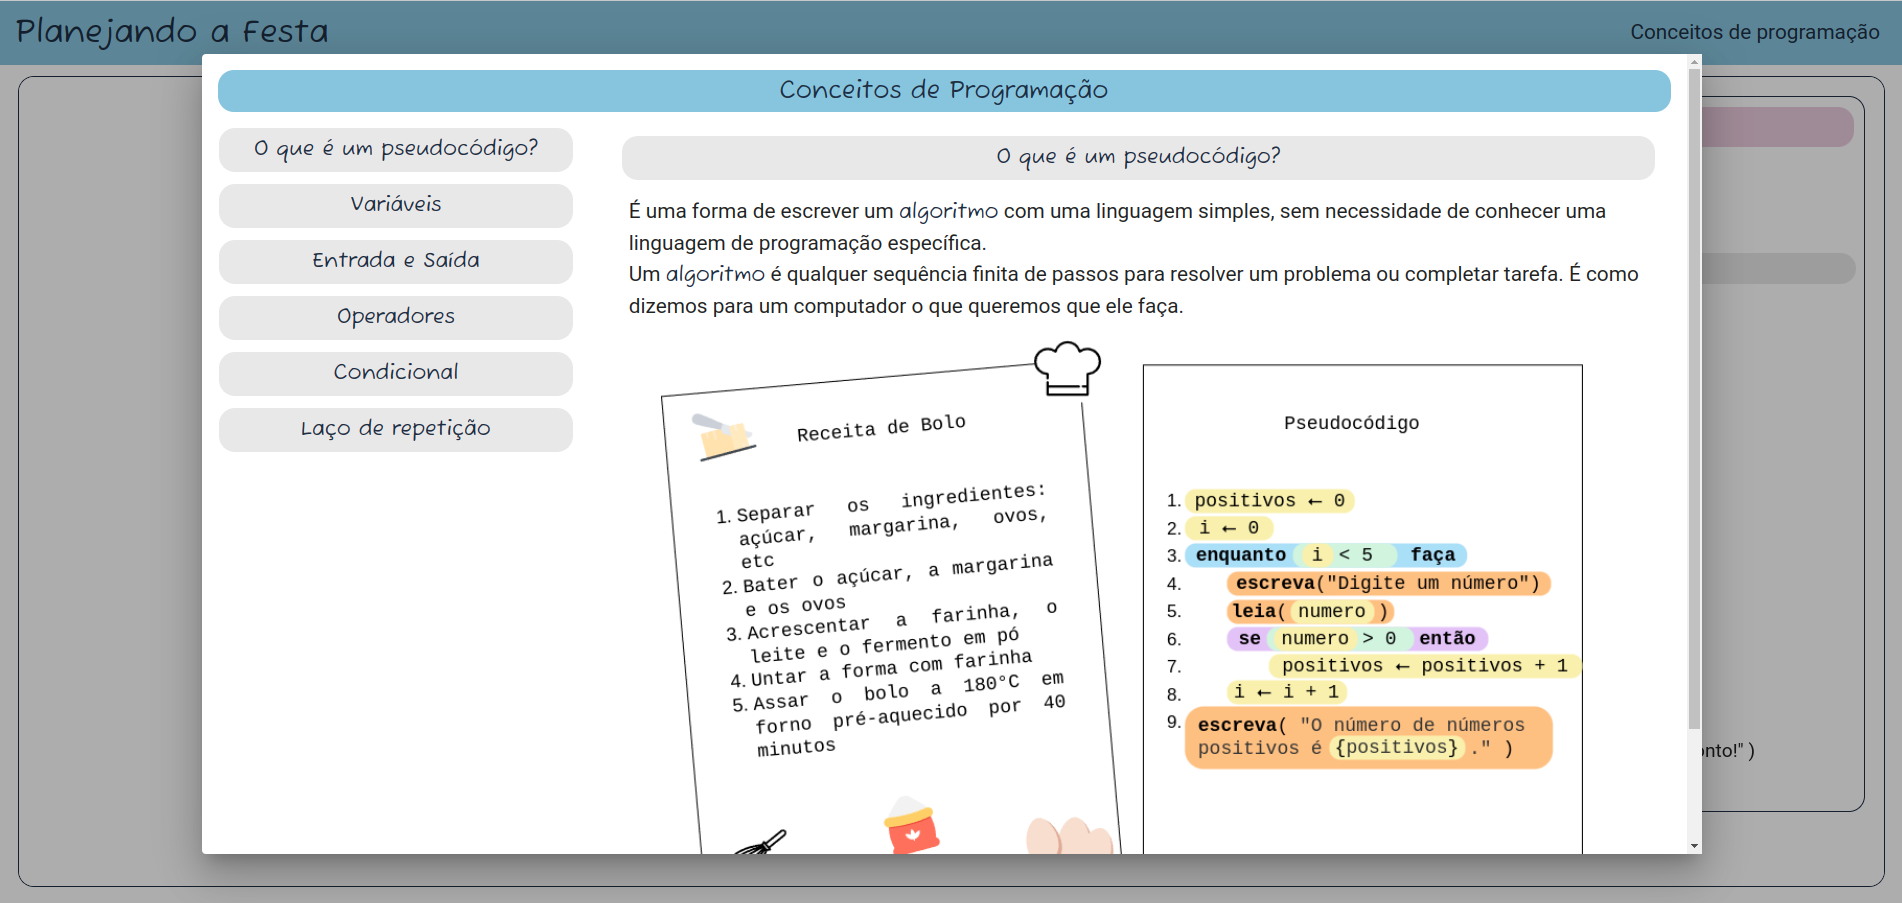
\includegraphics[scale=0.22]{conceitos_programacao.png}}
    \caption{Caixa de diálogo contendo as definições dos conceitos de lógica de programação abordados na simulação \enquote{Planejando a Festa}. O menu lateral permite a escolha de um conceito, mostrando a sua definição e exemplos ao lado.}
    \label{figure:conceitos_programacao}
\end{figure}

%!TeX root=../tese.tex
%("dica" para o editor de texto: este arquivo é parte de um documento maior)
% para saber mais: https://tex.stackexchange.com/q/78101


\chapter{Avaliação da simulação} \label{evaluation}

A avaliação da simulação por meio da escala de usabilidade (SUS) e da atividade de aprendizado foi realizada em sala de aula com os usuários finais. Para isso, realizamos uma atividade com a duração de uma aula de 50 minutos com uma turma de 26 alunos com idades entre 13 e 14 anos, do 8° ano do Ensino Fundamental II da Escola de Aplicação da Faculdade de Educação da USP (FEUSP). Durante a aula, contamos com o apoio do professor Henri Silva, que leciona matemática para a turma. 

A atividade realizada em aula foi dividida em três partes: na primeira, apresentamos um exemplo de pseudocódigo e código em Python de um programa que, dados cinco números de entrada, calcula a quantidade de números pares e de números ímpares; na segunda parte, os alunos exploraram o MVP com a simulação de forma livre; e na terceira, eles preencheram dois formulários, o da escala de usabilidade e o da atividade de aprendizado, nessa ordem.

As 10 afirmações adaptadas do SUS e traduzidas para o português, apresentadas no formulário de usabilidade, estão enumeradas a seguir, enquanto a escala visual de Likert utilizada é mostrada na Figura \ref{figure:likert_forms}.

\begin{enumerate}
    \item Eu gostaria de explorar mais a simulação.
    \item Eu fiquei confuso(a) muitas vezes enquanto explorava a simulação.
    \item Eu achei que a simulação foi fácil de usar.
    \item Eu precisaria de ajuda para conseguir explorar a simulação.
    \item Eu sabia o que era preciso fazer quando explorei a simulação.
    \item Algumas coisas que eu tive que fazer enquanto explorava a simulação não fizeram sentido.
    \item Eu acho que a maioria dos meus amigos podem aprender a usar a simulação muito rápido.
    \item Algumas das coisas que eu tive que fazer para explorar a simulação foram estranhas.
    \item Eu me senti confiante enquanto explorava a simulação.
    \item Eu tive que aprender muitas coisas antes de explorar a simulação.
\end{enumerate}

\begin{figure}[h!]
    \centering
    \setlength{\fboxrule}{0.1pt} % espessura da borda da figura
    \fbox{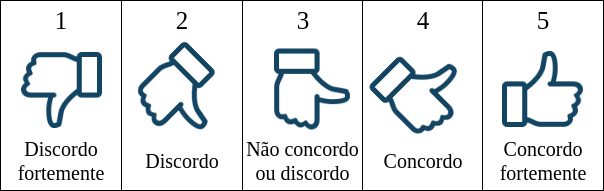
\includegraphics[scale=0.5]{escalaLikertformulario.png}}
    \caption{Representação visual da escala de Likert utilizada no formulário de usabilidade.}
    \label{figure:likert_forms}
\end{figure}

Ainda, ao final do formulário foram feitas duas perguntas dissertativas sobre o que o usuário mais gostou na simulação e o que menos gostou, além de um espaço adicional para deixar quaisquer comentários ou sugestões sobre ela.

A atividade de aprendizado foi dividida em duas partes com 6 perguntas cada. Em cada pergunta, foi apresentado um trecho do pseudocódigo com um ou mais conceitos de lógica de programação e foi pedido para selecionar a opção que melhor representasse aquele pedaço de pseudocódigo, entre as seguintes opções: variáveis, entrada, saída, operadores, condicional e laço de repetição. A primeira parte da atividade continha perguntas sobre o pseudocódigo da simulação \enquote{Planejando a Festa}, explorada pelos estudantes. A Figura \ref{figure:atividade_festa} mostra os trechos de pseudocódigo apresentados em cada questão. A segunda parte era referente à simulação \enquote{Guardando os Brinquedos}, a qual foi apresentada no formulário, para fornecer contexto para as questões, por meio de uma imagem (Figura \ref{figure:brinquedos_forms}). Essa simulação é uma versão modificada da criada na etapa de projeto dos artefatos, apresentada no Capítulo \ref{prototypes}. A Figura \ref{figure:atividade_brinquedos} mostra os pedaços de pseudocódigo utilizados nessas questões.

\begin{figure}[h!]
    \centering
    \begin{subfigure}[t]{0.5\textwidth}
        \centering
        \setlength{\fboxrule}{0.1pt} % espessura da borda da figura
        \fbox{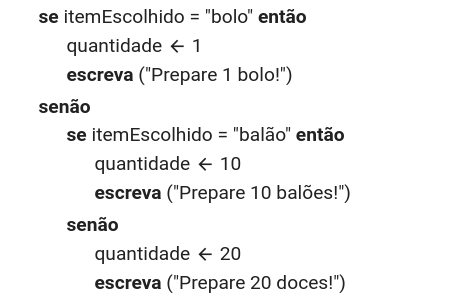
\includegraphics[scale=0.5]{figuras/atividade_festa_1.png}}
        \caption{Pseudocódigo referente à Pergunta 1}
        \label{figure:atividade_festa_1}
    \end{subfigure}
    \par\bigskip % force a bit of vertical whitespace
    \begin{subfigure}[t]{0.5\textwidth}
        \centering
        \setlength{\fboxrule}{0.1pt} % espessura da borda da figura
        \fbox{
\includegraphics[scale=0.5]{figuras/atividade_festa_2.png}}
        \caption{Pseudocódigo referente à Pergunta 2}
        \label{figure:atividade_festa_2}
    \end{subfigure}
    \par\bigskip % force a bit of vertical whitespace
    \begin{subfigure}[t]{0.5\textwidth}
        \centering
        \setlength{\fboxrule}{0.1pt} % espessura da borda da figura
        \fbox{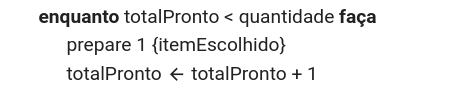
\includegraphics[scale=0.5]{figuras/atividade_festa_3.png}}
        \caption{Pseudocódigo referente à Pergunta 3}
        \label{figure:atividade_festa_3}
    \end{subfigure}
    \par\bigskip % force a bit of vertical whitespace
    \begin{subfigure}[t]{0.5\textwidth}
        \centering
        \setlength{\fboxrule}{0.1pt} % espessura da borda da figura
        \fbox{
\includegraphics[scale=0.5]{figuras/atividade_festa_4.png}}
        \caption{Pseudocódigo referente à Pergunta 4}
        \label{figure:atividade_festa_4}
    \end{subfigure}
    \par\bigskip % force a bit of vertical whitespace
    \begin{subfigure}[t]{0.5\textwidth}
        \centering
        \setlength{\fboxrule}{0.1pt} % espessura da borda da figura
        \fbox{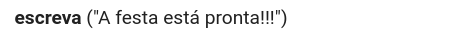
\includegraphics[scale=0.5]{figuras/atividade_festa_5.png}}
        \caption{Pseudocódigo referente à Pergunta 5}
        \label{figure:atividade_festa_5}
    \end{subfigure}
    \par\bigskip % force a bit of vertical whitespace
    \begin{subfigure}[t]{0.5\textwidth}
        \centering
        \setlength{\fboxrule}{0.1pt} % espessura da borda da figura
        \fbox{
\includegraphics[scale=0.5]{figuras/atividade_festa_6.png}}
        \caption{Pseudocódigo referente à Pergunta 6}
        \label{figure:atividade_festa_6}
    \end{subfigure}
    \caption{Trechos de pseudocódigo apresentados em cada pergunta da atividade de aprendizado referente à simulação \enquote{Planejando a Festa}.}
    \label{figure:atividade_festa}
\end{figure}

\begin{figure}[h!]
    \centering
    \setlength{\fboxrule}{0.1pt} % espessura da borda da figura
    \fbox{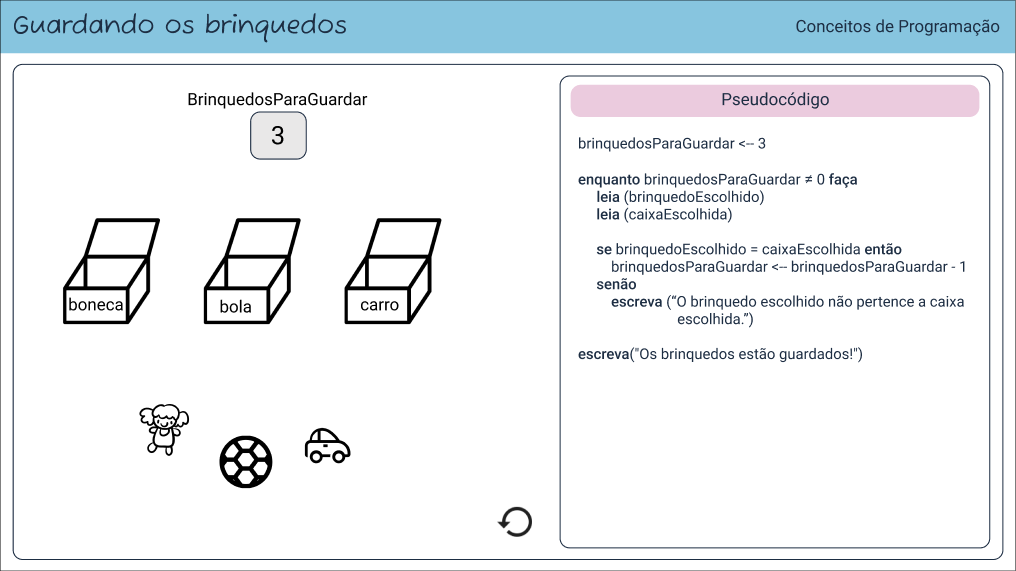
\includegraphics[scale=0.42]{prototipo_brinquedos_formulario.png}}
    \caption{Protótipo da simulação \enquote{Guardando os Brinquedos} apresentado na atividade de aprendizado para fornecer contexto para as questões.}
    \label{figure:brinquedos_forms}
\end{figure}

\begin{figure}[h!]
    \centering
    \begin{subfigure}[t]{0.5\textwidth}
        \centering
        \setlength{\fboxrule}{0.1pt} % espessura da borda da figura
        \fbox{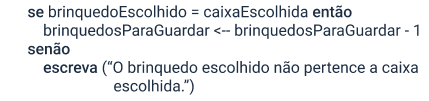
\includegraphics[scale=0.5]{figuras/atividade_brinquedos_1.png}}
        \caption{Pseudocódigo referente à Pergunta 1}
        \label{figure:atividade_brinquedos_1}
    \end{subfigure}
    \par\bigskip % force a bit of vertical whitespace
    \begin{subfigure}[t]{0.5\textwidth}
        \centering
        \setlength{\fboxrule}{0.1pt} % espessura da borda da figura
        \fbox{
\includegraphics[scale=0.5]{figuras/atividade_brinquedos_2.png}}
        \caption{Pseudocódigo referente à Pergunta 2}
        \label{figure:atividade_brinquedos_2}
    \end{subfigure}
    \par\bigskip % force a bit of vertical whitespace
    \begin{subfigure}[t]{0.5\textwidth}
        \centering
        \setlength{\fboxrule}{0.1pt} % espessura da borda da figura
        \fbox{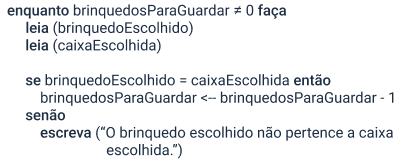
\includegraphics[scale=0.5]{figuras/atividade_brinquedos_3.png}}
        \caption{Pseudocódigo referente à Pergunta 3}
        \label{figure:atividade_brinquedos_3}
    \end{subfigure}
    \par\bigskip % force a bit of vertical whitespace
    \begin{subfigure}[t]{0.5\textwidth}
        \centering
        \setlength{\fboxrule}{0.1pt} % espessura da borda da figura
        \fbox{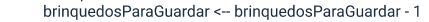
\includegraphics[scale=0.5]{figuras/atividade_brinquedos_4.png}}
        \caption{Pseudocódigo referente à Pergunta 4}
        \label{figure:atividade_brinquedos_4}
    \end{subfigure}
    \par\bigskip % force a bit of vertical whitespace
    \begin{subfigure}[t]{0.5\textwidth}
        \centering
        \setlength{\fboxrule}{0.1pt} % espessura da borda da figura
        \fbox{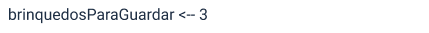
\includegraphics[scale=0.5]{figuras/atividade_brinquedos_5.png}}
        \caption{Pseudocódigo referente à Pergunta 5}
        \label{figure:atividade_brinquedos_5}
    \end{subfigure}
    \par\bigskip % force a bit of vertical whitespace
    \begin{subfigure}[t]{0.5\textwidth}
        \centering
        \setlength{\fboxrule}{0.1pt} % espessura da borda da figura
        \fbox{
\includegraphics[scale=0.5]{figuras/atividade_brinquedos_6.png}}
        \caption{Pseudocódigo referente à Pergunta 6}
        \label{figure:atividade_brinquedos_6}
    \end{subfigure}
    \caption{Trechos de pseudocódigo apresentados em cada pergunta da atividade de aprendizado referente à simulação \enquote{Guardando os Brinquedos}.}
    \label{figure:atividade_brinquedos}
\end{figure}

O Capítulo~\ref{cap_resultados} apresenta os resultados da avaliação do MVP feita a partir das respostas dos formulários.

%!TeX root=../tese.tex
%("dica" para o editor de texto: este arquivo é parte de um documento maior)
% para saber mais: https://tex.stackexchange.com/q/78101

\chapter{Resultados da avaliação da simulação}
\label{cap_resultados}

Os resultados da avaliação da simulação se encontram divididos em duas seções. A primeira se refere ao formulário de usabilidade, no qual obtivemos 26 respostas dos alunos presentes. A segunda é referente às respostas da atividade de aprendizado, na qual tivemos 13 respostas. Em virtude do tempo limitado durante a aula, alguns dos alunos não conseguiram terminar de preencher o segundo formulário, da atividade de aprendizado, por isso, obtivemos menos respostas nele.

\section{Formulário de usabilidade}

O formulário de usabilidade adaptado do questionário SUS foi preenchido pelos alunos logo após eles terminarem de explorar a simulação. Dos 26 alunos que o responderam, 12 não haviam tido contato anterior com programação e 14 já haviam tido. Para analisar as respostas, separamos os resultados entre esses dois grupos de estudantes.

A Figura \ref{figure:likert_sim} apresenta as respostas dos alunos que haviam tido contato anterior com programação. Dentro desse grupo de alunos, a maioria respondeu que gostaria de explorar mais a simulação (85,8\%). Apenas 14,3\% ficaram confusos com a ferramenta, sendo que 64,3\% dos estudantes concordaram que ela foi fácil de usar. Ademais, 64,3\% desses alunos acreditam que não precisariam de ajuda para explorar o MVP e 21,4\% precisariam. Em consonância, 64,3\% responderam que sabiam o que era preciso fazer para usar a simulação. Também podemos observar que somente 21,4\% das crianças acharam que algumas coisas na simulação não fizeram sentido e 14,3\% delas, que tiveram que fazer algumas coisas estranhas na ferramenta. Além disso, a maioria dos usuários (78,6\%) acredita que seus amigos poderiam aprender a usar a simulação muito rápido e se sentiram confiantes enquanto a exploravam. Por fim, 28,6\% dos alunos acham que tiveram que aprender muitas coisas antes de usar o MVP, enquanto a maioria discorda (57,2\%).

\begin{figure}[h!]
    \centering
    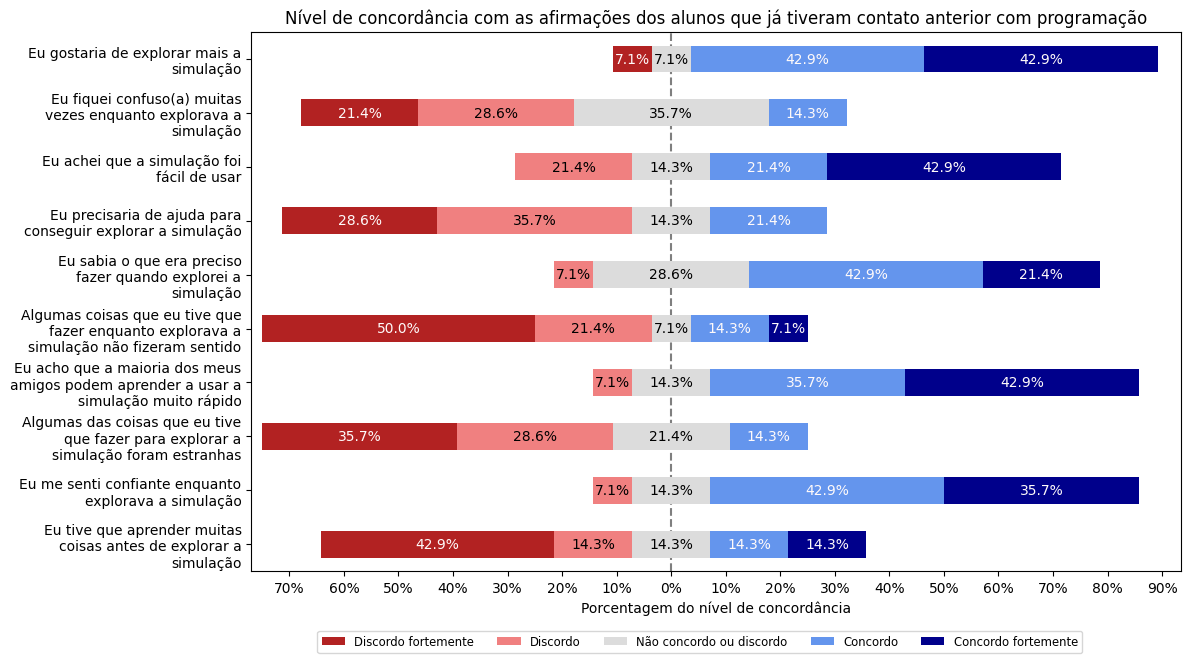
\includegraphics[scale=0.5]{likert_com_conhecimento.png}
    \caption{Porcentagem do nível de concordância com as afirmações dos alunos que já tiveram contato anterior com programação.}
    \label{figure:likert_sim}
\end{figure}

\begin{figure}[h!]
    \centering
    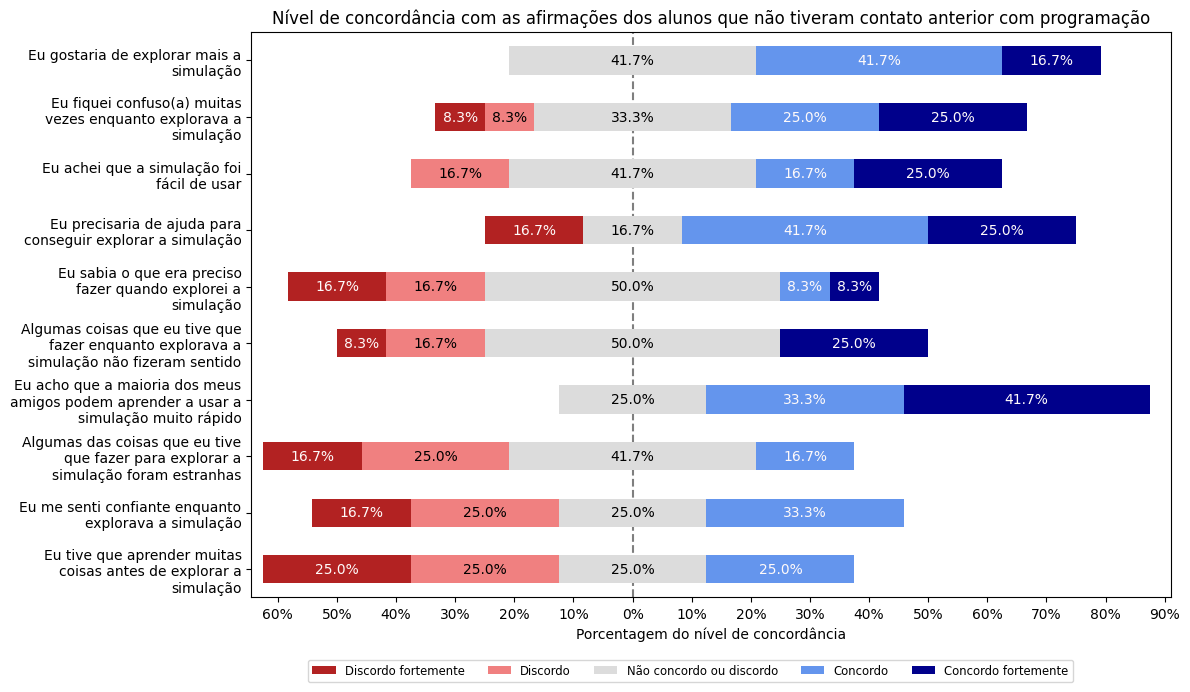
\includegraphics[scale=0.5]{likert_sem_conhecimento.png}
    \caption{Porcentagem do nível de concordância com as afirmações dos alunos que não tiveram contato anterior com programação.}
    \label{figure:likert_nao}
\end{figure}


Já na Figura \ref{figure:likert_nao}, podemos observar as respostas dos alunos que não tiveram contato anterior com programação. Dentre eles, mais da metade (58,4\%) respondeu que gostaria de explorar mais a simulação, porém um grande número (41,7\%) não concordou nem discordou da afirmação. Ainda, 50\% dos alunos desse grupo relatou que ficou confuso muitas vezes enquanto explorava o MVP e 33,3\% não concordou nem discordou disso. A maioria (66,7\%) também achou que precisaria de ajuda para usar a simulação e apenas 16,6\% sabia o que era preciso fazer quando usou a ferramenta. Neste último caso, 50\% não concordou nem discordou da afirmação. De forma contraditória, 41,7\% acharam que a ferramenta foi fácil de usar e apenas 16,7\% discordaram. Ademais, metade dos alunos não concordaram nem discordaram de que algumas coisas que tiveram que fazer não fizeram sentido, e apenas 16,7\% acharam que algumas coisas foram estranhas, enquanto 41,7\% não concordaram nem discordaram. Apesar das respostas anteriores, a maioria dos usuários (72\%) acredita que seus amigos poderiam aprender a usar a simulação muito rápido e apenas 25\% acha que teve que aprender muitas coisas antes de explorá-la. Por fim, 33,3\% das crianças relataram que se sentiram confiantes ao explorar o MVP enquanto 41,7\% discordaram.


Ademais, a Figura \ref{figure:radar_medias} apresenta a média dos níveis de concordância com cada afirmativa dos dois grupos de alunos.

\begin{figure}[h!]
    \centering
    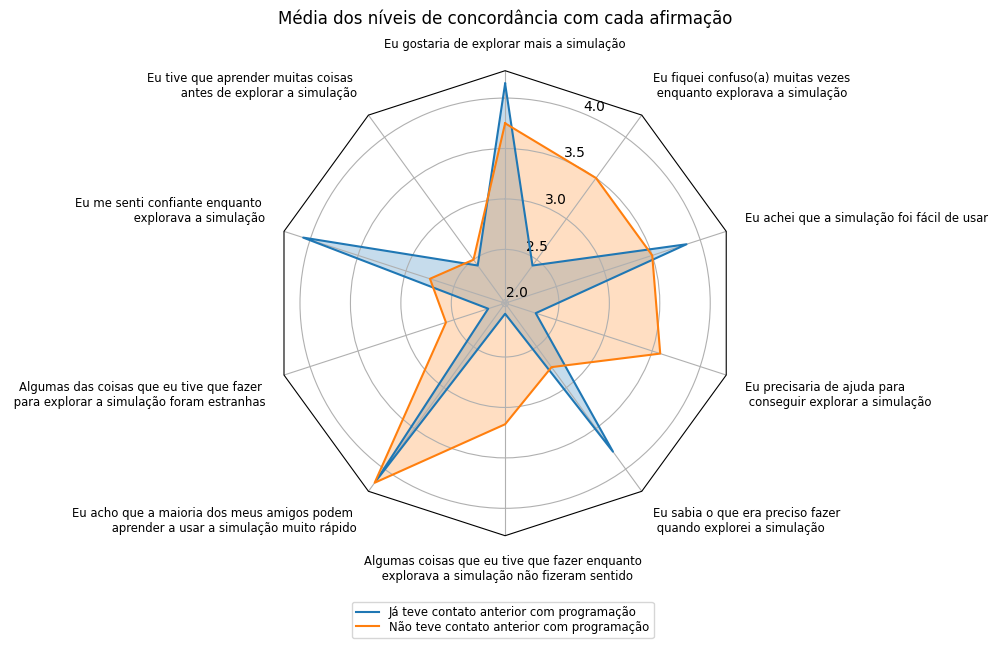
\includegraphics[scale=0.62]{radar_medias.png}
    \caption{Média dos níveis de concordância com cada afirmação dos alunos que já tiveram contato anterior com programação e dos que não tiveram. Cada raio do gráfico representa a média para uma afirmação do formulário.}
    \label{figure:radar_medias}
\end{figure}

Podemos observar que as afirmações do formulário SUS apresentam duas conotações contrárias, tendo algumas delas um sentimento positivo em relação a ferramenta avaliada e outras um sentimento negativo. No questionário, as questões estão intercaladas, de forma que a primeira apresenta um sentimento positivo, a segunda apresenta um sentimento negativo, e assim por diante. Assim, analisando as respostas dos alunos que já tinham um contato prévio com programação, podemos notar que elas estão dentro do esperado, ou seja, em média, os estudantes concordam com as afirmações de caráter positivo e discordam daquelas de caráter negativo. Isso indica que o MPV projetado demonstrou potencial para a continuação ou complementação do aprendizado dos conceitos de lógica de programação das crianças.

Em relação às respostas dos alunos que não tinham contato prévio com programação, observamos algumas inconsistências entre os níveis de concordância com as afirmações de caráter positivo e negativo. Encontramos muitas respostas concordando com afirmações complementares de conotações contrárias. Além disso, em pelo menos metade das afirmações, grande parte dos estudantes permaneceu neutro, optando por não concordar ou discordar, o que não aconteceu com o grupo anterior. Porém, apesar de obtermos muitas respostas concordantes com as afirmações com sentimento negativo em relação ao MVP, a maioria dos estudantes concordou que gostaria de explorar mais a simulação e que seus amigos poderiam aprender a usá-la muito rápido, mostrando o potencial da ferramenta. A partir dessas respostas, verificamos a necessidade de melhorar a forma de introduzir os conceitos de lógica de programação para aqueles que nunca tiveram contato com Computação.

Ademais, calculamos as pontuações SUS, na escala de 0 a 100, para as respostas dos dois grupos de alunos. Para os alunos que já tiveram contato anterior com programação, obtivemos uma média de \textit{score} de 71,6, indicando uma boa usabilidade para o MVP, segundo \citet{bangor2009determining}. Para aqueles que não tinham contato anterior com Computação, a média de pontuação calculada foi de 53,9, o que demonstra usabilidade razoável para a ferramenta de acordo com os autores.

\begin{table}[h!]
\centering
\begin{tabular}{c|c|c|}
\cline{2-3}
                                     & \textbf{\begin{tabular}[c]{@{}c@{}}Já tiveram contato\\ anterior com programação\end{tabular}} & \textbf{\begin{tabular}[c]{@{}c@{}}Não tiveram contato\\ anterior com programação\end{tabular}} \\ \cline{2-3} 
                                     & 82,5                                                                                           & 55                                                                                              \\ \cline{2-3} 
                                     & 75                                                                                             & 50                                                                                              \\ \cline{2-3} 
                                     & 100                                                                                            & 47,5                                                                                            \\ \cline{2-3} 
                                     & 65                                                                                             & 47,5                                                                                            \\ \cline{2-3} 
                                     & 75                                                                                             & 65                                                                                              \\ \cline{2-3} 
                                     & 77,5                                                                                           & 30                                                                                              \\ \cline{2-3} 
                                     & 65                                                                                             & 87,5                                                                                            \\ \cline{2-3} 
                                     & 67,5                                                                                           & 50                                                                                              \\ \cline{2-3} 
                                     & 60                                                                                             & 57,5                                                                                            \\ \cline{2-3} 
                                     & 62,5                                                                                           & 40                                                                                              \\ \cline{2-3} 
                                     & 72,5                                                                                           & 50                                                                                              \\ \cline{2-3} 
                                     & 37,5                                                                                           & 67,5                                                                                            \\ \cline{2-3} 
                                     & 97,5                                                                                           & -                                                                                               \\ \cline{2-3} 
                                     & 65                                                                                             & -                                                                                               \\ \hline
\multicolumn{1}{|c|}{\textbf{média}} & 71,6                                                                                           & 53,9                                                                                            \\ \hline
\end{tabular}
\caption{Pontuação SUS calculada para cada aluno, com as médias para alunos que já tiveram contato anterior com programação e para os que não tiveram.}
\label{table:sus_score}
\end{table}

\subsection**{Opiniões e sugestões sobre a simulação}

Em relação as questões dissertativas sobre opiniões e sugestões da simulação, apresentadas ao final do formulário de usabilidade, quando questionado o que mais gostaram na ferramenta, no geral, as crianças relataram que gostaram da experiência. Dividimos as respostas em quatro categorias baseadas nos temas que se destacaram no \textit{feedback}: recursos específicos, interatividade, experiência de aprendizado e experiência geral. A Figura \ref{figure:livre_1} apresenta os relatos dos estudantes divididos nessas categorias.

\begin{figure}[h!]
    \centering
    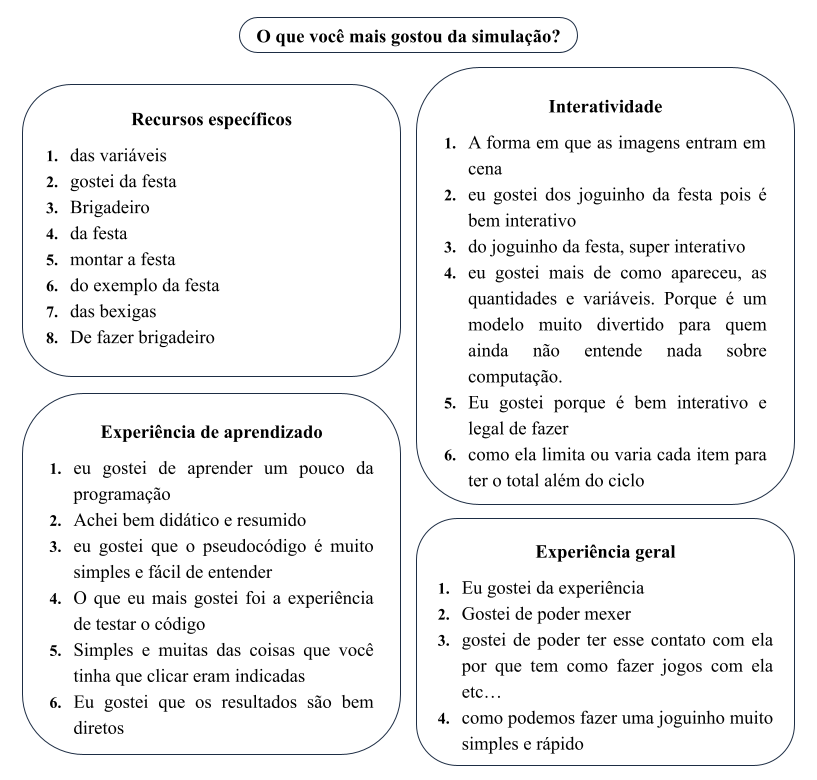
\includegraphics[scale=0.5]{formulario_livre_1.png}
    \caption{Respostas dos alunos em relação à pergunta livre \enquote{O que você mais gostou da simulação?}, divididas em categorias.}
    \label{figure:livre_1}
\end{figure}

Assim, dentre o que as crianças mais gostaram, muitos relataram recursos específicos, como preparar um determinado item para a festa. Além disso, algumas respostas ressaltaram a interatividade da simulação como ponto positivo, como os elementos visuais se apresentavam. Outros relatos destacaram boas experiências de aprendizado e no geral, descrevendo o MVP como didático, simples e direto.

Sobre o que menos gostaram da simulação, observamos outras quatro categorias em que se encaixavam os temas de respostas dos alunos: experiência positiva geral, confusão ou dificuldade, \textit{design} ou problemas de interação, e conteúdo ou tarefas. A Figura \ref{figure:livre_2} apresenta os relatos dos estudantes divididos nessas categorias. Muitos alunos não observaram pontos negativos na experiência geral com a simulação. Por outro lado, muitos encontraram dificuldades e relataram que ficaram confusos, principalmente com o pseudocódigo, ou que acharam complicado. Algumas crianças também apontaram alguns problemas de \textit{design} ou interatividade no MVP e limitações nas possíveis tarefas.

\begin{figure}[h!]
    \centering
    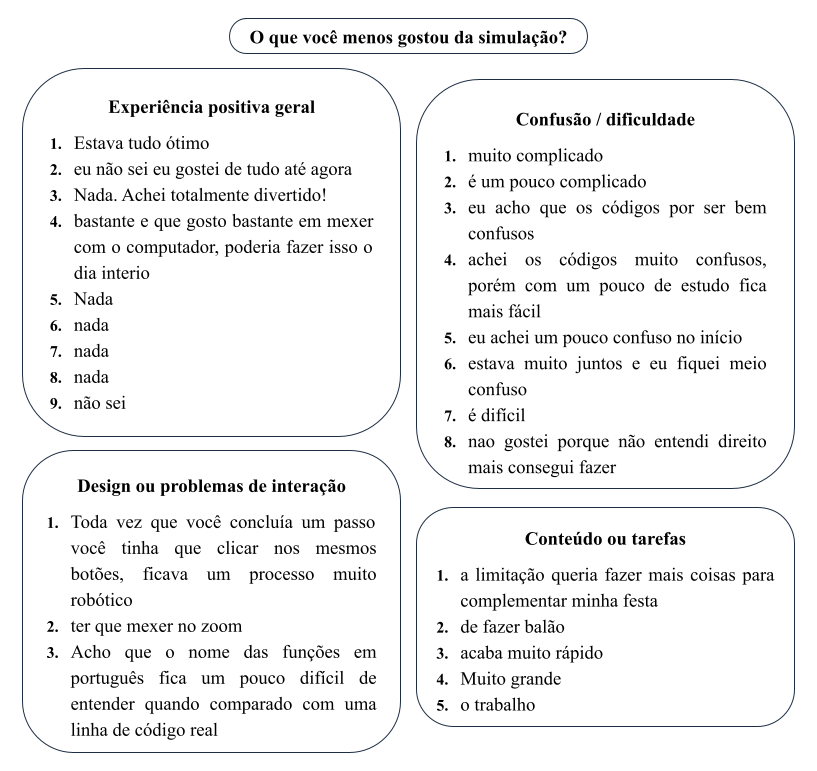
\includegraphics[scale=0.5]{formulario_livre_2.png}
    \caption{Respostas dos alunos em relação à pergunta livre \enquote{O que você menos gostou da simulação?}, divididas em categorias.}
    \label{figure:livre_2}
\end{figure}

Por fim, recebemos comentários referentes a apreciação e divertimento em relação à experiência com a simulação, e complexidade dela, além de sugestões para organizar os códigos, como mostra a Figura \ref{figure:livre_3}. A partir das opiniões e sugestões recebidas nas três questões livres, podemos também constatar a necessidade de algumas modificações nas interações da simulação, bem como na apresentação do pseudocódigo correspondente para tentar diminuir a complexidade encontrada por alguns e melhorar a usabilidade da ferramenta.

\begin{figure}[h!]
    \centering
    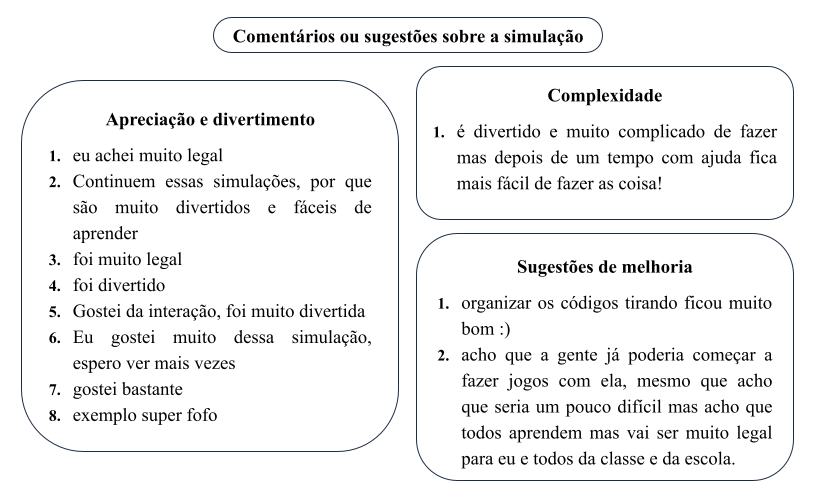
\includegraphics[scale=0.5]{formulario_livre_3.png}
    \caption{Respostas dos alunos em relação à pergunta livre sobre comentários e sugestões da simulação, divididas em categorias.}
    \label{figure:livre_3}
\end{figure}

\section{Atividade de aprendizado}

O questionário com a atividades de aprendizado foi respondido por 13 alunos após o preenchimento do formulário anterior. Das 13 respostas, 6 foram de alunos que nunca tiveram contanto com programação e 7 de alunos que já tiveram. Ainda, dos 6 alunos, apenas 3 responderam a segunda parte da atividade, referente à simulação \enquote{Guardando os Brinquedos}. Para analisar as respostas, separamos os resultados entre os dois grupos de estudantes.

\subsection{Perguntas sobre a simulação \enquote{Planejando a Festa}}

A Figura \ref{figure:pies_festa} apresenta as respostas dos alunos às questões relacionadas à simulação \enquote{Planejando a Festa}. A pergunta 1 tinha como resposta o conceito de \enquote*{condicional}. Considerando os alunos que já tinham um contato anterior com programação, 42,9\% acertou esta questão, outros 42,9\% escolheram o conceito de \enquote*{variáveis} e 14,3\%, o de \enquote*{saída}. Dentre os demais alunos, que nunca tiveram contato com Computação, 33,3\% escolheu a resposta certa, enquanto 50\% respondeu \enquote*{variáveis} e 14,3\% escolheu \enquote*{saída}. Podemos observar que houve confusão entre o conceito de \enquote*{condicional} e o de \enquote*{variáveis} e \enquote*{saída} pelos dois grupos de estudantes. Entretanto, no trecho de pseudocódigo apresentado nessa questão (Figura \ref{figure:atividade_festa_1}) temos a repetição dos dois conceitos que foram confundidos como resposta na execução dentro dos condicionais, o que poderia explicar o engano.

No caso da questão 2, que tinha como resposta \enquote*{variáveis}, observamos que houve uma confusão entre esse conceito e o de \enquote*{entrada}, que também foi notada no geral. Nessa pergunta, 57,1\% dos alunos com conhecimento prévio de Computação acertaram a resposta enquanto 42,9\% escolheram \enquote*{entrada}. Dos alunos que não tinham conhecimento prévio, tivemos um número menor de acertos (33,3\%) e o restante também respondeu \enquote*{entrada}.

\begin{figure}[h!]
    \centering
    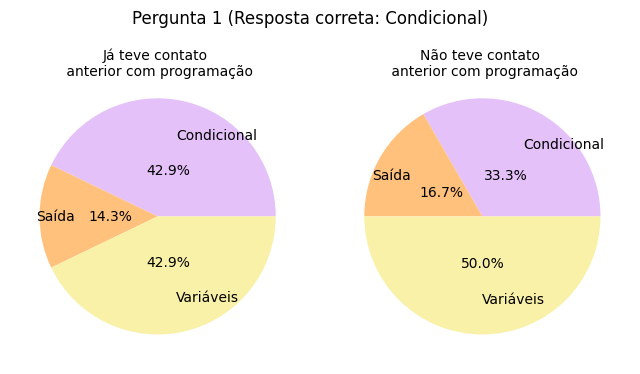
\includegraphics[scale=0.46]{pie_festa_p1.png}
    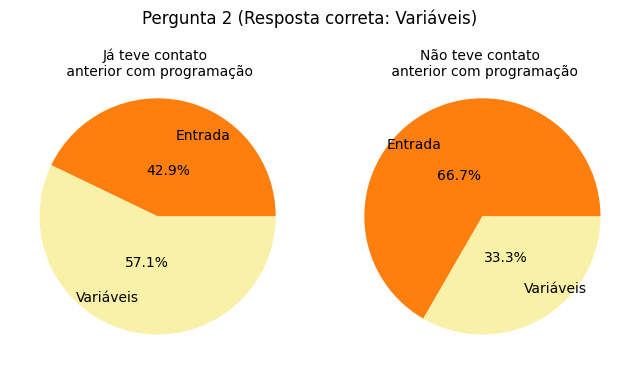
\includegraphics[scale=0.46]{pie_festa_p2.png}
    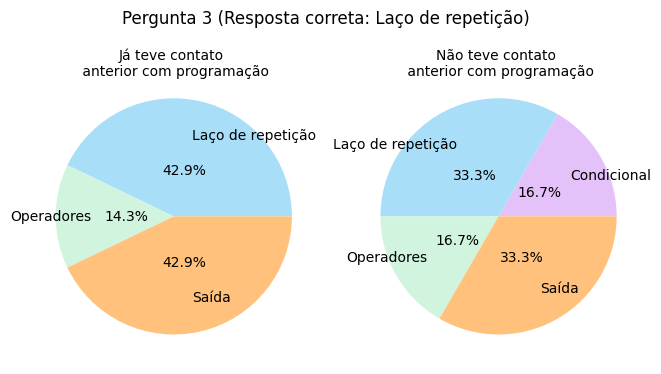
\includegraphics[scale=0.46]{pie_festa_p3.png}
    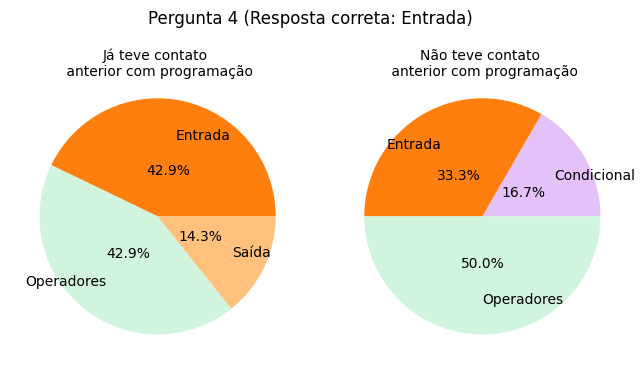
\includegraphics[scale=0.45]{pie_festa_p4.png}
    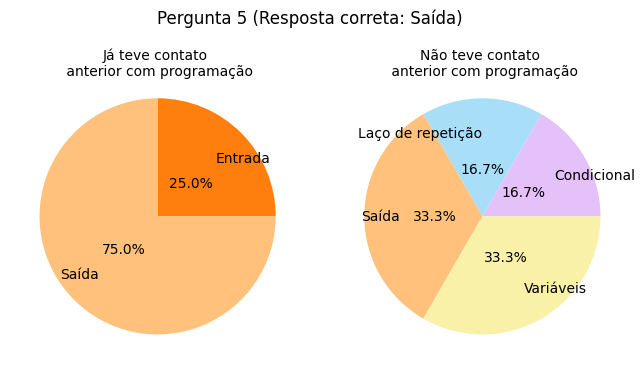
\includegraphics[scale=0.45]{pie_festa_p5.png}
    \includegraphics[scale=0.44]{pie_festa_p6.png}
    \includegraphics[scale=0.35]{pie_legend.png}
    \caption{Porcentagens das respostas dos alunos às perguntas da atividade de aprendizado relacionada à simulação \enquote{Planejando a Festa}. Para cada pergunta, apresentamos as respostas dos alunos que já tiveram contanto anterior com Computação à esquerda e as dos que não tiveram à direita.}
    \label{figure:pies_festa}
\end{figure}

Já na pergunta 3, a resposta correta era \enquote*{laço de repetição}. Das crianças que tiveram contato anterior com programação, 42,9\% acertaram a questão e os demais responderam \enquote*{saída} (42,9\%) e \enquote*{operadores} (14,3\%). Já entre os alunos que não tiveram contato anterior com Computação, 33,3\% escolheram a resposta correta, enquanto 33,3\% escolheram o conceito de \enquote*{saída}, 16,7\% de \enquote*{operadores} e outros 16,7\% de \enquote*{condicional}. Nesta questão tivemos muitas respostas divergentes, assim como na pergunta 1. O trecho de pseudocódigo apresentado nela (Figura \ref{figure:atividade_festa_3}) trazia além do laço de repetição, o conceito de operadores representado na condição do laço e dentro da execução dele, o que poderia justificar a escolha desta resposta por alguns alunos. Além disso, acreditamos também que a ação de preparar um item, a qual ocorre dentro do laço, possa ter sido confundida com o conceito de \enquote*{saída}, respondido por outros. Entretanto, a escolha do conceito de \enquote*{condicional} por alguns estudantes indica a falta de compreensão deles.

Nas três última questões, também observamos que não houve entendimento da maior parte dos alunos em relação aos conceitos de lógica de programação. A quarta pergunta do questionário tinha como resposta o conceito de \enquote*{entrada}. Nela, observamos que 42,9\% dos alunos com conhecimento em programação acertaram a questão. Outras resposta foram \enquote*{operadores} (42,9\%) e \enquote*{saída} (14,3\%). Dos alunos sem conhecimento prévio em Computação, 33,3\% escolheram a resposta certa, enquanto 50\% responderam \enquote*{operadores} e 16,7\% \enquote*{condicional}. 

Na pergunta 5, que tinha como resposta o conceito de \enquote*{saída}, a maioria das crianças com conhecimento anterior de programação acertou (75\%) e apenas 25\% confundiram com de \enquote*{entrada}. Dos alunos sem conhecimento anterior 33,3\% responderam corretamente e os demais alunos responderam \enquote*{variáveis} (33,3\%), \enquote*{condicional} (16,7\%) e \enquote*{laço de repetição} (16,7\%).

Por fim, na questão 6 a resposta correta era \enquote*{operadores} e poucos alunos acertaram o conceito apresentado. Entre as crianças que já tiveram contato com Computação, apenas 28,6\% acertou a resposta. A maior parte das respostas foi \enquote*{laço de repetição} (57,1\%) e os demais responderam \enquote*{condicional} (14,3\%). Entre os estudantes que nunca tiveram contato com programação, as respostas foram igualmente escolhidas entre \enquote*{operadores}, \enquote*{laço de repetição} e \enquote*{condicional}.

\subsection{Perguntas sobre a simulação \enquote{Guardando os Brinquedos}}

A Figura \ref{figure:pies_brinquedos} apresenta as respostas dos alunos às questões relacionadas à simulação \enquote{Guardando os Brinquedos}, com a qual não houve interação. As crianças apenas visualizaram a imagem de um estado da simulação e do pseudocódigo completo. No geral, podemos observar que as crianças com conhecimento prévio em programação fizeram mais confusões em relação aos conceitos de programação abordados do que os demais alunos.

A primeira pergunta tinha como resposta \enquote*{condicional} e, dos alunos que já tiveram contato com Computação, 85,7\% acertaram, enquanto 14,3\% responderam \enquote*{variáveis}. Entre aqueles que não conheciam programação, 66,7\% escolheram a resposta correta e 33,3\% responderam o conceito de \enquote*{saída}. Nesta questão, novamente, observamos que o trecho de pseudocódigo apresentado (Figura \ref{figure:atividade_brinquedos_1}) continha também os demais conceitos escolhidos como resposta por alguns estudantes, o que poderia explicar a confusão.

\begin{figure}[h!]
    \centering
    \includegraphics[scale=0.45]{pie_brinquedos_p1.png}
    \includegraphics[scale=0.45]{pie_brinquedos_p2.png}
    \includegraphics[scale=0.43]{pie_brinquedos_p3.png}
    \includegraphics[scale=0.44]{pie_brinquedos_p4.png}
    \includegraphics[scale=0.45]{pie_brinquedos_p5.png}
    \includegraphics[scale=0.44]{pie_brinquedos_p6.png}
    \includegraphics[scale=0.35]{pie_legend.png}
    \caption{Porcentagens das respostas dos alunos às perguntas da atividade de aprendizado relacionada à simulação \enquote{Guardando os Brinquedos}. Para cada pergunta, apresentamos as respostas dos alunos que já tiveram contanto anterior com Computação à esquerda e as dos que não tiveram à direita.}
    \label{figure:pies_brinquedos}
\end{figure}

Já na questão 2, cuja resposta era \enquote*{saída}, houve problemas de compreensão dos conceitos por parte da maioria das crianças. Entre aquelas que já conheciam programação, apenas 28,6\% acertaram a resposta, enquanto 42,9\% escolheram \enquote*{operadores} e 28,6\% escolheram \enquote*{entrada}. Entre os alunos que não conheciam Computação, 33,3\% deles acertaram e 66,7\% escolheram \enquote*{entrada}.

Na pergunta 3, em que a resposta correta era \enquote*{laço de repetição}, as duas crianças que não tinham contato anterior com Computação e responderam a questão, acertaram. Dentre os demais alunos, que já tiveram contato, 28,6\% acertaram a resposta e o restante escolheu os conceitos de \enquote*{saída} (28,6\%), \enquote*{condicional} (28,6\%) e \enquote*{entrada} (14,3\%). Porém, ressaltamos que todos os conceitos citados estavam presentes no trecho de pseudocódigo apresentado para eles na pergunta (Figura \ref{figure:atividade_brinquedos_3}).

Já a pergunta 4 tinha como resposta o conceito de \enquote*{operadores}. Entre os alunos que conheciam Computação, apenas 14,3\% acertaram a questão, e a maioria (42,9\%) respondeu \enquote*{variáveis}. Outros escolheram \enquote*{laço de repetição} (28,6\%) e \enquote*{condicional} (14,3\%). Entre os alunos que não tinham conhecimento, a maioria (66,7\%) acertou a resposta e 33,3\% respondeu \enquote*{laço de repetição}. Nessa questão, o trecho de pseudocódigo apresentado (Figura \ref{figure:atividade_brinquedos_4}) trazia uma operação sendo atribuída a uma variável. Assim, a confusão com o conceito de \enquote*{variáveis} pode ter ocorrido por isso. Entretanto, a escolha das demais respostas mostrou, novamente, a falta de compreensão dos conceitos de programação por parte das crianças.

Ademais, nas duas últimas questões, também observamos que não houve entendimento dos alunos em relação aos conceitos. Na questão 5, em que a resposta era \enquote*{variáveis}, dos alunos que tiveram contato anterior com programação, apenas 14,3\% acertaram, enquanto 42,9\% responderam \enquote*{entrada} e 42,9\% responderam \enquote*{condicional}. Dos estudantes sem conhecimento prévio, 66,7\% respondeu \enquote*{variáveis} e 33,3\% \enquote*{entrada}.

Finalmente, na pergunta 6, a resposta correta era \enquote*{entrada}. Entre as crianças que conheciam Computação, apenas 14,3\% acertou a resposta, 57,1\% apontaram de forma errada o conceito de \enquote*{laço de repetição} e 28,6\% o de \enquote*{saída}. Dentre os três alunos que nunca tiveram contato com programação, nenhum acertou essa questão, 66,7\% deles confundiu o conceito com o de \enquote*{variáveis} e 33,3\% escolheu \enquote*{saída}.

A partir desses resultados, observamos que o uso das simulações não cumpriu a finalidade de ensinar os conceitos de lógica de programação para as crianças. Entretanto, como observado, algumas confusões dos conceitos de programação pelos alunos podem ter sido causadas pela formulação das questões da atividade de aprendizado. A presença de muitos conceitos, que inclusive se repetiam, nos trechos de pseudocódigo apresentados em algumas questões pode ter gerado ambiguidade nas respostas. Ainda assim, aqueles conceitos que foram apresentados de forma isolada, como o trecho de \enquote*{variáveis}, não poderia ter sido confundido com o de \enquote*{condicional}, por exemplo, sendo completamente desrelacionado. Isso também indica a falta  de entendimento do conteúdo apresentado.

Ademais, notamos que os alunos sem conhecimento prévio em programação tiveram um maior número de acertos nas questões relacionadas à simulação \enquote{Guardando os Brinquedos}, com a qual eles não interagiram. Isso poderia sugerir a necessidade de alterações e melhorias nas interações implementadas na simulação \enquote{Planejando a Festa}. Por fim, acreditamos que, no geral, os resultados indicaram a necessidade de diversas reformulações para o MVP, implicando em uma nova iteração nos ciclos de \textit{design} e engenharia de DSR.


%!TeX root=../main.tex
%("dica" para o editor de texto: este arquivo é parte de um documento maior)
% para saber mais: https://tex.stackexchange.com/q/78101

\chapter{Considerações Finais}

\section{Limitações e Trabalhos Futuros}

\section{Conclusões}


%%%%%%%%%%%%%%%%%%%%%%%%%%%% APÊNDICES E ANEXOS %%%%%%%%%%%%%%%%%%%%%%%%%%%%%%%%

% Um apêndice é algum conteúdo adicional de sua autoria que faz parte e
% colabora com a ideia geral do texto mas que, por alguma razão, não precisa
% fazer parte da sequência do discurso; por exemplo, a demonstração de um
% teorema intermediário, as perguntas usadas em uma pesquisa qualitativa etc.
%
% Um anexo é um documento que não faz parte da tese (em geral, nem é de sua
% autoria) mas é relevante para o conteúdo; por exemplo, a especificação do
% padrão técnico ou a legislação que o trabalho discute, um artigo de jornal
% apresentando a percepção do público sobre o tema da tese etc.
%
% Os comandos appendix e annex reiniciam a numeração de capítulos e passam
% a numerá-los com letras. "annex" não faz parte de nenhuma classe padrão,
% foi criado para este modelo. Se o trabalho não tiver apêndices ou anexos,
% remova estas linhas.
%
% Diferentemente de \mainmatter, \backmatter etc., \appendix e \annex não
% forçam o início de uma nova página. Em geral isso não é importante, pois
% o comando seguinte costuma ser "\chapter", mas pode causar problemas com
% a formatação dos cabeçalhos. Assim, vamos forçar uma nova página antes
% de cada um deles.

%%%% Apêndices %%%%

% \cleardoublepage

% \pagestyle{appendix}

% \appendix

% % \addappheadtotoc acrescenta a palavra "Apêndice" ao sumário; se
% % só há apêndices, sem anexos, provavelmente não é necessário.
% \addappheadtotoc

% \input{conteudo/apendice-exemplo-faq}
% \par

% %%%% Anexos %%%%

% \cleardoublepage

% \pagestyle{appendix} % repete o anterior, caso você não use apêndices

% \annex

% % \addappheadtotoc acrescenta a palavra "Anexo" ao sumário; se
% % só há anexos, sem apêndices, provavelmente não é necessário.
% \addappheadtotoc

% \input{conteudo/anexo-exemplo-imegoodies}
% \par
% \input{conteudo/anexo-exemplo-pseudocodigo}
% \par


%%%%%%%%%%%%%%% SEÇÕES FINAIS (BIBLIOGRAFIA E ÍNDICE REMISSIVO) %%%%%%%%%%%%%%%%

% O comando backmatter desabilita a numeração de capítulos.
\backmatter

\pagestyle{backmatter}

% Espaço adicional no sumário antes das referências / índice remissivo
\addtocontents{toc}{\vspace{2\baselineskip plus .5\baselineskip minus .5\baselineskip}}

% A bibliografia é obrigatória

\printbibliography[
  title=\refname\label{sec:bib}, % "Referências", recomendado pela ABNT
  %title=\bibname\label{sec:bib}, % "Bibliografia"
  heading=bibintoc, % Inclui a bibliografia no sumário
]

% \printindex % imprime o índice remissivo no documento (opcional)

\end{document}
